%\PassOptionsToPackage{draft}{graphicx}
\documentclass[10pt,aspectratio=169,dvipsnames]{beamer} % aspect ratio 16:9
%\graphicspath{{../../figures/}}

%\includeonlyframes{frame1,frame2,frame3}

%%%%%%%%%%%%%%%%%%%%%%%%%%%%%%%%%%%%%%%%%%%%%%%%%%
% Packages
%%%%%%%%%%%%%%%%%%%%%%%%%%%%%%%%%%%%%%%%%%%%%%%%%%
\usepackage{appendixnumberbeamer}
\usepackage{booktabs}
\usepackage{csvsimple} % for csv read
%\usepackage[scale=2]{ccicons}
\usepackage{pgfplots}
\usepackage{xspace}
%\usepackage{amsmath}
\usepackage{totcount}
\usepackage{tikz}
\usepackage{bm}
\usepackage{float}
\usepackage{eso-pic} 
\usepackage{wrapfig}
\usepackage{animate,media9}
\usepackage{subfig}
\usepackage{fancybox}
%\usepackage{multimedia}
\usepackage{dashbox}
\usepackage{tcolorbox}
\usepackage{multicol}
\usepackage{multirow}
\usepackage{xcolor}
\usepackage[document]{ragged2e}
\usepackage{caption}
\usepackage{comment}
\usepackage{mathtools}% Loads amsmath
\usepackage{movie15}

%\usepackage[export]{adjustbox}
%\usepackage{background}
%\backgroundsetup{contents=preliminary,placement=bottom,color=blue}
%\usepackage{FiraSans}

%\usepackage{comment}
%\usetikzlibrary{external} % speedup compilation
%\tikzexternalize % activate!
%\usetikzlibrary{shapes,arrows} 

%\usepackage{bibentry}
%\nobibliography*
\usepackage{ifthen}
\newcounter{angle}
\setcounter{angle}{0}
%\usepackage{bibentry}
%\nobibliography*
\usepackage{caption}%

\graphicspath{{figures/}}

\captionsetup[figure]{labelformat=empty}%
\usefonttheme{structurebold}
%%%%%%%%%%%%%%%%%%%%%%%%%%%%%%%%%%%%%%%%%%%%%%%%%%
% Metropolis theme custom modification file
%%%%%%%%%%%%%%%%%%%%%%%%%%%%%%%%%%%%%%%%%%%%%%%%%%
% Metropolis theme custom modification file
%%%%%%%%%%%%%%%%%%%%%%%%%%%%%%%%%%%%%%%%%%%%%%%%%%
% Metropolis theme custom colors
%%%%%%%%%%%%%%%%%%%%%%%%%%%%%%%%%%%%%%%%%%%%%%%%%%
\usetheme[progressbar=foot]{metropolis}
\useoutertheme{metropolis}
\useinnertheme{metropolis}
\usefonttheme{metropolis}
\setbeamercolor{background canvas}{bg=white}

%\usecolortheme{spruce}

\definecolor{myblue}{rgb}{0.19,0.55,0.91}
\definecolor{mediumblue}{rgb}{0,0,205}
\definecolor{darkblue}{rgb}{0,0,139}
\definecolor{Dodgerblue}{HTML}{1E90FF}
\definecolor{Navy}{HTML}{000080} % {rgb}{0,0,128}
\definecolor{Aliceblue}{HTML}{F0F8FF}
\definecolor{Lightskyblue}{HTML}{87CEFA}
\definecolor{logoblue}{RGB}{1,67,140}
\definecolor{Purple}{HTML}{911146}
\definecolor{Orange}{HTML}{CF4A30}

\setbeamercolor{progress bar}{bg=Lightskyblue}
\setbeamercolor{progress bar}{ fg=logoblue} 
\setbeamercolor{frametitle}{bg=logoblue}
\setbeamercolor{title separator}{fg=logoblue}
\setbeamercolor{block title}{bg=Lightskyblue!30,fg=black}
\setbeamercolor{block body}{bg=Lightskyblue!15,fg=black}
\setbeamercolor{alerted text}{fg=Purple}
% notes colors
\setbeamercolor{note page}{bg=white}
\setbeamercolor{note title}{bg=Lightskyblue}
%%%%%%%%%%%%%%%%%%%%%%%%%%%%%%%%%%%%%%%%%%%%%%%%%%
%  Theme modifications
%%%%%%%%%%%%%%%%%%%%%%%%%%%%%%%%%%%%%%%%%%%%%%%%%%
% modify progress bar linewidth
\makeatletter
\setlength{\metropolis@progressinheadfoot@linewidth}{2pt} 
\setlength{\metropolis@titleseparator@linewidth}{1pt}
\setlength{\metropolis@progressonsectionpage@linewidth}{1pt}

\setbeamertemplate{progress bar in section page}{
	\setlength{\metropolis@progressonsectionpage}{%
		\textwidth * \ratio{\thesection pt}{\totvalue{totalsection} pt}%
	}%
	\begin{tikzpicture}
		\fill[bg] (0,0) rectangle (\textwidth, 
		\metropolis@progressonsectionpage@linewidth);
		\fill[fg] (0,0) rectangle (\metropolis@progressonsectionpage, 
		\metropolis@progressonsectionpage@linewidth);
	\end{tikzpicture}%
}
\makeatother
\newcounter{totalsection}
\regtotcounter{totalsection}

\AtBeginDocument{%
	\pretocmd{\section}{\refstepcounter{totalsection}}{\typeout{Yes, prepending 
	was successful}}{\typeout{No, prepending was not successful}}%
}%
%%%%%%%%%%%%%%%%%%%%%%%%%%%%%%%%%%%%%%%%%%%%%%%%%%
%  Bibliography mods
%%%%%%%%%%%%%%%%%%%%%%%%%%%%%%%%%%%%%%%%%%%%%%%%%%
\setbeamertemplate{bibliography item}{\insertbiblabel} %% Remove book symbol 
%%from references and add number in square brackets
% kill the abominable icon (without number)
%\setbeamertemplate{bibliography item}{}
%\makeatletter
%\renewcommand\@biblabel[1]{#1.} % number only
%\makeatother
% remove line breaks in bibliography
\setbeamertemplate{bibliography entry title}{}
\setbeamertemplate{bibliography entry location}{}
%%%%%%%%%%%%%%%%%%%%%%%%%%%%%%%%%%%%%%%%%%%%%%%%%%
%  Bibliography custom commands
%%%%%%%%%%%%%%%%%%%%%%%%%%%%%%%%%%%%%%%%%%%%%%%%%%
\newcommand{\bibliotitlestyle}[1]{\textbf{#1}\par}

\newif\ifinbiblio
\newcounter{bibkey}
\newenvironment{biblio}[2][long]{%
	%\setbeamertemplate{bibliography item}{\insertbiblabel}
	\setbeamertemplate{bibliography item}{}% without numbers
	\setbeamerfont{bibliography item}{size=\footnotesize}
	\setbeamerfont{bibliography entry author}{size=\footnotesize}
	\setbeamerfont{bibliography entry title}{size=\footnotesize}
	\setbeamerfont{bibliography entry location}{size=\footnotesize}
	\setbeamerfont{bibliography entry note}{size=\footnotesize}
	\ifx!#2!\else%
	\bibliotitlestyle{#2}%
	\fi%
	\begin{thebibliography}{}%
		\inbibliotrue%
		\setbeamertemplate{bibliography entry title}[#1]%
	}{%
		\inbibliofalse%
		\setbeamertemplate{bibliography item}{}%
	\end{thebibliography}%
}

\newcommand{\biblioref}[5][short]{
	\setbeamertemplate{bibliography entry title}[#1]
	\stepcounter{bibkey}%
	\ifinbiblio%
	\bibitem{\thebibkey}%
	#2
	\newblock #4
	\ifx!#5!\else\newblock {\em #5}, #3 \fi%
	\else%
	\begin{biblio}{}
		\bibitem{\thebibkey}
		#2
		\newblock #4
		\ifx!#5!\else\newblock {\em #5}, #3\fi
	\end{biblio}
	\fi
}
%
%\newbibmacro*{hypercite}{%
%	\renewcommand{\@makefntext}[1]{\noindent\normalfont##1}%
%	\footnotetext{%
%		\blxmkbibnote{foot}{%
%			\printtext[labelnumberwidth]{%
%				\printfield{prefixnumber}%
%				\printfield{labelnumber}}%
%			\addspace
%			\fullcite{\thefield{entrykey}}}}}
%
%\DeclareCiteCommand{\hypercite}%
%{\usebibmacro{cite:init}}
%{\usebibmacro{hypercite}}
%{}
%{\usebibmacro{cite:dump}}
%
%% Redefine the \footfullcite command to use the reference number
%\renewcommand{\footfullcite}[1]{\cite{#1}\hypercite{#1}}
%\usefonttheme[onlymath]{Serif} % It should be uncommented if Fira fonts in 
%%math does not work

%%%%%%%%%%%%%%%%%%%%%%%%%%%%%%%%%%%%%%%%%%%%%%%%%%
% Custom commands
%%%%%%%%%%%%%%%%%%%%%%%%%%%%%%%%%%%%%%%%%%%%%%%%%%
% matrix command 
\newcommand{\matr}[1]{\mathbf{#1}} % bold upright (Elsevier, Springer)
%\newcommand{\matr}[1]{#1}   % pure math version
%\newcommand{\matr}[1]{\bm{#1}}  % ISO complying version
% vector command 
\newcommand{\vect}[1]{\mathbf{#1}} % bold upright (Elsevier, Springer)
% bold symbol
\newcommand{\bs}[1]{\boldsymbol{#1}}
% derivative upright command
\DeclareRobustCommand*{\drv}{\mathop{}\!\mathrm{d}}
\newcommand{\ud}{\mathrm{d}}
% 
\newcommand{\themename}{\textbf{\textsc{metropolis}}\xspace}

%\usepackage{pgfpages}
%\setbeameroption{show notes}
%\setbeameroption{show notes on second screen=left}
%\setbeamertemplate{note page}{\insertnote}
%%%%%%%%%%%%%%%%%%%%%%%%%%%%%%%%%%%%%%%%%%%%%%%%%%
% Title page options
%%%%%%%%%%%%%%%%%%%%%%%%%%%%%%%%%%%%%%%%%%%%%%%%%%
% \date{\today}
\date{}
%%%%%%%%%%%%%%%%%%%%%%%%%%%%%%%%%%%%%%%%%%%%%%%%%%
% option 1
%%%%%%%%%%%%%%%%%%%%%%%%%%%%%%%%%%%%%%%%%%%%%%%%%%%
\title{AN INTRODUCTION FOR ARTIFICIAL INTELLIGENCE APPROACHES IN SHM/NDT APPLICATIONS}
%\subtitle{In preparation for a Ph.D. defence}
\author{\textbf{Abdalraheem A. Ijjeh }} 
% logo align to Institute 
\institute{Postdoc at GRVC Robotics Laboratory \\
	 University of Seville, Spain.
	 \\ 
	\vspace{-1.5cm}
	\flushright 
	
\includegraphics[width=6cm]{imp_logo.png}}

%%%%%%%%%%%%%%%%%%%%%%%%%%%%%%%%%%%%%%%%%%%%%%%%%%
%\tikzexternalize % activate!
%%%%%%%%%%%%%%%%%%%%%%%%%%%%%%%%%%%%%%%%%%%%%%%%%%
\setbeamertemplate{section in toc}[sections numbered]
\setbeamertemplate{subsection in toc}[subsections numbered]

\begin{document}
	%%%%%%%%%%%%%%%%%%%%%%%%%%%%%%%%%%%%%%%%%%%%%%%%%%
	\maketitle
	%%%%%%%%%%%%%%%%%%%%%%%%%%%%%%%%%%%%%%%%%%%%%%%%%%%%%%%%%%%%%%%%%%%%%%%%%%%%
	\note{
		My name is Abdalraheem Ijjeh.
		The title of my PhD thesis is FEASIBILITY STUDY OF ARTIFICIAL INTELLIGENCE APPROACH FOR DELAMINATION IDENTIFICATION IN COMPOSITE LAMINATES.		
		Thank you all for you attending my PhD defence presentation. 
	}
	%%%%%%%%%%%%%%%%%%%%%%%%%%%%%%%%%%%%%%%%%%%%%%%%%%%%%%%%%%%%%%%%%%%%%%%%%%%%
	%%%%%%%%%%%%%%%%%%%%%%%%%%%%%%%%%%%%%%%%%%%%%%%%%%
	% SLIDES
	%%%%%%%%%%%%%%%%%%%%%%%%%%%%%%%%%%%%%%%%%%%%%%%%%%
	\begin{frame}[label=frame1]{Outlines}
		\begin{multicols}{2}
			%		\fontsize{6pt}{8pt}\selectfont
			\setbeamertemplate{section in toc}[sections numbered]
			\setbeamertemplate{subsection in toc}[subsections numbered]
			\tableofcontents
		\end{multicols}
	\end{frame}	
	%%%%%%%%%%%%%%%%%%%%%%%%%%%%%%%%%%%%%%%%%%%%%%%%%%%%%%%%%%%%%%%%%%%%%%%%%%%%
	\note{The presentation will be as follows: 
		In the first section, I will briefly talk about the motivations behind this research.	
		Then I will state my objectives in the second section. 
		In sections three and four, I will talk briefly about nondestructive testing methods, and guided waves. 
		In section five, I will present the conventional approach v.s. the deep learning approach for damage detection. 
		Section six will be an introduction to the supervised deep learning approach and how it works in general. 
		The generation of the synthetic dataset used for training will be presented in section seven. 
		In section 8, I will present the developed deep-learning models for damage identification. 
		The evaluation of the developed models will be presented in sections nine and ten.
		The super-resolution deep learning model developed for fast data acquisition will be presented in section 11. 
		Finally, the conclusions will be presented in section 12.
	}
%	%%%%%%%%%%%%%%%%%%%%%%%%%%%%%%%%%%%%%%%%%%%%%%%%%%%%%%%%%%%%%%%%%%%%%%%%%%%%
%	\section{Motivation}
%	\begin{frame}{Defects in composite laminates}
%		\small
%		Composite laminates can have different types of damage such as: \\
%		\textbf{Cracks, fibre breakage, debonding, and \alert{delamination}}.
%		\begin{columns}[T]
%			\begin{column}[c]{.45\textwidth}
%				\begin{itemize}
%					\footnotesize
%					\item Delamination is a critical failure mechanism in laminated fibre-reinforced polymer matrix composites.
%					\item Delamination is one of the most hazardous forms of the defects. 
%					It leads to very catastrophic failures if not detected at early stages.
%				\end{itemize}
%			\end{column}
%			\begin{column}[c]{0.50\textwidth}
%				\begin{figure}
%					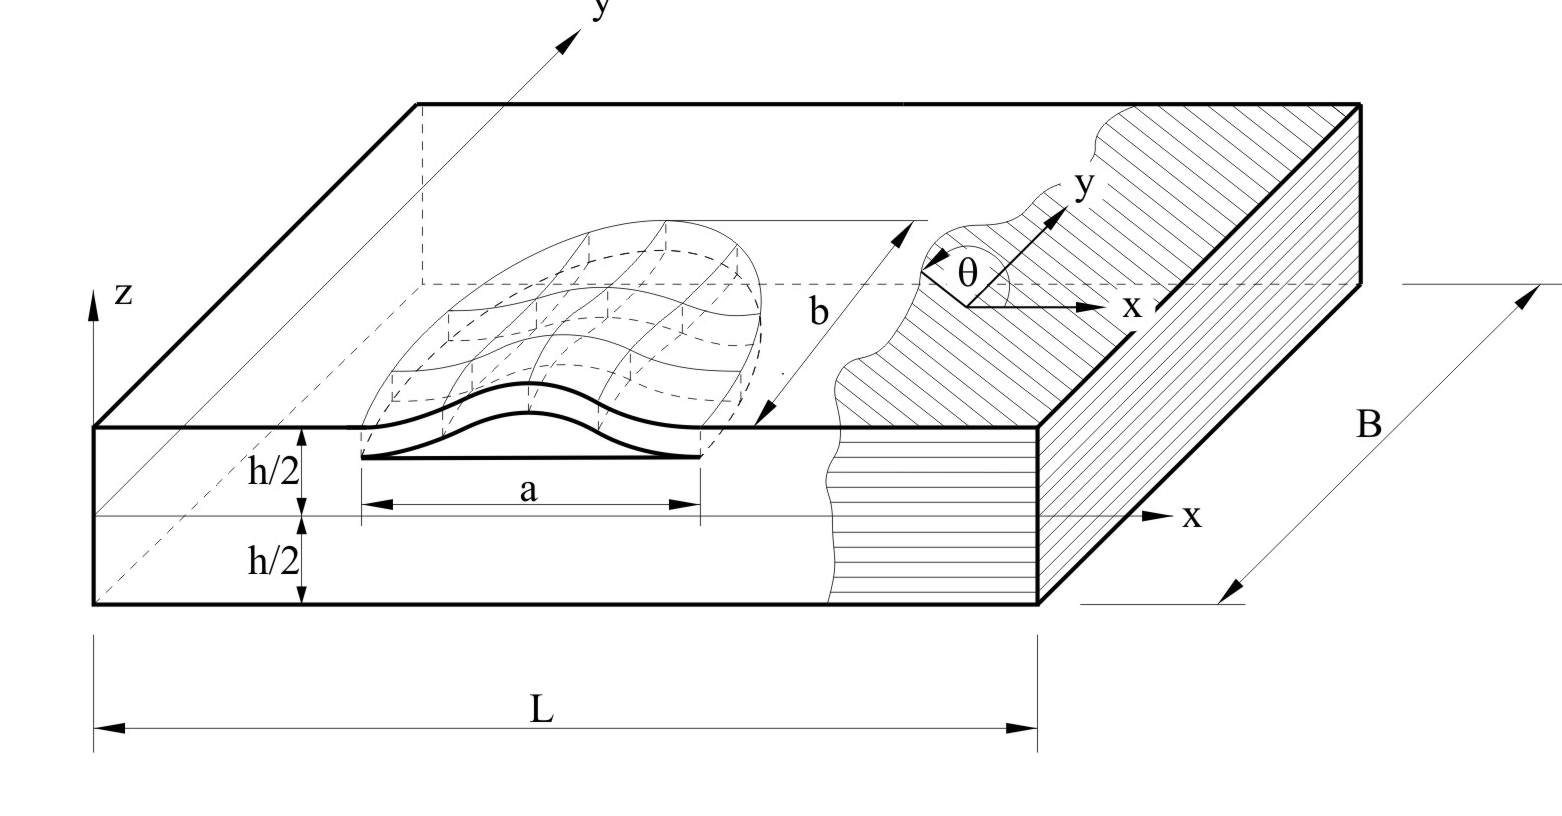
\includegraphics[width=.95\textwidth]{delaminated_plate1.jpg}
%				\end{figure}
%			\end{column}
%		\end{columns}
%	\end{frame}
%	%%%%%%%%%%%%%%%%%%%%%%%%%%%%%%%%%%%%%%%%%%%%%%%%%%%%%%%%%%%%%%%%%%%%%%%%%%%%
%	\note{
%		Composite laminates have a wide range of applications in various industries due to their characteristics, such as high strength, low density, and resistance to fatigue and corrosion, among others.
%		
%		However, defects such as cracks, fibre breakage, and debonding can occur in composite laminates. 
%		
%		In particular, laminated composite materials are more sensitive to damage in the form of delamination due to weak transverse tensile and interlaminar shear strengths.
%			
%		Delaminations can seriously decrease the performance of composite structures.
%		Accordingly, delamination detection in its early stages can significantly help to avoid catastrophic structural collapses.		
%	}
%	%%%%%%%%%%%%%%%%%%%%%%%%%%%%%%%%%%%%%%%%%%%%%%%%%%%%%%%%%%%%%%%%%%%%%%%%%%%%
%	\section{Objectives}
%	\begin{frame}{Objectives}
%		\textbf{To develop \textcolor{blue}{a novel AI-driven diagnostic system} for delamination identification in composite laminates such as carbon fibre reinforced polymers (CFRP).}
%		\vfil
%		\textbf{To address the issue of \textcolor{blue}{slow data acquisition} by SLDV of high-resolution full wavefields of Lamb wave propagation.}
%		\begin{alertblock}{Thesis}
%			It is possible to use an end-to-end approach in which DNN 
%			processes the animation of propagating waves (input) directly into a damage map (output).
%		\end{alertblock}
%	\end{frame}
%	%%%%%%%%%%%%%%%%%%%%%%%%%%%%%%%%%%%%%%%%%%%%%%%%%%%%%%%%%%%%%%%%%%%%%%%%%%%%
%	\note{
%		The main objective of this work is to develop an artificial intelligence-based diagnostic system for the detection of delaminations in composite laminates.
%		
%		Therefore, I investigated the possibility of embracing the end-to-end approach by using animations of Lamb wave propagation in a plate interacting with discontinuities such as damage and edges with an artificial intelligence-based approach to detect and identify delaminations.
%		
%		My second objective is to address the issue of slow data acquisition of high-resolution full wavefields of Lamb wave propagation by SLDV. 		
%	}
%	%%%%%%%%%%%%%%%%%%%%%%%%%%%%%%%%%%%%%%%%%%%%%%%%%%%%%%%%%%%%%%%%%%%%%%%%%%%%
	\section{Introduction to SHM/NDT}
	%%%%%%%%%%%%%%%%%%%%%%%%%%%%%%%%%%%%%%%%%%%%%%%%%%%%%%%%%%%%%%%%%%%%%%%%%%%%
	\begin{frame}{Structural Health Monitoring (SHM)}
		\begin{columns}[T]
			\begin{column}[c]{0.3\textwidth}
				\justifying
				Structural Health Monitoring (SHM) refers to the process of continuously monitoring and evaluating the condition of structures to ensure their safety and performance.
			\end{column}
			\begin{column}[c]{.6\textwidth}
				\begin{figure}
					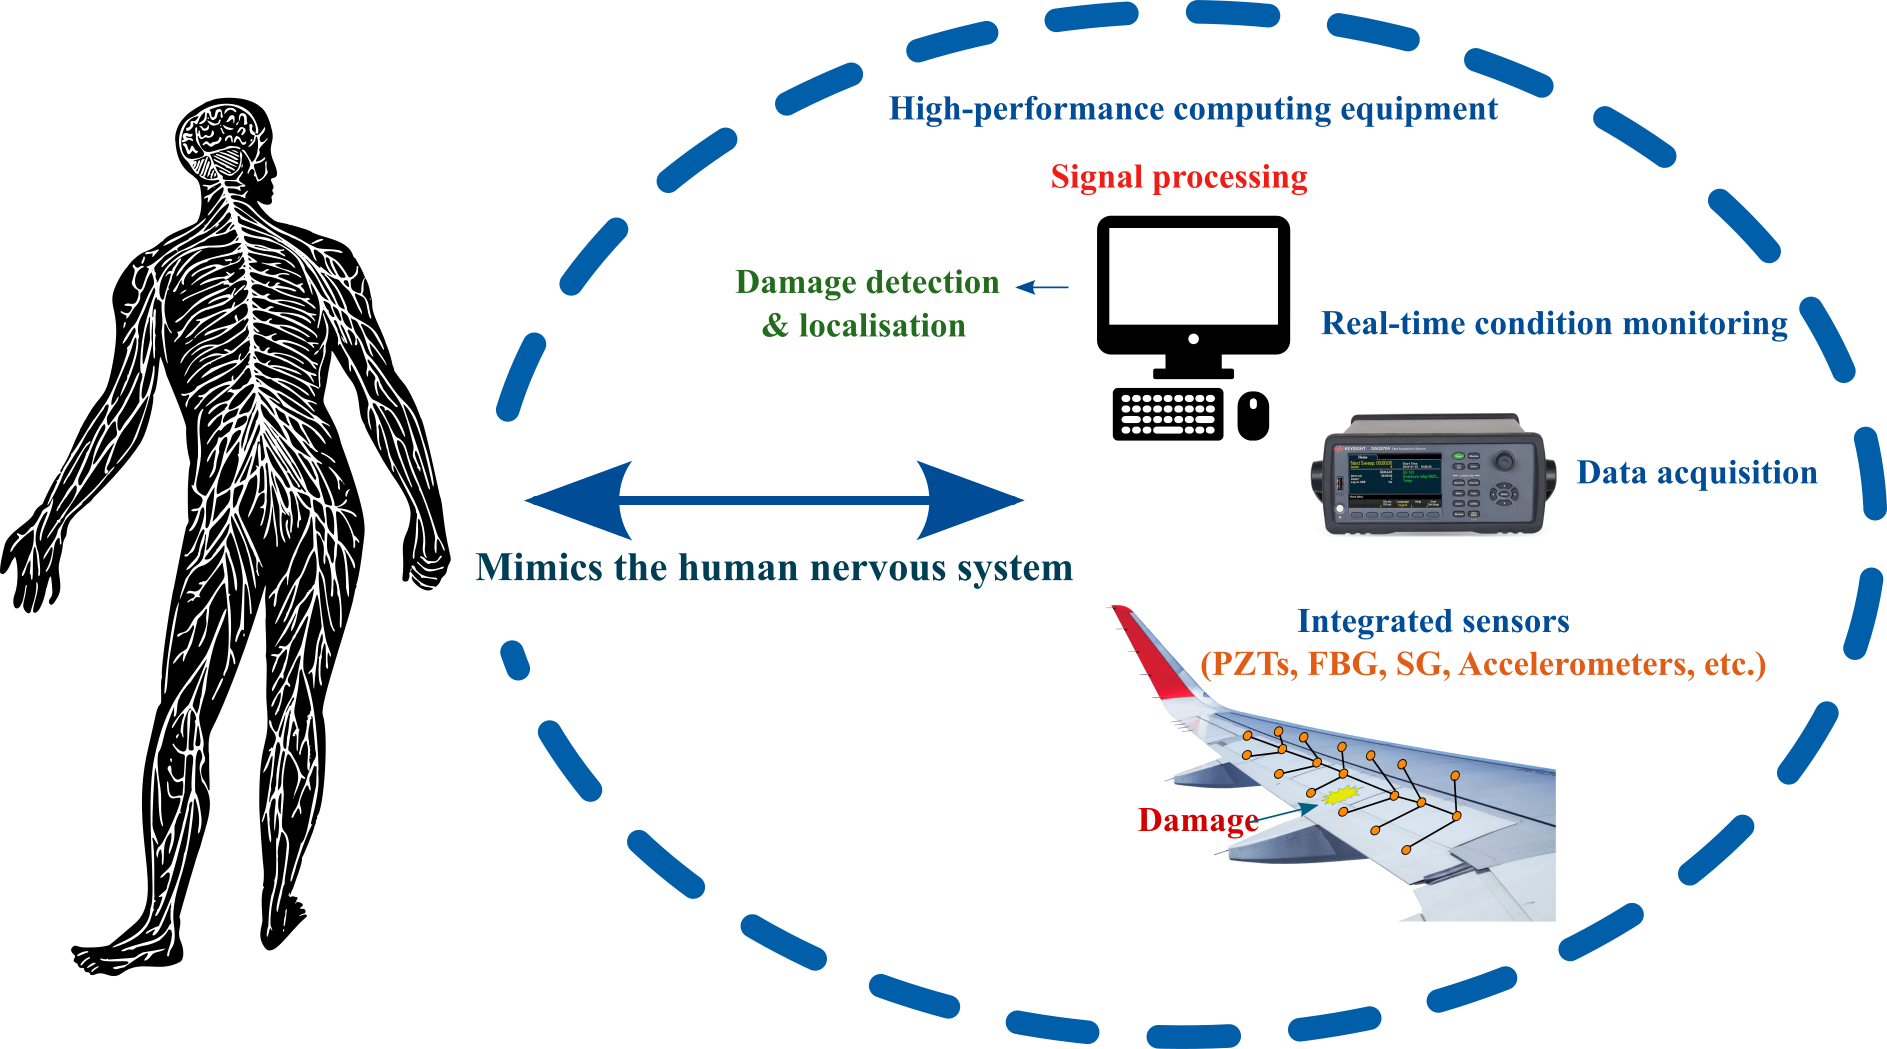
\includegraphics[height=.6\textwidth]{SHM_system.png}
				\end{figure}
			\end{column}
		\end{columns}
	\end{frame}
	%%%%%%%%%%%%%%%%%%%%%%%%%%%%%%%%%%%%%%%%%%%%%%%%%%%%%%%%
	\note{
		Structural health monitoring is about monitoring a structure periodically or continuously to evaluate its technical conditions.
		
		As a result, the SHM aims to place integrated sensors on the structure to continuously monitor its condition.
		
		In this way, structural health monitoring mimics the human nervous system, which can provide us with real-time readings and detect any abnormal events.
		
		Accordingly, this is the ultimate aim of SHM: to monitor in real-time in a way that can detect damage early so we can perform preventive measures to protect the structure.
	}
	%%%%%%%%%%%%%%%%%%%%%%%%%%%%%%%%%%%%%%%%%%%%%%%%%%%%%%%%
	\begin{frame}{Non-destructive testing (NDT)}
		\begin{columns}[T]
			\begin{column}{.35\textwidth}
				\justifying
				NDT techniques are used to inspect materials, components, and structures without causing permanent damage or altering their integrity. 
			\end{column}
			\begin{column}{.65\textwidth}
				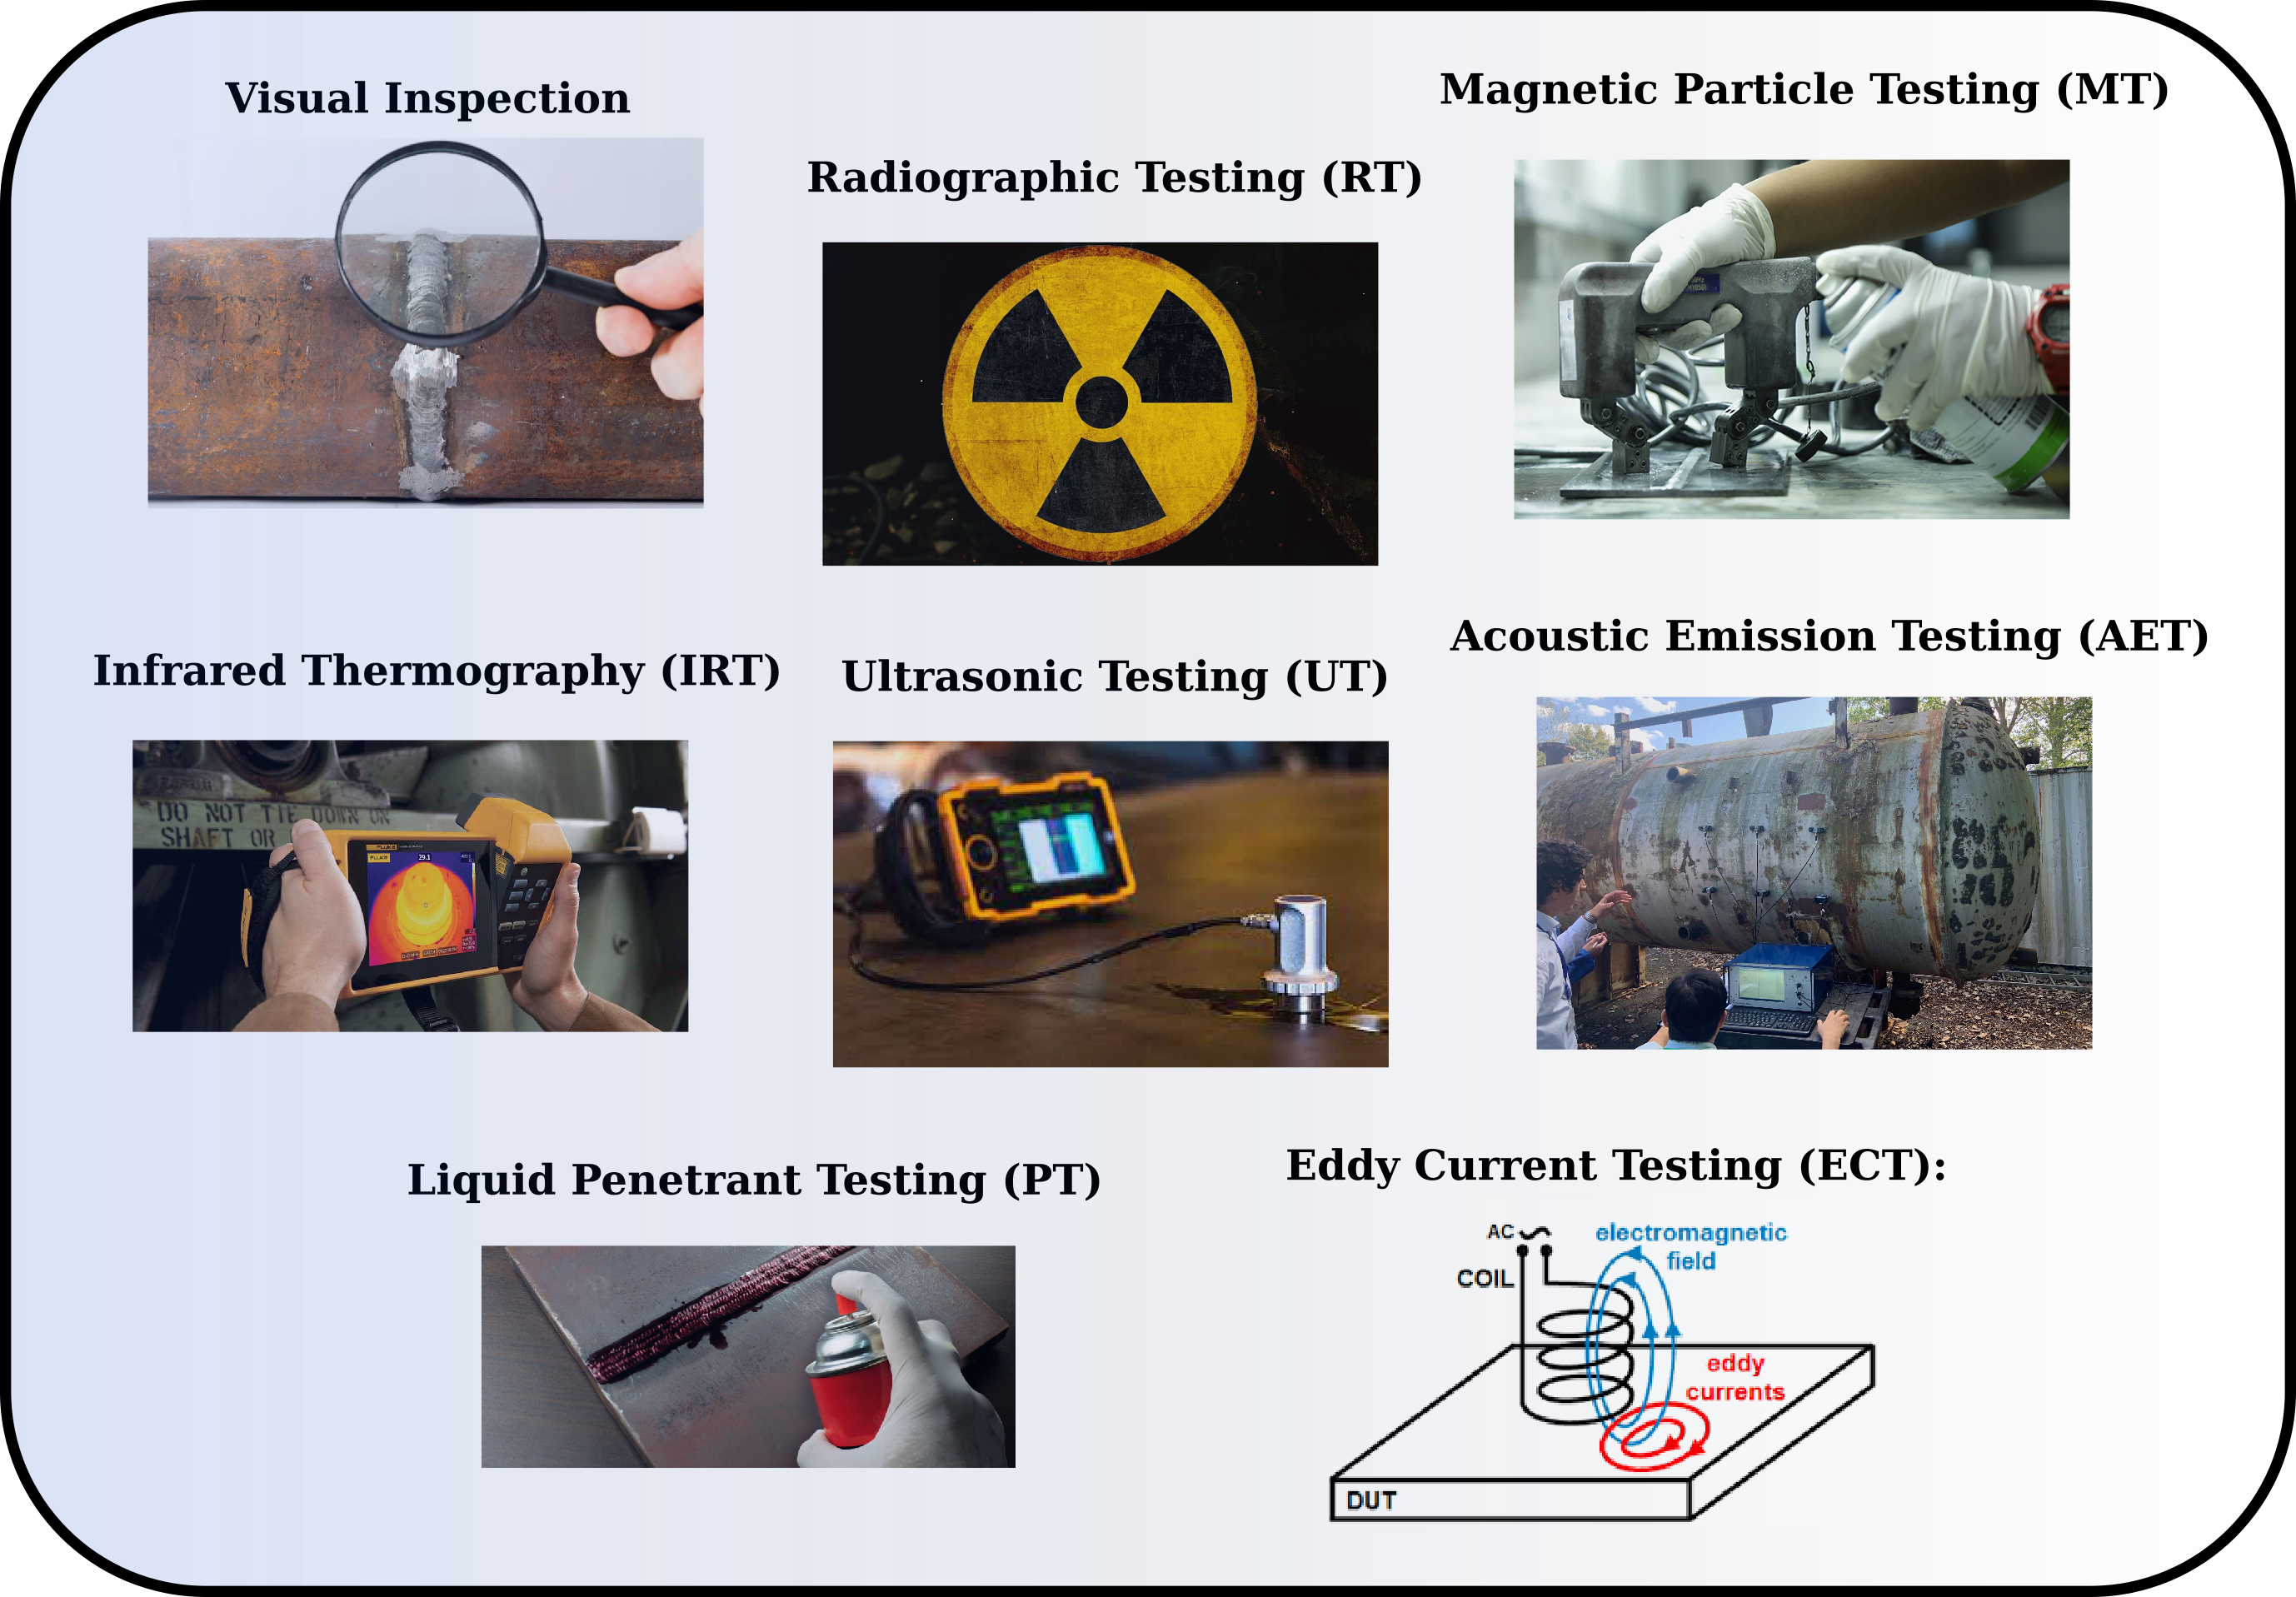
\includegraphics[width=0.95\textwidth]{NDT.png}
			\end{column}
		\end{columns}
	\end{frame}
	%%%%%%%%%%%%%%%%%%%%%%%%%%%%%%%%%%%%%%%%%%%%%%%%%%%%%%%%
	\note{
		NDT techniques are used to inspect materials, components, and structures without causing permanent damage or altering their integrity. 
		These techniques are employed across various industries to ensure the quality, reliability, and safety of products and infrastructure. Some common non-destructive testing techniques include:
		
		Visual Inspection: The simplest and most widely used technique, involving direct visual examination to identify surface defects, cracks, corrosion, or other abnormalities.
		
		Ultrasonic Testing (UT): Utilizes high-frequency sound waves to detect internal flaws or changes in material properties. Ultrasonic waves are directed into the test object, and the reflections or changes in the waves are analysed to identify defects.
		
		Radiographic Testing (RT): Involves the use of X-rays, gamma rays, or other penetrating radiation to inspect internal structures or welds. The radiation passes through the object, and the resulting image reveals any defects or inconsistencies.
		
		Magnetic Particle Testing (MT): Detects surface or near-surface defects in ferromagnetic materials. The material is magnetized, and magnetic particles are applied to the surface. The particles accumulate at defect locations, making them visible for inspection.
		
		Liquid Penetrant Testing (PT): A surface inspection method where a liquid dye or fluorescent penetrant is applied to the material. The penetrant seeps into surface cracks or flaws, and excess penetrant is removed. A developer is then applied, highlighting any defects through dye bleeding or fluorescence.
		
		Eddy Current Testing (ECT): Primarily used for conductive materials, this technique utilizes electromagnetic induction to detect flaws or changes in electrical conductivity. Eddy currents are induced in the material, and variations in the electrical response are analysed for defect identification.
		
		Acoustic Emission Testing (AET): Monitors acoustic signals emitted by a material during stress or deformation. It is useful for detecting active defects or ongoing damage in structures under load.
		
		Infrared Thermography (IRT): Utilizes thermal imaging cameras to detect and analyse thermal patterns on the surface of an object. It helps identify anomalies, such as heat loss, hotspots, or defects, by detecting variations in temperature.
		
				
		These techniques, among others, are chosen based on the material, the type of defect or inspection required, and the specific industry standards and regulations in place. 
		Each method has its strengths and limitations, and NDT professionals select the appropriate technique or combination of techniques to ensure accurate and reliable inspection results.
		
	}
	%%%%%%%%%%%%%%%%%%%%
	\begin{frame}{Ultrasonic testing (UT)} 
		\begin{columns}[T]
			\begin{column}[c]{0.38\textwidth}
				\textbf{Ultrasonic waves}	
				\begin{itemize}
					\item Frequency range: 2 MHz - 200 MHz
					\item Wavelength \(\lambda << h\) thickness 
					\item shorter wavelengths
				\end{itemize}
				\textbf{Guided waves}	
				\begin{itemize}
					\item Typical frequency range: \\ 10 kHz - 1 MHz
					\item Wavelength \(\lambda > h\) thickness 
					\item longer wavelengths
				\end{itemize}
			\end{column}
			\begin{column}[c]{0.6\textwidth}				
				\textbf{Ultrasonic testing} \hspace{50pt} \textbf{Guided wave testing}
				\begin{figure}
					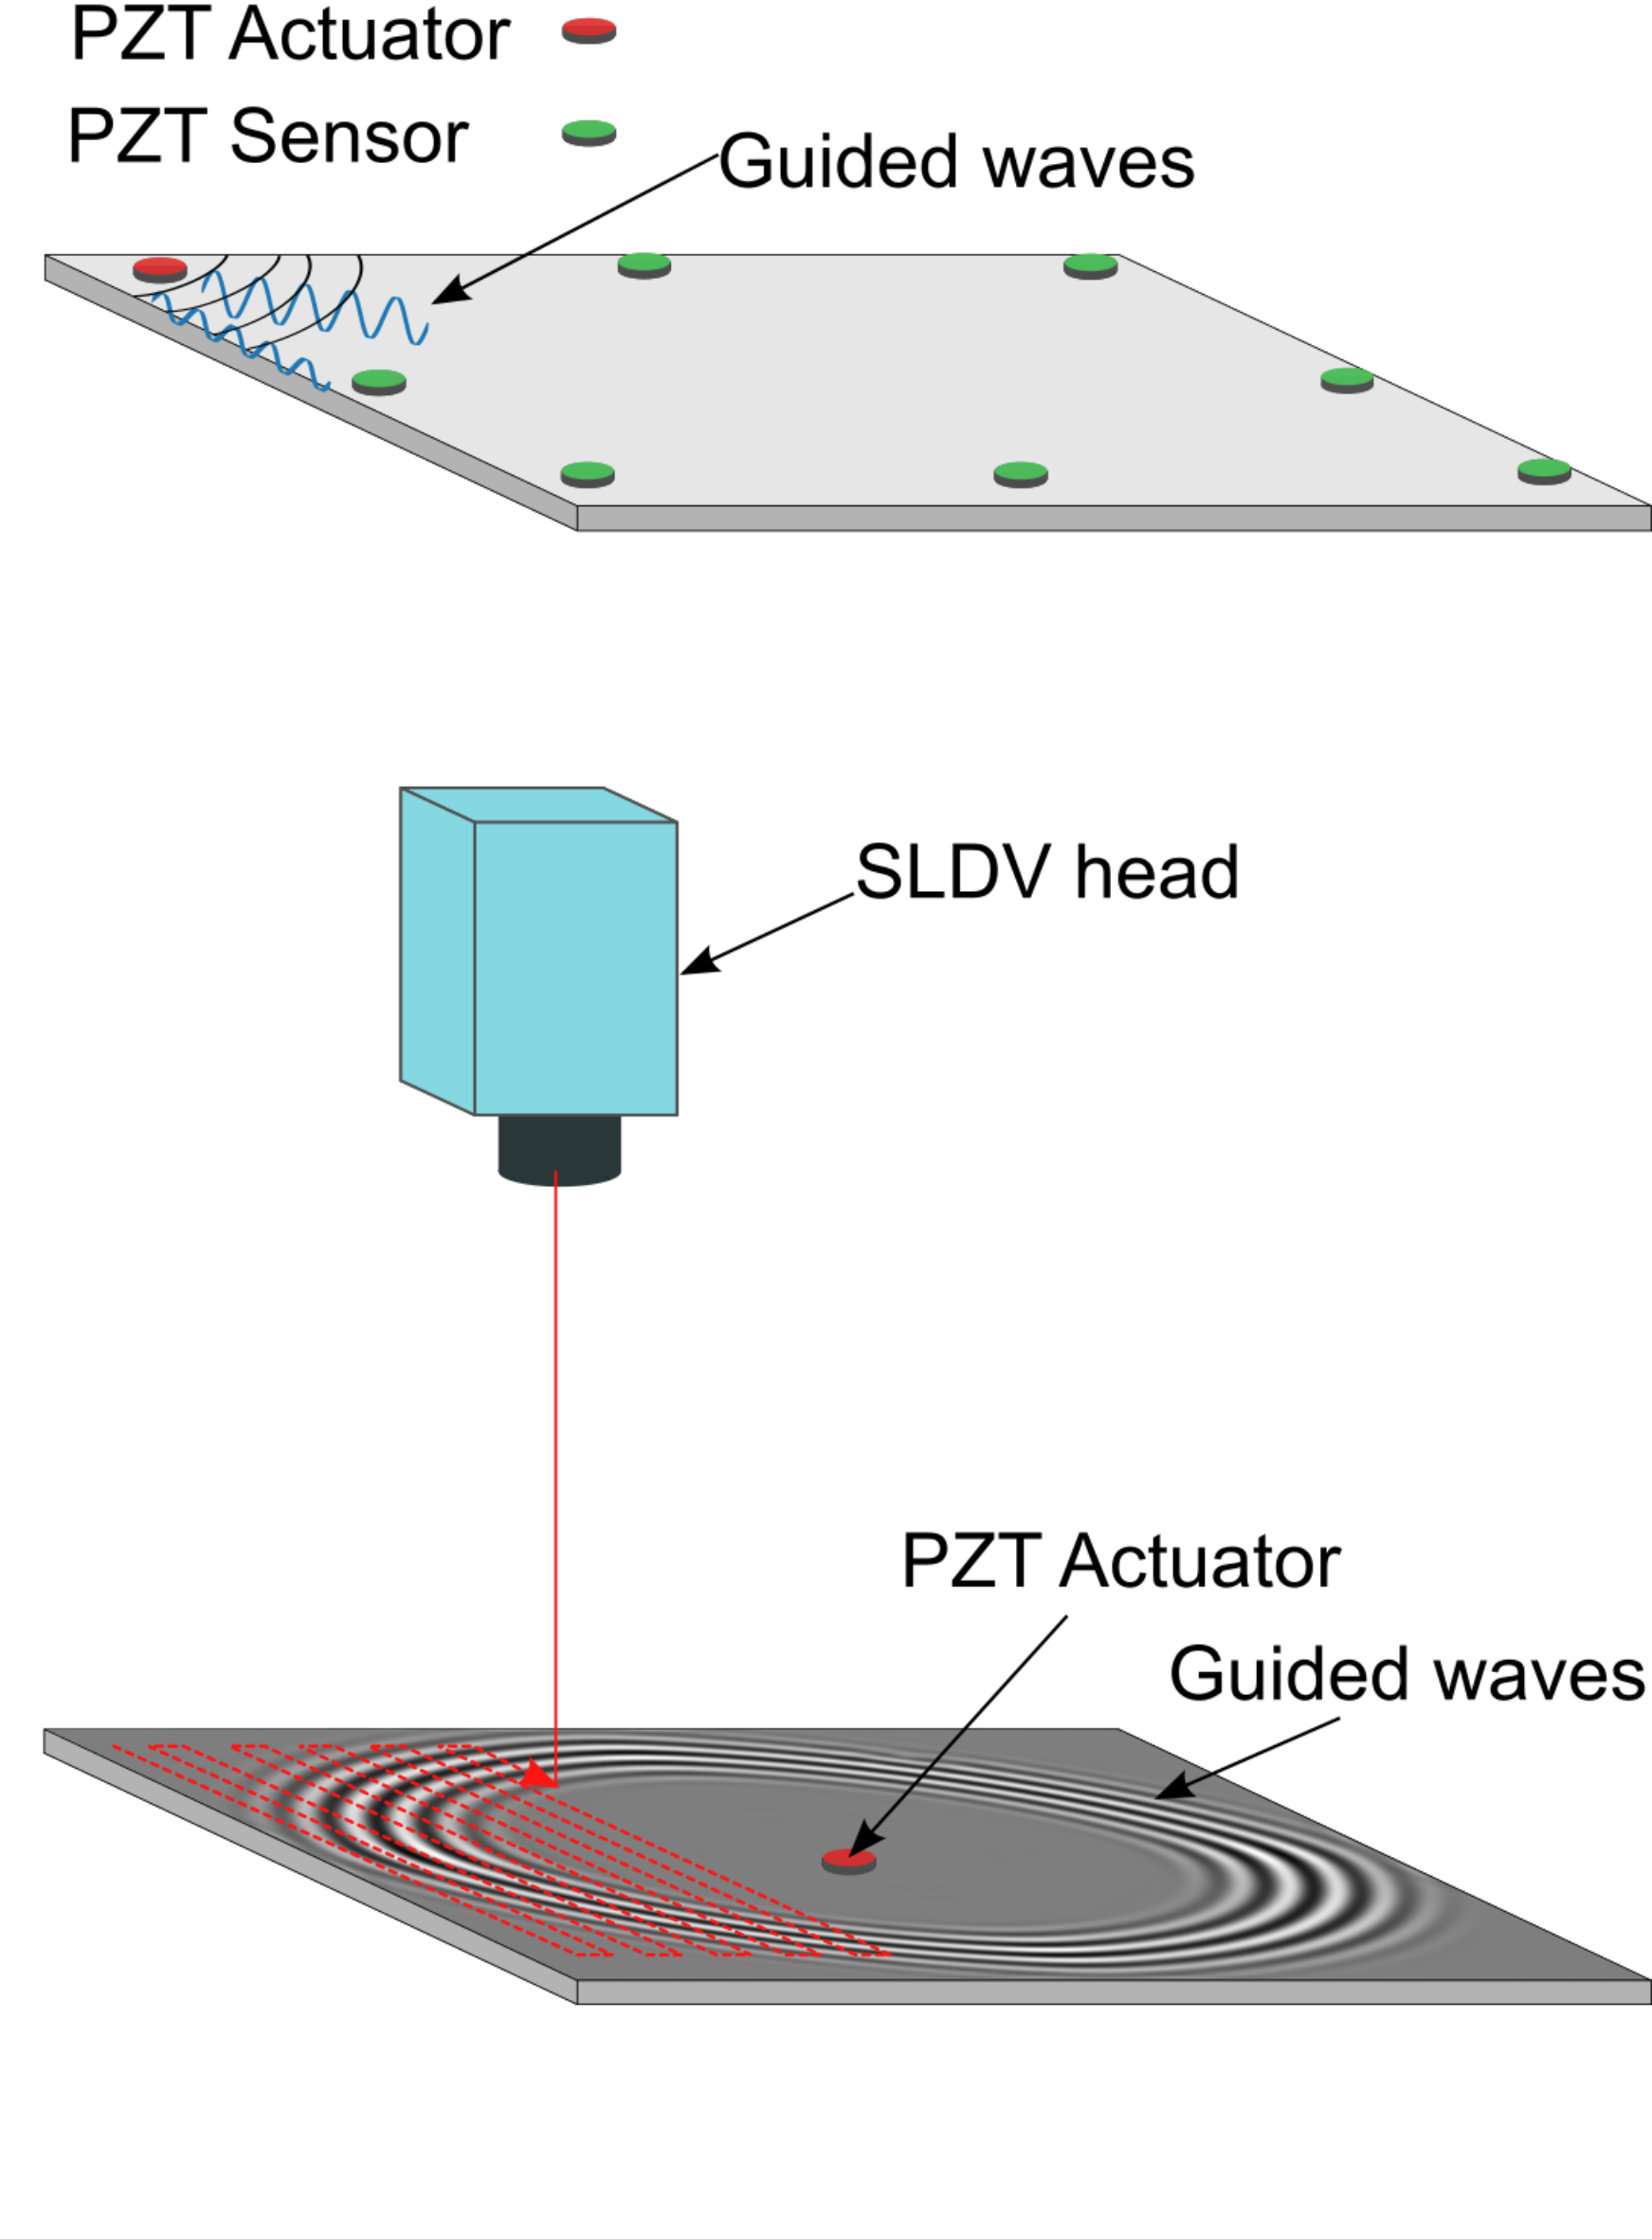
\includegraphics[width=0.95\textwidth]{local_ultrasonic.png}
				\end{figure}
			\end{column}		
		\end{columns}	
	\end{frame}
	\note{
		\tiny
		Many conventional methods have been used for a long time in the industry for damage inspection, such as visual inspection, Eddy current, dye penetration, acoustic emission, and local ultrasonic testing.
		For the local ultrasonic testing, the frequency is in the range of 2 MHz–200 MHz, and the wavelength is way smaller than the thickness of the structure.
		There are different methods for ultrasonic testing, such as:
		pulse echo, in which we have a probe that generates ultrasonic waves that propagate through the thickness of a structure, and then the reflected waves from the bottom surface are captured by the same probe.
		The other ultrasonic method is called the "through-transmission method."
		There are two probes: one for transmitting on one side and the other for receiving on the other side.
		As a result, these methods are local, but they have some drawbacks:
		Labor-intensive, time-consuming, professional, and experienced personnel are required; complex structures may need to be disassembled.
		On the other hand, guided wave testing is a promising global NDE solution for SHM.
		The typical frequency range of guided waves is 10 kHz to 1 MHz, and their wavelength is larger than the thickness of the investigated structure.
		Guided waves can be generated using a piezoelectric actuator and registered by an array of piezoelectric sensors. 
		Alternatively, the propagation of guided Lamb waves can be registered using a scanning laser Doppler vibrometer to produce a full wavefield scan.		 
	}
	%%%%%%%%%%%%%%%%%%%%%%%%%%%%%%%%%%%%%%%%%%%%%%%%%%%%%%%%
	\section{Guided waves}
	%%%%%%%%%%%%%%%%%%%%%%%%%%%%%%%%%%%%%%%%%%%%%%%%%%%%%%%%
	\begin{frame}{Waves used in non-destructive testing}
		%%%%%%%%%%%%%%%%%%%%%%%%%%%%%%%%%%%%%%%%%%%%%%%%%%%%
		Elastic wave propagation types depending on particle motion:
		\begin{itemize}
				\item  \alert{The longitudinal wave} is a compressional wave in which the particle motion is in the same direction as the propagation of the wave
				\item \alert{The shear wave} is a wave motion in which the particle motion is perpendicular to the direction of the propagation
				\item \alert{Surface (Rayleigh) waves} have an elliptical particle motion and travel across the surface of a material. Their velocity is approximately 90\% of the shear wave velocity of the material and their depth of penetration is approximately equal to one
				wavelength
				\item \alert{Plate (Lamb) waves} have a complex vibration occurring in materials where thickness is less than the wavelength of elastic wave introduced into it.
			\end{itemize}
	\end{frame}
	%%%%%%%%%%%%%%%%%%%%%%%%%%%%%%%%%%%%%%%%%%%%%%%%%%%%%%%%
	\setcounter{subfigure}{0}
	\begin{frame}{Waves used in non-destructive testing}
	%%%%%%%%%%%%%%%%%%%%%%%%%%%%%%%%%%%%%%%%%%%%%%%%%%%
		\begin{figure}
				\subfloat{\animategraphics[autoplay,loop, controls,width=0.5\textwidth]{10}{figures/gif_figs/Longitudinal_wave/Longitudinal_wave-}{0}{35}}
				\caption{\alert{Longitudinal wave} - plane pressure pulse wave}
			\end{figure}
	\tiny 
	(source: https://nojigon.webs.upv.es/index.php)
	\end{frame}
	%%%%%%%%%%%%%%%%%%%%%%%%%%%%%%%%%%%%%%%%%%%%%%%%%%%%%%%%%%%%%%%%%%%%%%%%%%%%%%%%%
	%%%%%%%%%%%%%%%%%%%%%%%%%%%%%%%%%%%%%%%%%%%%%%%%%%%
	\setcounter{subfigure}{0}
	\begin{frame}{Waves used in non-destructive testing}
		%%%%%%%%%%%%%%%%%%%%%%%%%%%%%%%%%%%%%%%%%%%%%%%%%%
		\begin{columns}[T]
				\begin{column}{0.5\textwidth}
						\centering
						\begin{figure}
								\subfloat{\animategraphics[autoplay,loop, controls,width=0.95\textwidth]{10}{figures/gif_figs/SH_shear_wave/SH_shear-}{0}{39}}
								\caption{\alert{Shear horizontal wave}}
							\end{figure}			
					\end{column}
				\begin{column}{0.5\textwidth}
						\centering
						\begin{figure}
								\subfloat{\animategraphics[autoplay,loop, controls,width=0.95\textwidth]{10}{figures/gif_figs/SV_shear_wave/SV_shear-}{0}{39}}
								\caption{\alert{Shear vertical wave}}
							\end{figure}			
					\end{column}	
			\end{columns}
	\tiny 
	(source: https://nojigon.webs.upv.es/index.php)
	\end{frame}
	%%%%%%%%%%%%%%%%%%%%%%%%%%%%%%%%%%%%%%%%%%%%%%%%%%%
	\setcounter{subfigure}{0}
	\begin{frame}{Waves used in non-destructive testing}
		%%%%%%%%%%%%%%%%%%%%%%%%%%%%%%%%%%%%%%%%%%%%%%%%%%
		\begin{figure}
				\centering
				\subfloat{\animategraphics[autoplay,loop, controls,height=0.65\textheight]{15}{figures/gif_figs/Raileigh_wave/Raileigh_wave-}{0}{67}}
				\caption{\alert{Rayleigh waves}}		
			\end{figure}			
	\tiny 
	(source: https://nojigon.webs.upv.es/index.php)
	\end{frame}
	%%%%%%%%%%%%%%%%%%%%%%%%%%%%%%%%%%%%%%%%%%%%%%
	\setcounter{subfigure}{0}
	\begin{frame}{Waves used in non-destructive testing}
		%%%%%%%%%%%%%%%%%%%%%%%%%%%%%%%%%%%%%%%%%%%%%%
		\begin{figure}			
				\centering
				\subfloat{\animategraphics[autoplay,loop, controls,height=0.65\textheight]{20}{figures/gif_figs/love_wave/love_wave-}{0}{107}}
				\caption{\alert{Love waves} (surface seismic waves) named after Augustus Edward Hough Love}		
			\end{figure}			
	\tiny 
	(source: https://nojigon.webs.upv.es/index.php)
	\end{frame}
	%%%%%%%%%%%%%%%%%%%%%%%%%%%%%%%%%%%%%%%%%%%%%
	\setcounter{subfigure}{0}
	\begin{frame}{Lamb waves}
		%%%%%%%%%%%%%%%%%%%%%%%%%%%%%%%%%%%%%%%%%%%%%%
		\begin{alertblock}{Lamb waves}	
			Lamb waves are plane waves propagating in thin plates.\\
			Shear vertical waves in conjunction with longitudinal P waves interacts with plate surfaces resulting in complex wave mechanism which leads to creation of Lamb waves.
		\end{alertblock}
%		Horace Lamb discovered these type of waves in 1917.
%		He derived theory and dispersion relations.
		\begin{columns}[T]
			\begin{column}{0.5\textwidth}
				\centering
				symmetric modes
				\begin{equation*}
					\frac{\tan(q h)}{\tan(p h)} = -\frac{4 k^2 p q}{\left(q^2 - k^2\right)^2}
				\end{equation*}
			\end{column}
			\begin{column}{0.5\textwidth}
				\centering
				antisymmetric modes
				\begin{equation*}
					\frac{\tan(q h)}{\tan(p h)} = -\frac{\left(q^2 - k^2\right)^2}{4 k^2 p q}
				\end{equation*}
			\end{column}	
		\end{columns}	
		\centering
%		\(q=q(\omega,k), \quad p=p(\omega,k) \)
		\begin{gather*}
			\centering
			p^2 = \frac{\omega^2}{c_{L}^2}-k^2,\ q^2 = \frac{\omega^2}{c_{S}^2}-k^2,\ k = \frac{2\pi}{\lambda},\ f=\frac{\omega}{2\pi}
		\end{gather*}
		\newline
		\begin{gather*}
			\centering
			c_L=\sqrt{\frac{2\mu (1-\nu)}{\rho(1-2\nu)}},\ c_S=\sqrt{\frac{\mu}{\rho}}
		\end{gather*}
	\end{frame}
	%%%%%%%%%%%%%%%%%%%%%%%%%%%%%%%%%%%%%%%%%%%%%%%%%%%%%%%%%%%%%%%%%%%%%%%%%%%%
	\note{
		Lamb waves are a subset of guided waves that propagate between two parallel surfaces, such as in shell and plate structures discovered by Horace Lamb in 1917.
		
		Lamb waves can be separated into symmetric modes and antisymmetric modes in terms of the surface particle motion to the mid-plane, which are described in characteristic Lamb wave equations:
		
		
		where $h$ is the half-thickness of the plate, $k$ is the wavenumber, $\omega$ is the angular frequency, and $\lambda$ is the wavelength. 
		\(cL\) and \(cS\) are the velocities of longitudinal and transverse
		waves, respectively.
		
		where \(\rho\) is the density, \(\mu\) is the shear modulus, and \(\nu\) is Poisson's ratio of the medium.
	}
	%%%%%%%%%%%%%%%%%%%%%%%%%%%%%%%%%%%%%%%%%%%%%%%%%%%%%%%%%%%%%%%%%%%%%%%%%%%%
	\setcounter{subfigure}{0}
	\begin{frame}{Lamb waves modes}
		%%%%%%%%%%%%%%%%%%%%%%%%%%%%%%%%%%%%%%%%%%%%%%
		\begin{columns}[T]
			\begin{column}{0.3\textwidth}
				\centering
				\begin{figure}
					\animategraphics[autoplay,loop,width=1\textwidth]{10}{figures/gif_figs/S0_mode/S0_mode-}{0}{67}
					\caption{Fundamental symmetric, S0, \alert{Lamb wave} mode (in-plane motion)}
				\end{figure}
			\end{column}
			\begin{column}{0.3\textwidth}
				\centering
				\begin{figure}
					\animategraphics[autoplay,loop,width=1\textwidth]{10}{figures/gif_figs/A0_mode/A0_mode-}{0}{67}
					\caption{Fundamental antisymmetric, A0, \alert{Lamb wave} mode (out-of-plane motion)}
				\end{figure}
			\end{column}
			\hfill
			\begin{column}{0.37\textwidth}
					\begin{itemize}
						\item \textcolor{blue}{Travel within guides for long distances}
						\item \textcolor{blue}{Can propagate in complex structures}
%						\item \textcolor{blue}{High speeds in metals and composites}
						\item \textcolor{blue}{Can be automated using software}
					\end{itemize}
					\textbf{Lamb waves are a promising global NDE solution for SHM}
			\end{column}
		\end{columns}	
		\tiny 
		(source: https://nojigon.webs.upv.es/index.php)
	\end{frame}
	%%%%%%%%%%%%%%%%%%%%%%%%%%%%%%%%%%%%%%%%%%%%%%%%%%%%%%%%%%%%%%%%%%%%%%%%%%%%
	\note{
		The animation on the left shows the fundamental symmetric \(S_0\) mode of the Lamb wave.
		
		We can see the in-plane motion of the particles.
		Whereas the second animation shows the fundamental antisymmetric \(A_0\) mode of the Lamb wave.
		We can see the out-of-plane motion of the particles.
		
		Furthermore, Lamb wave has some good characteristics that make it a promising solution for SHM as it:\\
		1. Can travel within guides for long distances. \\
		2. Can propagate in complex structures. \\
%		3. Has high speed in metals and composites.\\ 	
	}
	%%%%%%%%%%%%%%%%%%%%%%%%%%%%%%%%%%%%%%%%%%%%%%%%%%%%%%%%%%%%%%%%%%%%%%%%%%%%
	
%	\begin{frame}{Dispersion curves of Lamb waves}
%		%%%%%%%%%%%%%%%%%%%%%%%%%%%%%%%%%%%%%%%%%%%%%%
%		\begin{figure}
%			\only<1>{
%				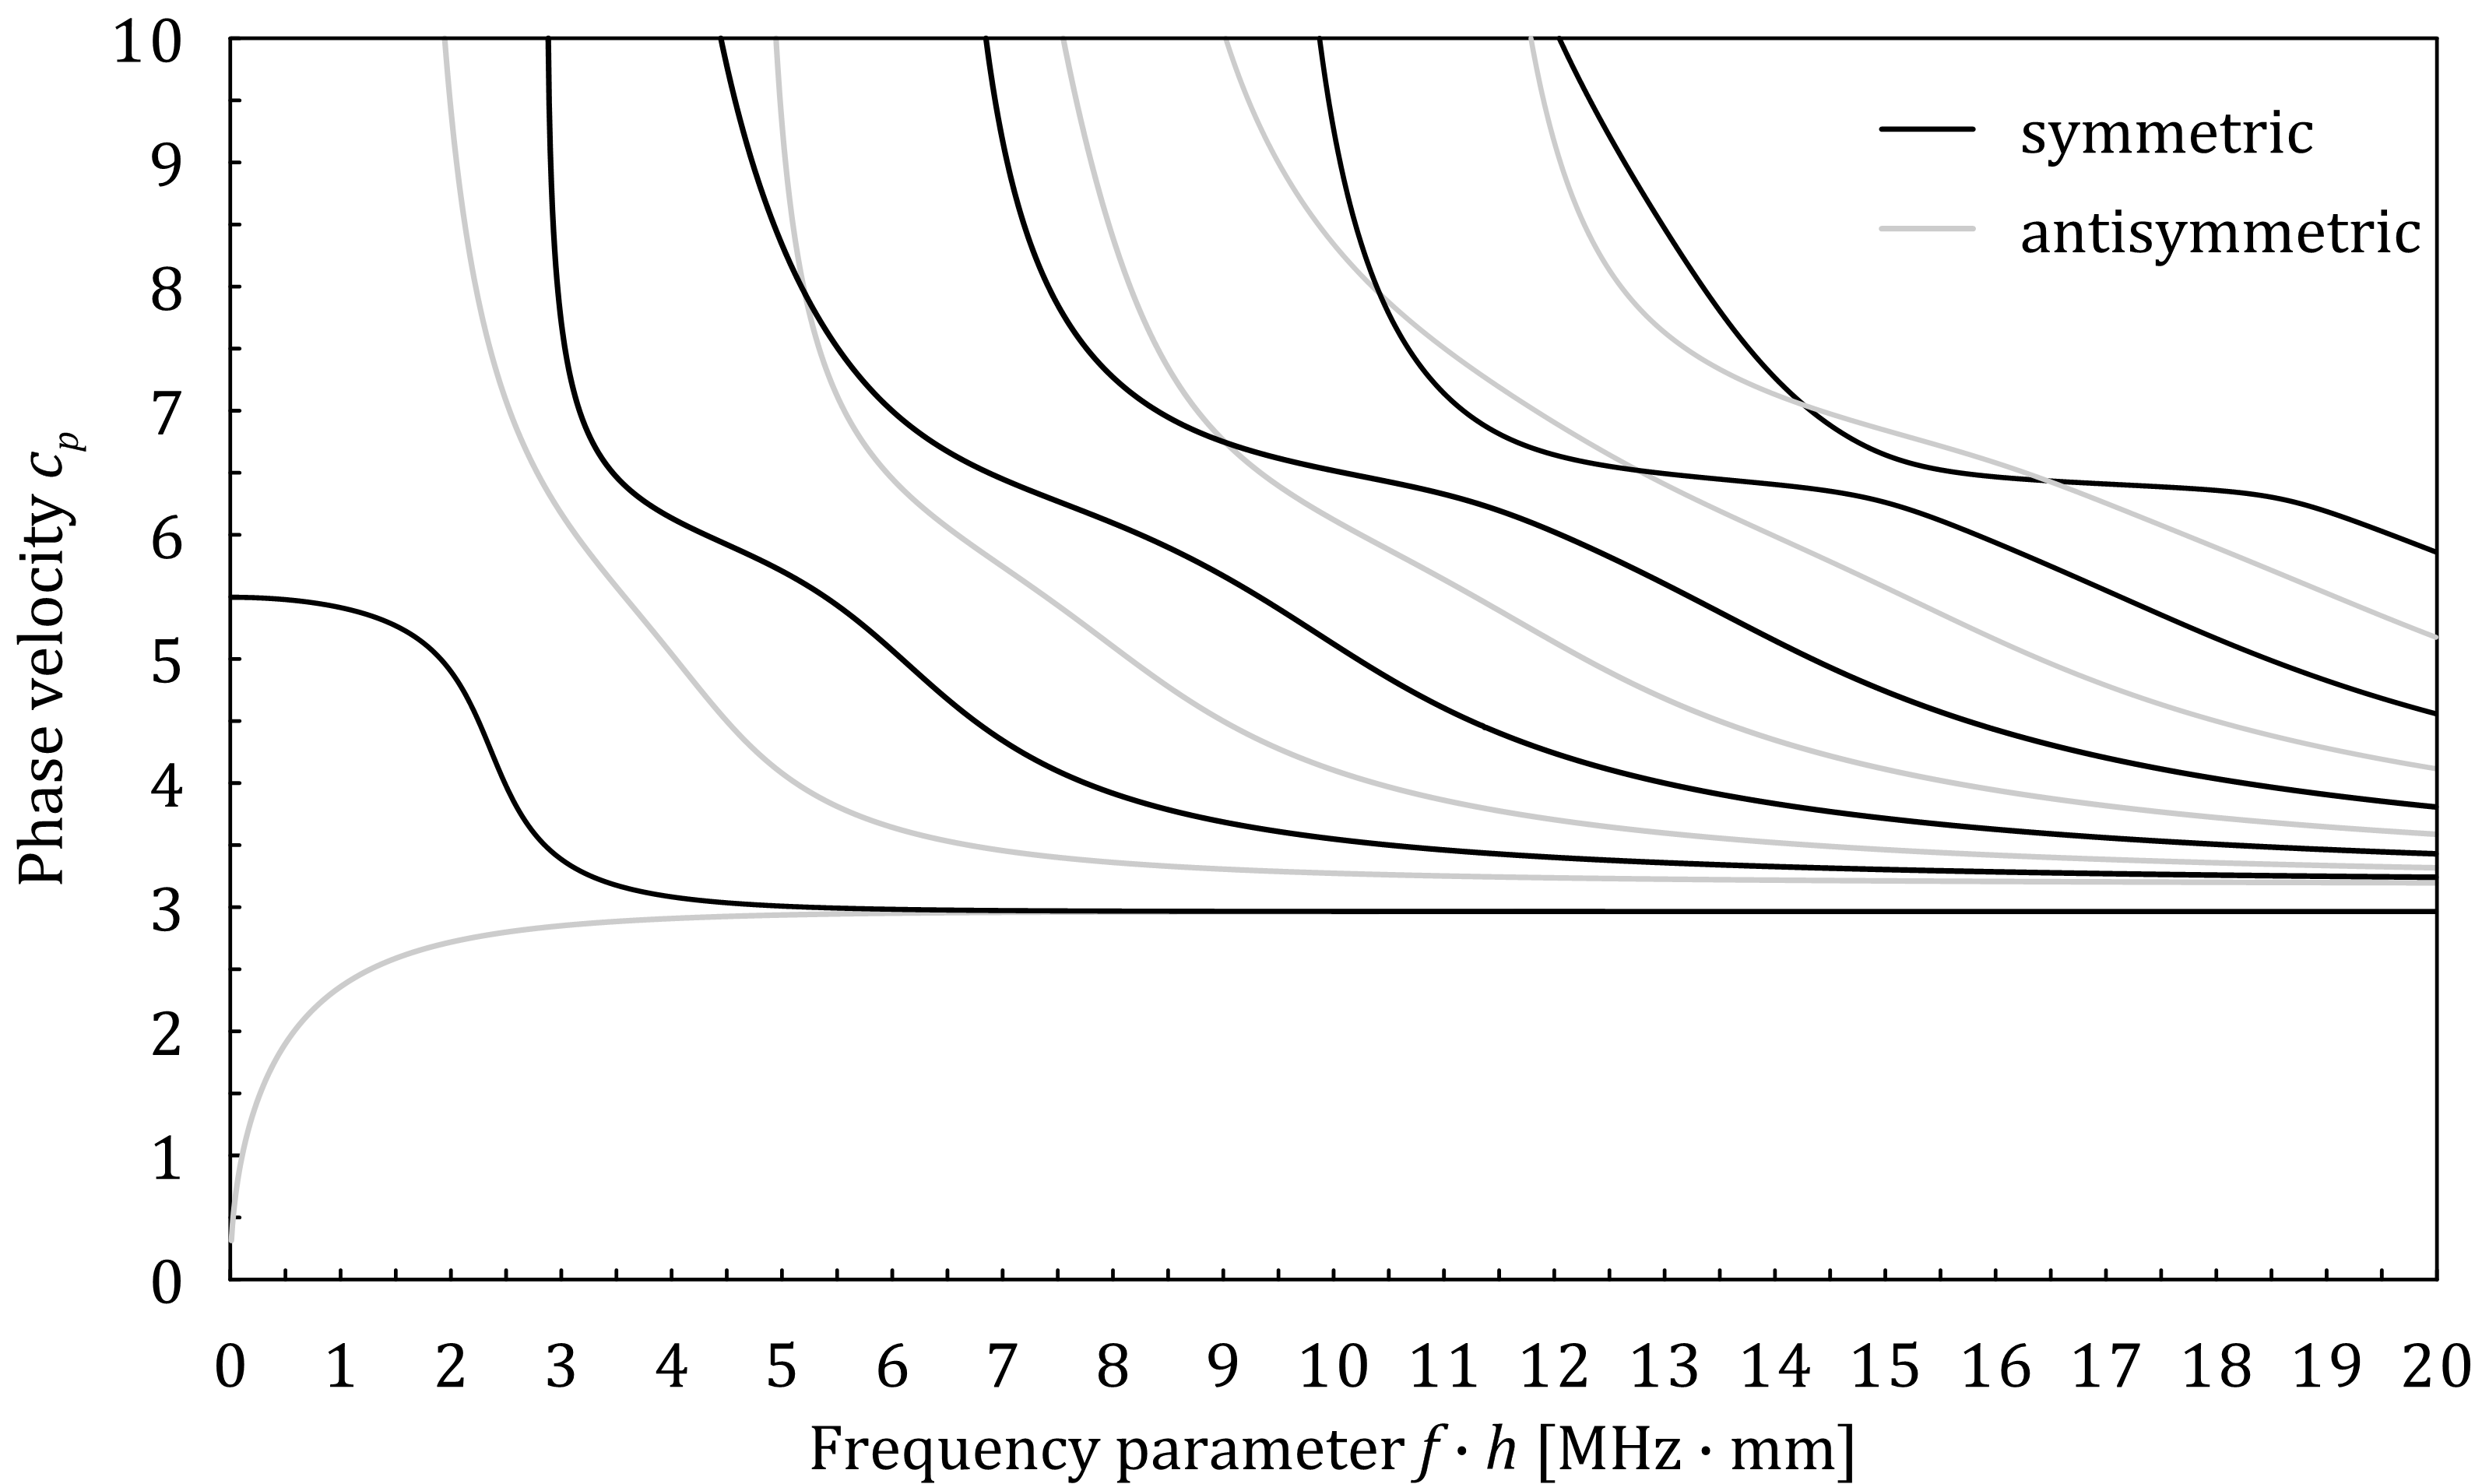
\includegraphics[width=0.8\textwidth]{/figs/Fig_1_12.png}	
%			}
%			\only<2>{
%				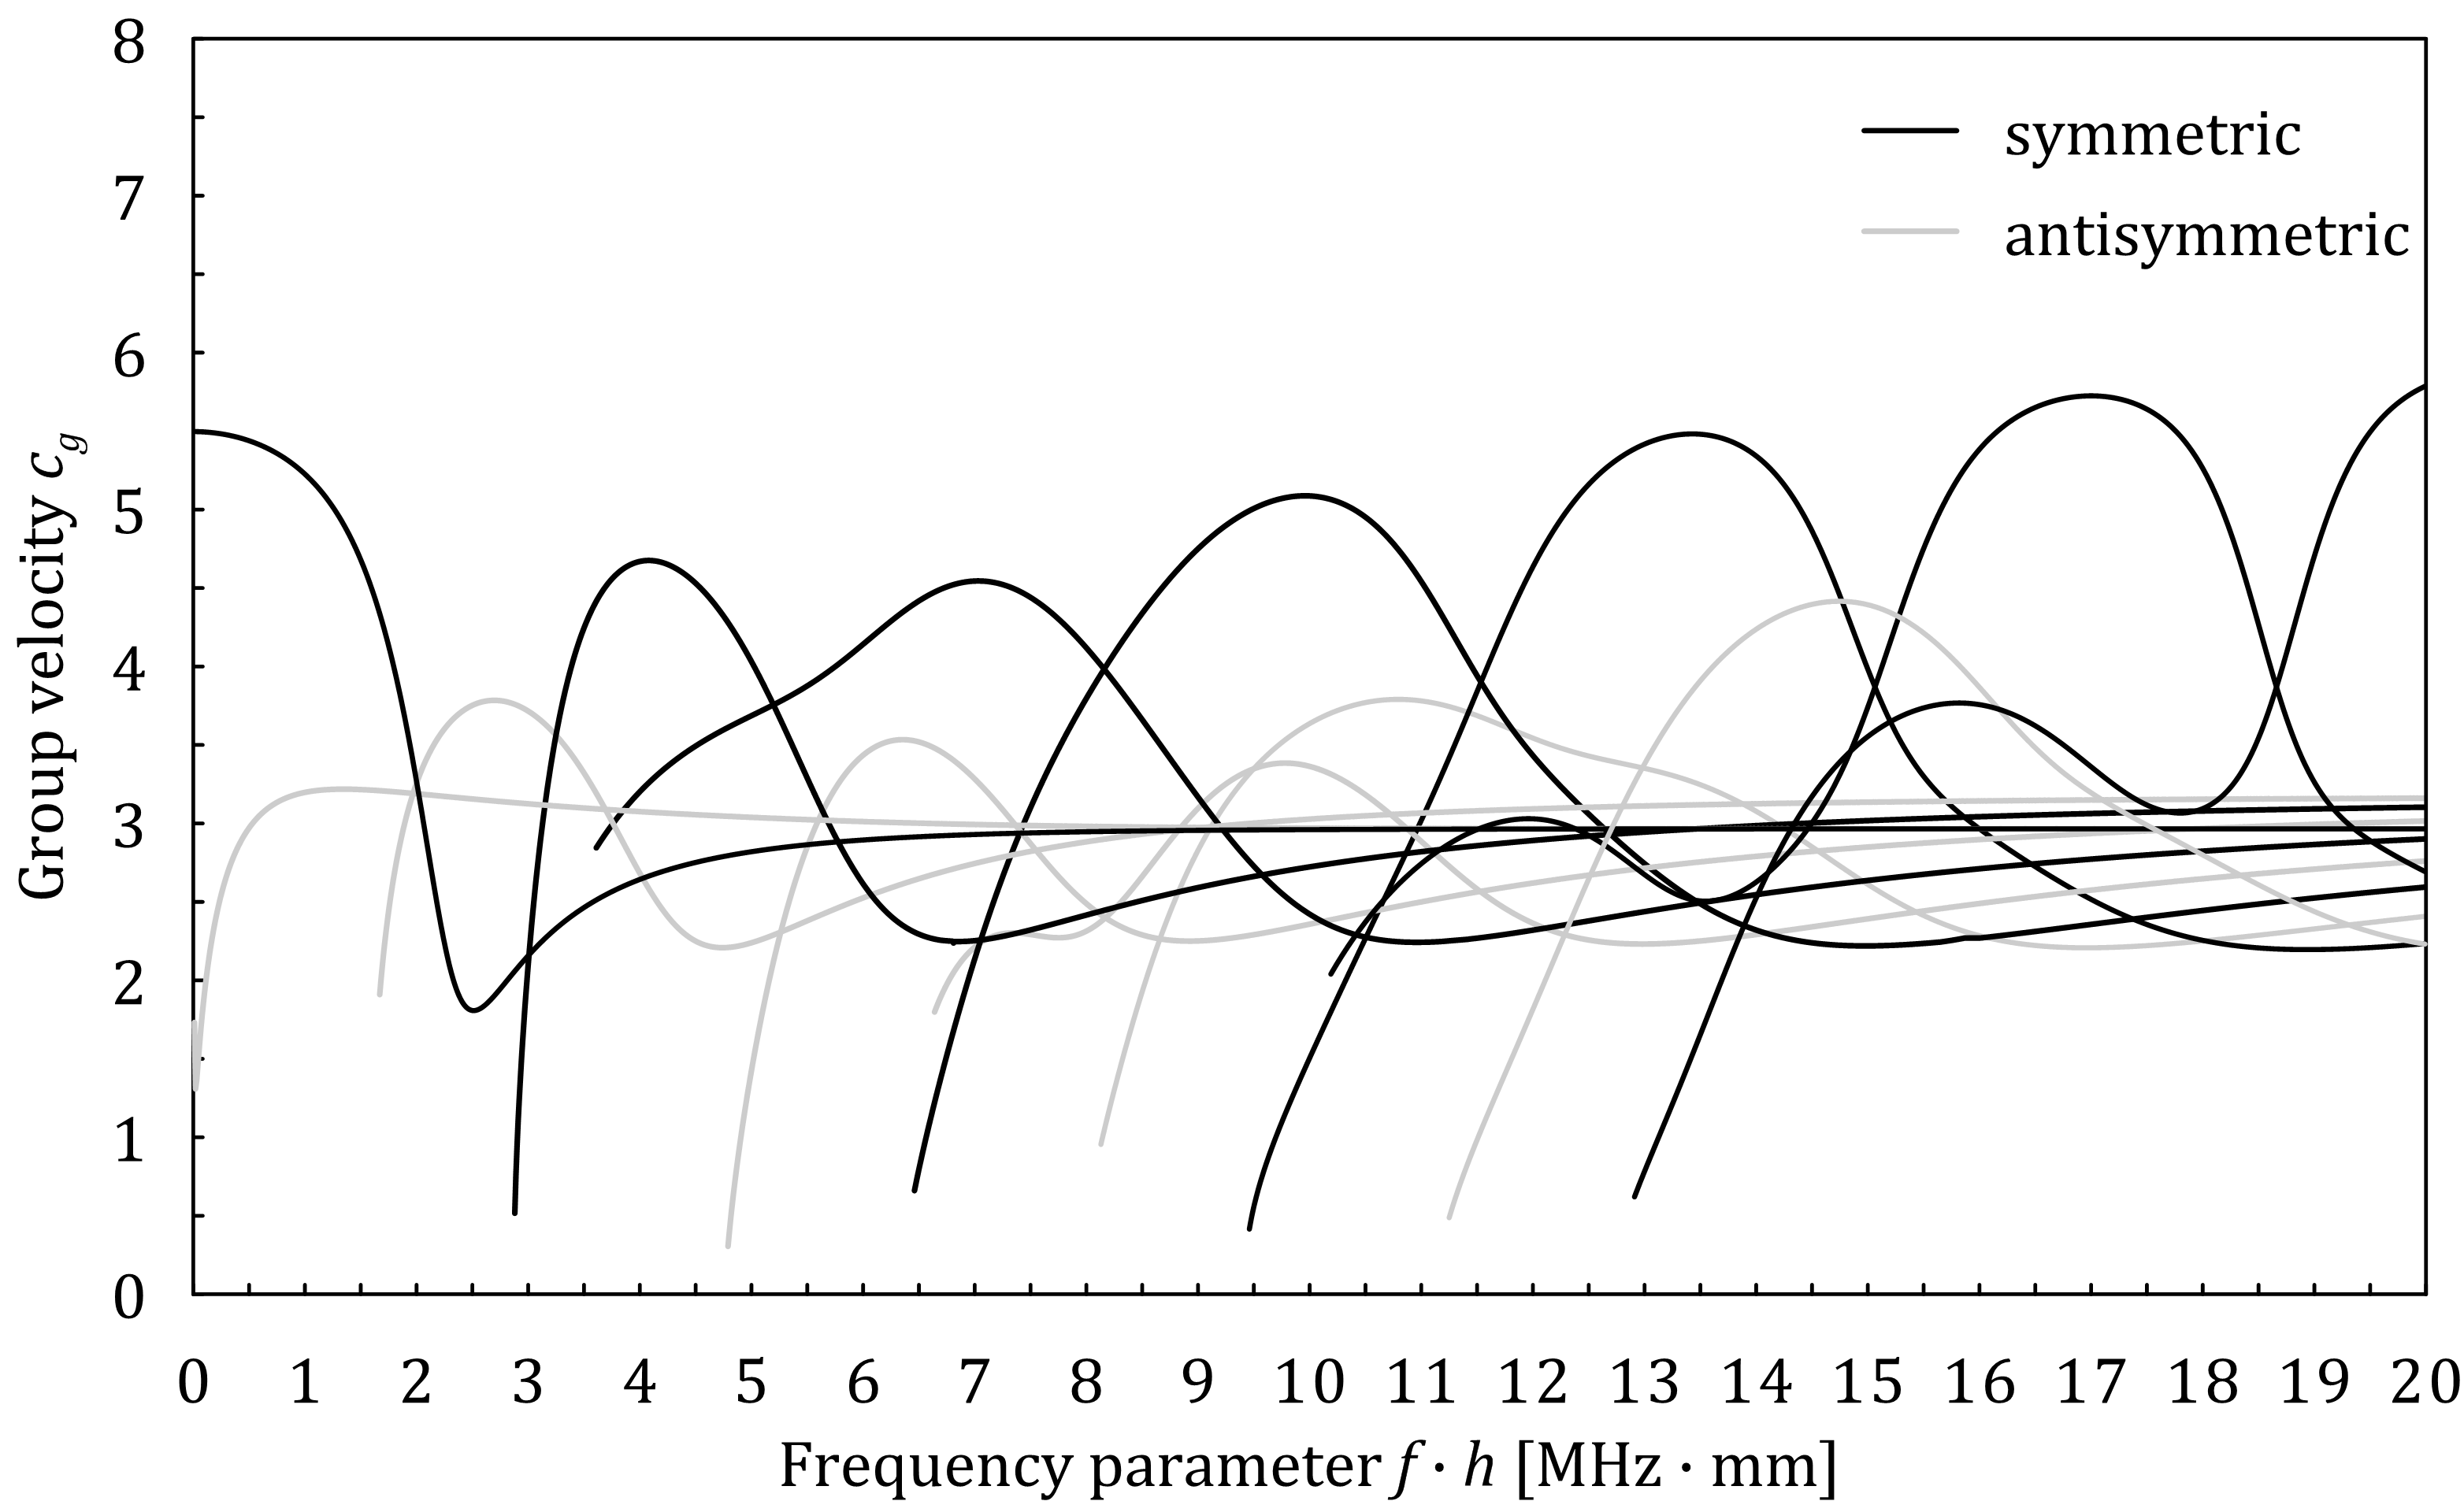
\includegraphics[width=0.8\textwidth]{/figs/Fig_1_13.png}	
%			}
%		\end{figure}
%	\end{frame}
	%%%%%%%%%%%%%%%%%%%%%%%%%%%%%%%%%%%%%%%%%%%%%%%%%%%%%%%%%%%%%%%%%%%%%%%%%%%%
	
	%%%%
	\setcounter{subfigure}{0}
	\section{Artificial intelligence, machine learning, and deep learning}
	%%%%%%%%%%%%%%%%%%%%%%%%%%%%%%%%%%%%%%%%%%%%%%%%%%
	%%%%%%%%%%%%%%%%%%%%%%%%%%%%%%%%%%%%%%%%%%%%%%%%%%
	\begin{frame}{What is AI?}
		\begin{figure}
				\centering
				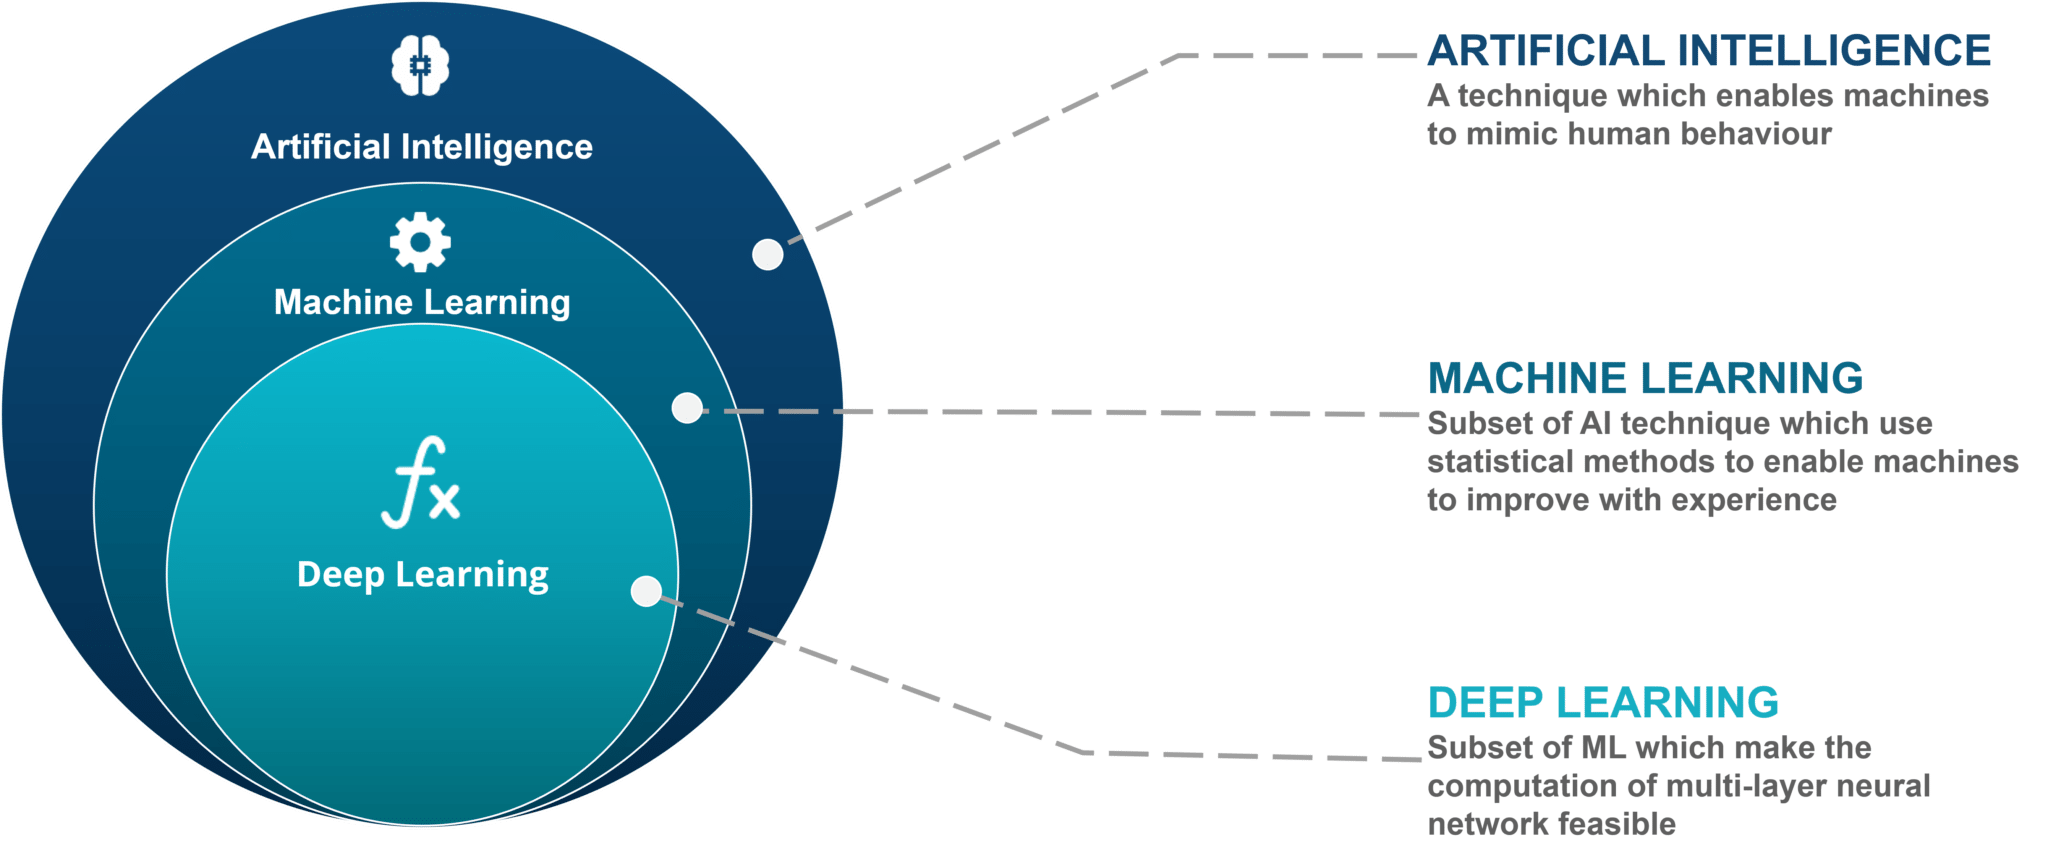
\includegraphics[width=0.85\textwidth]{AI_vs_ML_vs_Deep_Learning.png}
			\end{figure}
		\tiny
		(source: https://www.ingeniovirtual.com/)
	\end{frame}
	%%%%%%%%%%%%%%%%%%%%%%%%%%%%%%%%%%%%%%%%%%%%%%%%%%%%%%%%%%%%%%%%%%%%%%%%%%%%
	\note{
		Artificial intelligence (AI) refers to the development of computer systems or machines that can perform tasks that typically require human intelligence. It is a broad field of study and encompasses various subfields, including machine learning, natural language processing, computer vision, robotics, and more.
		
		AI systems aim to simulate and replicate human cognitive functions, such as perception, reasoning, learning, problem-solving, and decision-making. These systems can analyze and interpret complex data, recognize patterns, make predictions, understand natural language, and interact with humans and their environment.
		
		AI techniques can be categorized into two main types:
		
		Narrow AI: Also known as weak AI, narrow AI focuses on specific tasks and is designed to perform well in a limited domain. Examples of narrow AI include virtual personal assistants (such as Siri or Alexa), recommendation systems, image or speech recognition systems, and autonomous vehicles.
		
		General AI: General AI refers to highly autonomous systems that possess the ability to understand, learn, and perform any intellectual task that a human being can do. General AI aims to have a level of intelligence that is comparable to or surpasses human intelligence across various domains. However, the development of true general AI is still a subject of ongoing research and remains a future goal.
		
		AI has numerous applications across various industries, including healthcare, finance, transportation, education, manufacturing, and entertainment. It has the potential to revolutionize many aspects of our lives, driving advancements in automation, personalized services, data analysis, and decision support.}
	
	%%%%%%%%%%%%%%%%%%%%%%%%%%%%%%%%%%%%%%%%%%%%%%%%%%%%%%%%%%%%%%%%%%%%%%%%%%%%
	\setcounter{subfigure}{0}
	%%%%%%%%%%%%%%%%%%%%%%%%%%%%%%%%%%%%%%%%%%%%%%%%%%
	\begin{frame}{Why now?}
		\begin{columns}[T]
			\begin{column}[c]{0.4\textwidth}
				AI technologies are in accelerating growth due to:
				\begin{itemize}
					\item Exponential development in computer hardware industries
					(e.g. CPUs, GPUs, FPGAs, TPUs and ASICs)
					\item Era of Big data.
				\end{itemize}
			\end{column}
			\begin{column}[c]{0.55\textwidth}
				\begin{figure}
					\centering
					\subfloat{\animategraphics[autoplay,loop,width=.9\textwidth]{10}{gif_figs/gpu/gpu_-}{0}{34}}
				\end{figure}
				\tiny
				(source: https://www.techbooky.com/)
			\end{column}
		\end{columns}		
	\end{frame}
	%%%%%%%%%%%%%%%%%%%%%%%%%%%%%%%%%%%%%%%%%%%%%%%%%%%
	\setcounter{subfigure}{0}
	%%%%%%%%%%%%%%%%%%%%%%%%%%%%%%%%%%%%%%%%%%%%%%%%%%
	\begin{frame}{Common learning strategies}
		\centering
		\begin{figure}
			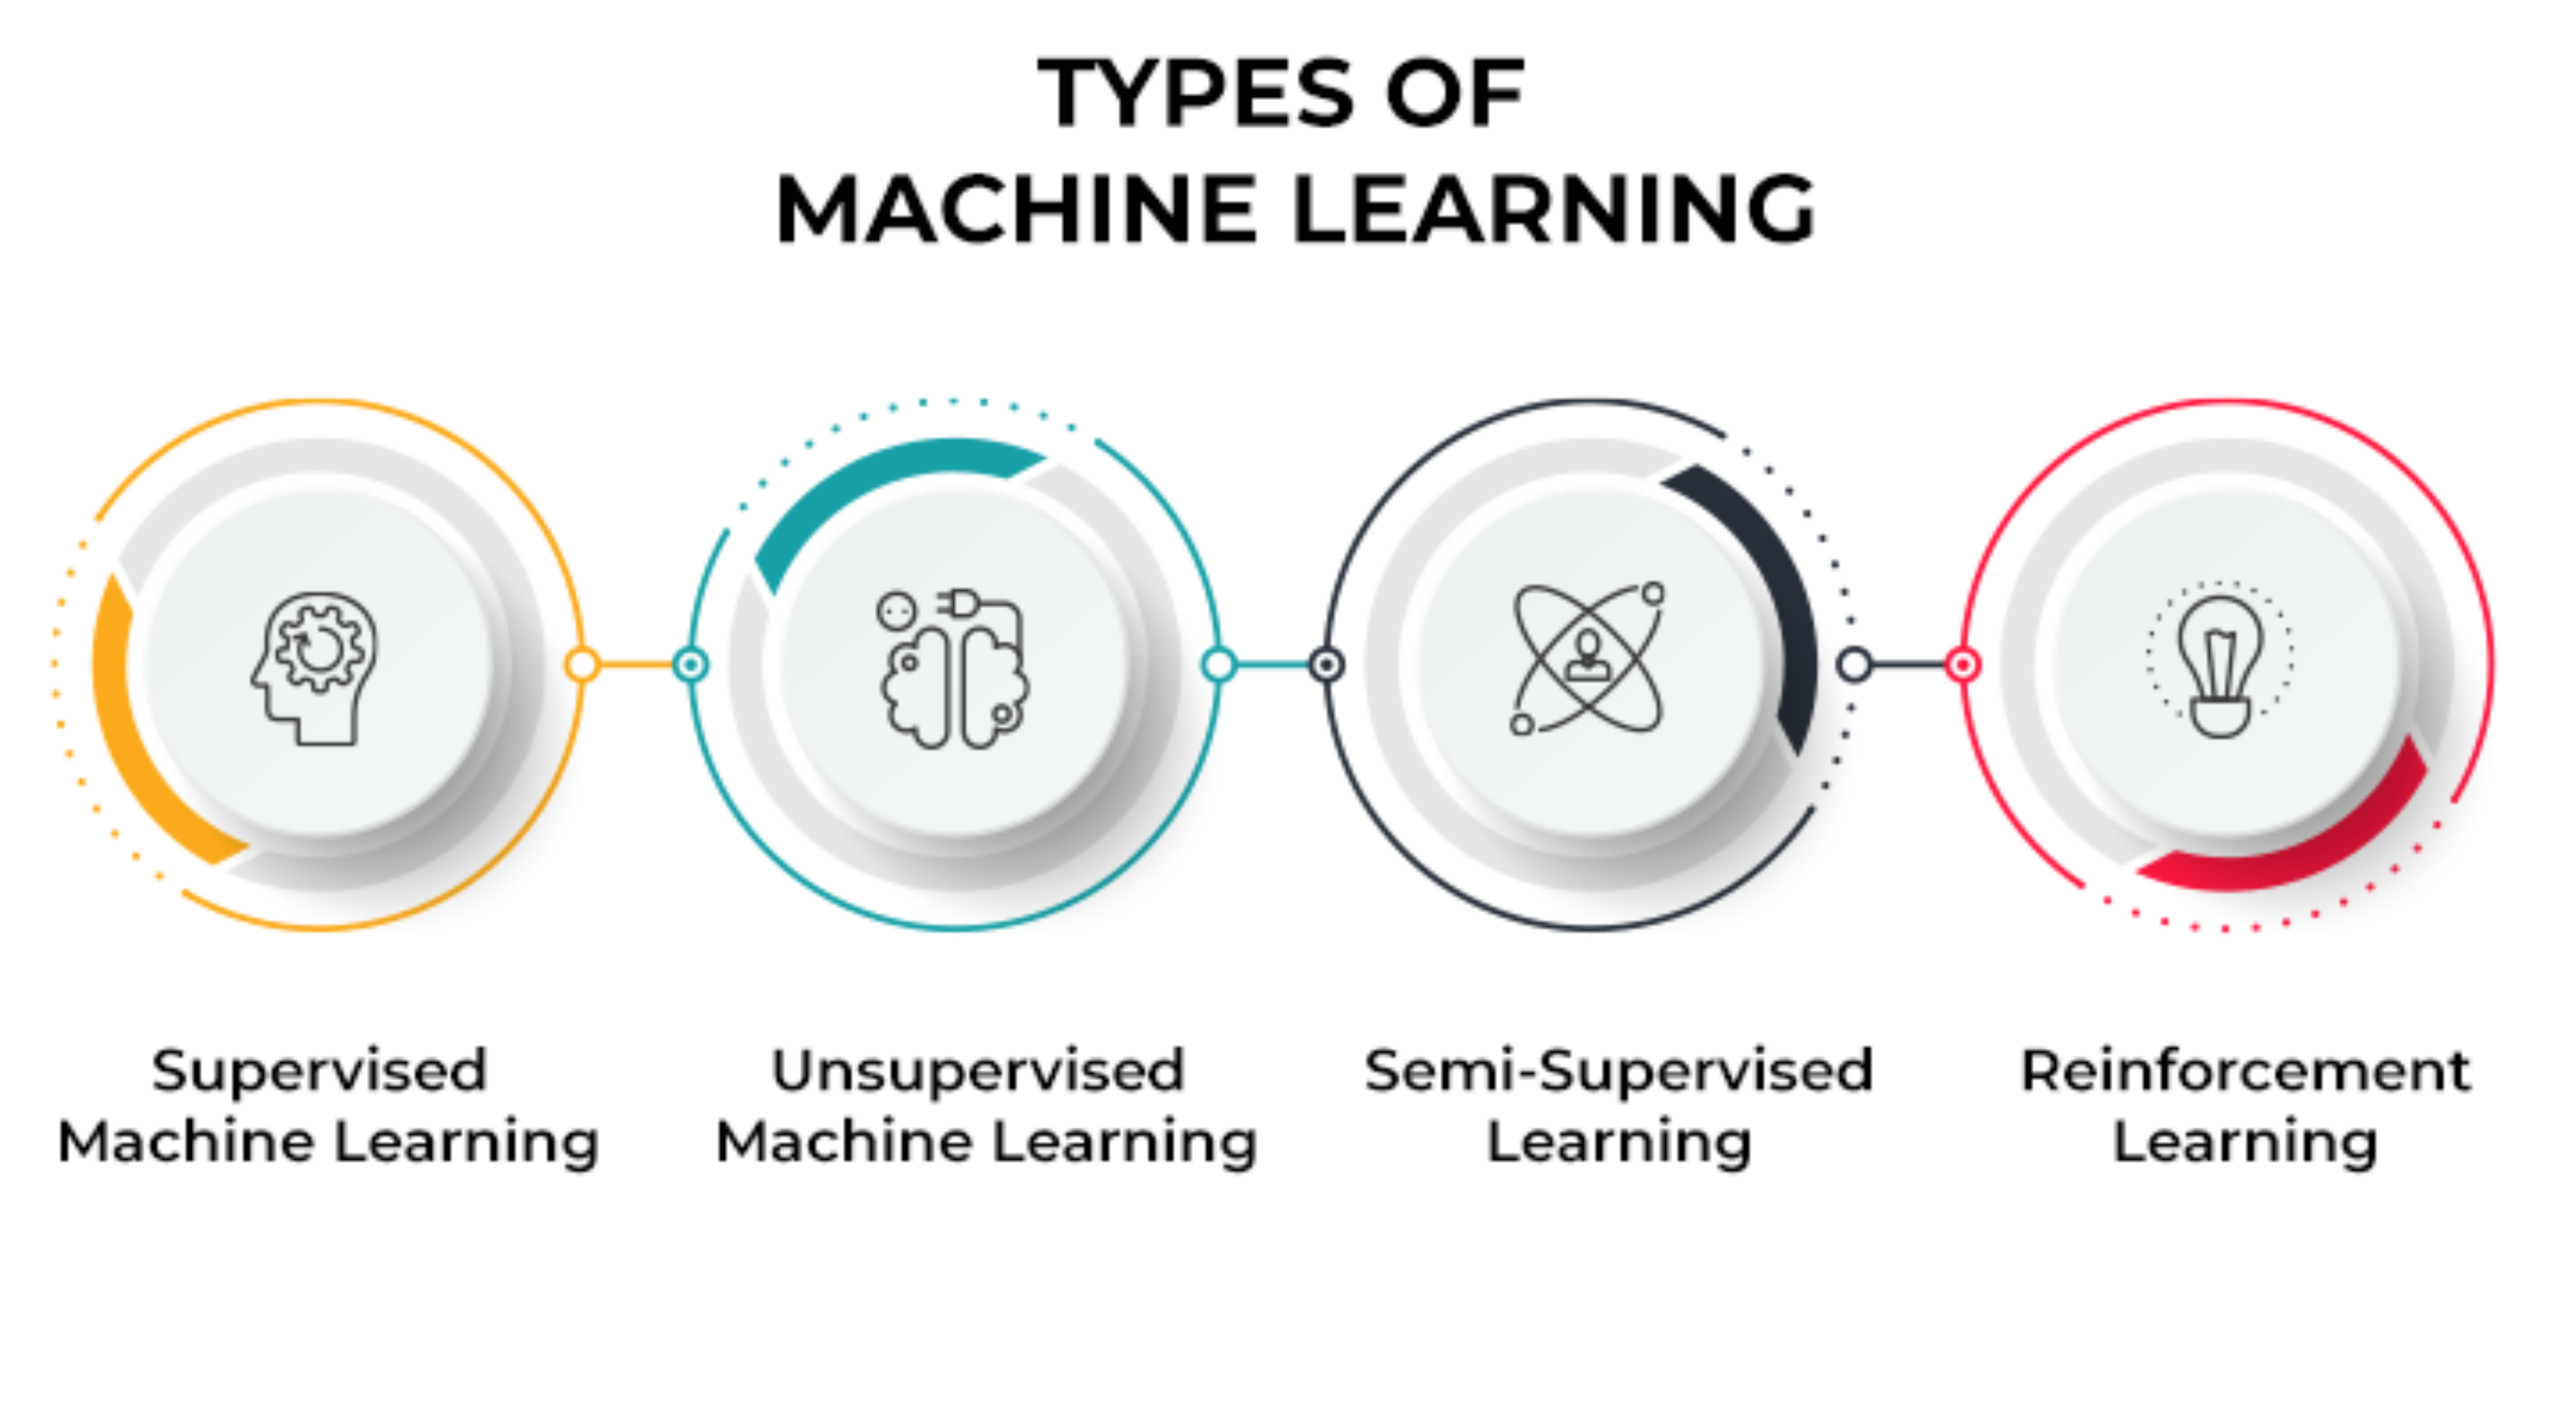
\includegraphics[width=0.9\textwidth]{learning.png}
		\end{figure}
	\end{frame}
	\note{
	In artificial intelligence, there are several common learning strategies or approaches used to train models and enable them to acquire knowledge from data. Here are some of the key learning strategies:
	
	Supervised Learning: In supervised learning, a model is trained on a labelled dataset where both input features and corresponding output labels are provided. The model learns to map inputs to outputs by minimizing the discrepancy between its predictions and the true labels. This approach is commonly used for tasks like classification and regression.
	
	Unsupervised Learning: Unsupervised learning involves training a model on an unlabelled dataset. The goal is to discover hidden patterns, structures, or relationships in the data without any predefined output labels. Clustering, dimensionality reduction, and anomaly detection are examples of unsupervised learning tasks.
	
	Semi-Supervised Learning: Semi-supervised learning combines labelled and unlabelled data to train a model. It leverages the small amount of labeled data along with the larger pool of unlabelled data to improve performance. This approach is useful when obtaining labelled data is expensive or time-consuming.
		
	Reinforcement Learning: Reinforcement learning involves training an agent to interact with an environment and learn optimal actions based on feedback in the form of rewards or punishments. The agent learns through trial and error to maximize cumulative rewards, discovering a policy that guides its decision-making. Reinforcement learning is often used in scenarios such as game playing, robotics, and control systems.
	
	Transfer Learning: Transfer learning involves training a model on one task and then applying the learned knowledge to a different but related task. The idea is to transfer the learned representations or knowledge from the source task to the target task, which can help in cases where the target task has limited labelled data available.
	
	Generative Modeling: Generative models aim to learn the underlying probability distribution of the data in order to generate new samples that are similar to the training data. Examples include generative adversarial networks (GANs) and variational autoencoders (VAEs). Generative models have applications in image synthesis, text generation, and data augmentation.
	
	These are some of the common learning strategies in artificial intelligence. Different approaches are suitable for different problem domains, and often a combination of these strategies is used to tackle complex tasks or real-world scenarios.
	}
	%%%%%%%%%%%%%%%%%%%%%%%%%%%%%%%%%%%%%%%%%%%%%%%%%%%%%%%%%%%%%%%%%%%%%%%%%%%%
	\section{AI approaches for Anomaly detection}
	%%%%%%%%%%%%%%%%%%%%%%%%%%%%%%%%%%%%%%%%%%%%%%%%%%%%%%%%%%%%%%%%%%%%%%%%%%%%
	\begin{frame}{Machine learning approach}
		Machine learning techniques involve two processes:
		\alert{\textbf{Feature extraction and classification}}
		\begin{itemize}
			\item \alert{\textbf{Feature extraction}} \(\rightarrow\) includes signals preprocessing (signal denoising and averaging), then extracting \textbf{damage indexes (DIs)}.
			\item \alert{\textbf{Feature classification}}\(\rightarrow\) the extracted features are classified, for instance, into healthy or damaged states.
		\end{itemize}
		\begin{figure}
			\centering
			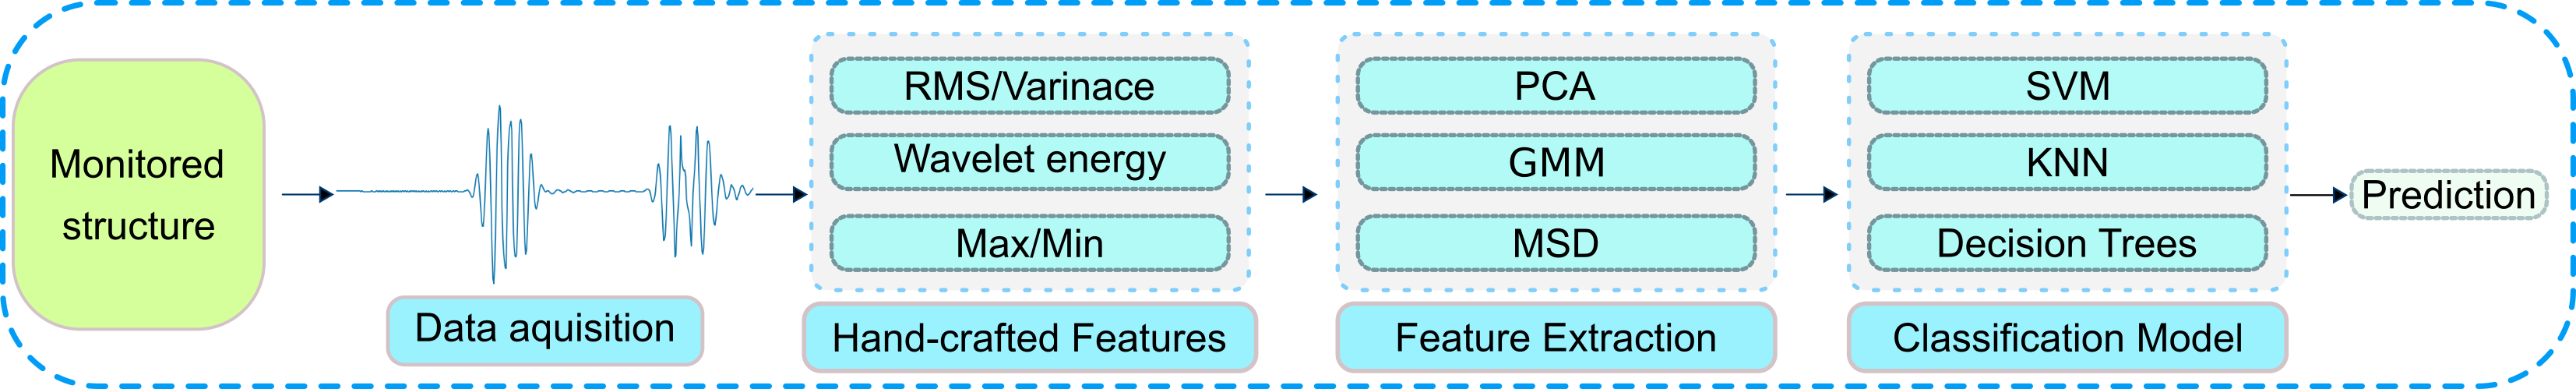
\includegraphics[width=.95\textwidth]{conventional_ML.png}
		\end{figure}
	\end{frame}
	\note{
		Feature extraction is a crucial step in machine learning and pattern recognition tasks. It involves transforming raw data into a representative set of features that capture relevant information for the given problem. Here are some commonly used techniques for feature extraction:
		
		Statistical Features: Statistical measures such as mean, median, standard deviation, skewness, and kurtosis can capture important characteristics of the data distribution.
		
		Fourier Transform: The Fourier transform decomposes a signal into its frequency components, revealing the presence of periodic patterns or oscillations in the data. Frequency domain features like power spectral density or dominant frequencies can be extracted.
		
		Wavelet Transform: The wavelet transform represents signals at multiple scales, capturing both time and frequency information. Wavelet-based features are useful for analyzing transient or non-stationary signals.
		
		Principal Component Analysis (PCA): PCA is a dimensionality reduction technique that identifies the most important orthogonal directions (principal components) in the data. It helps to capture the maximum variance and reduce the dimensionality of the feature space.
		
		Independent Component Analysis (ICA): ICA aims to separate a multivariate signal into additive subcomponents, assuming they are statistically independent. ICA is useful for separating mixed signals or sources from a set of observations.
		
		Mel-Frequency Cepstral Coefficients (MFCC): MFCC is commonly used for audio signal processing. It involves transforming the audio spectrum using the mel scale and extracting cepstral coefficients that represent the spectral envelope of the signal.
		
		Image-based Features: In computer vision, features such as edge detection, texture descriptors (e.g., Local Binary Patterns), color histograms are commonly used to represent images.
	
		The choice of feature extraction technique depends on the nature of the data, the problem at hand, and the available domain knowledge. It often requires experimentation and domain expertise to identify the most informative set of features for a given task.
		
		Feature classification, also known as feature learning or pattern recognition, is the process of assigning or labeling data samples into predefined classes or categories based on the extracted features. It is a fundamental task in machine learning and is often used for tasks such as object recognition, image classification, text categorization, and speech recognition. Various techniques can be employed for feature classification, including:
		
		Supervised Learning: In supervised learning, labeled training data is used to train a classification model that can map input features to their corresponding class labels. Some commonly used supervised learning algorithms include:
		
		Decision Trees
		Random Forests
		Support Vector Machines (SVM)
		Naive Bayes
		k-Nearest Neighbors (k-NN)
		Logistic Regression
		Neural Networks (e.g., Multi-layer Perceptron)
		Unsupervised Learning: Unsupervised learning does not rely on labeled data and aims to identify patterns or groupings in the data without explicit class labels. Clustering algorithms are commonly used for unsupervised feature classification:
		
		K-means Clustering
		Hierarchical Clustering
		DBSCAN (Density-Based Spatial Clustering of Applications with Noise)
		Gaussian Mixture Models (GMM)
		Ensemble Methods: Ensemble methods combine multiple classifiers to improve the overall classification performance. Popular ensemble techniques include:
		
		Bagging (Bootstrap Aggregating)
		Boosting (e.g., AdaBoost, Gradient Boosting)
		Random Forests
		Deep Learning: Deep learning approaches, particularly deep neural networks, have gained significant popularity in recent years for feature classification tasks. Deep neural networks can learn complex feature representations directly from raw data, leading to state-of-the-art performance in various domains. Some commonly used deep learning architectures for classification include:
		
		Convolutional Neural Networks (CNN)
		Recurrent Neural Networks (RNN)
		Long Short-Term Memory (LSTM) Networks
		Transformer Networks
		Dimensionality Reduction: Dimensionality reduction techniques can be used as a preprocessing step to reduce the number of features while retaining the most informative ones. Techniques like Principal Component Analysis (PCA) and t-SNE (t-Distributed Stochastic Neighbor Embedding) can help improve classification performance by reducing the feature space.
		
		Transfer Learning: Transfer learning leverages pre-trained models trained on large-scale datasets and fine-tunes them on a specific classification task with limited data. This approach is particularly useful when labeled data is scarce. Pre-trained models like VGG, ResNet, and BERT are often used in transfer learning.
		
		The choice of classification technique depends on various factors, including the nature of the data, the number of classes, the availability of labeled data, the desired computational efficiency, and the desired interpretability of the model. It often requires experimentation and tuning to determine the most suitable technique for a given classification task.
	}
	\begin{frame}{Drawbacks of Conventional methods}
		Conventional machine learning methods have several drawbacks, including:
		\begin{itemize}
			\item Feature Engineering
			\item Limited Ability to Handle High-Dimensional Data
			\item Lack of Scalability
			\item Lack of Adaptability to Changing Data
			\item Limited Representation Learning
			\item Interpretability	
		\end{itemize}
	\end{frame}

	%%%%%%%%%%%%%%%%%%%%%%%%%%%%%%%%%%%%%%%%%%%%%%%%%%%%%%%%%%%%%%%%%%%%%%%%%%%%
	\note{
		Conventional machine learning methods have several drawbacks, including:
		
		Feature Engineering: Conventional machine learning often requires manual feature engineering, where domain experts have to identify and select relevant features from the raw data. This process can be time-consuming, subjective, and may not always capture the full complexity of the data.
		
		Limited Ability to Handle High-Dimensional Data: Conventional methods can struggle when faced with high-dimensional data, such as images or text. The curse of dimensionality can lead to increased computational complexity and overfitting.
		
		Lack of Scalability: Some conventional machine learning algorithms, such as Support Vector Machines (SVMs), have computational complexity that scales poorly with large datasets. Training these models on massive datasets can become prohibitively time-consuming and resource-intensive.
		
		Manual Hyperparameter Tuning: Many conventional algorithms require careful tuning of hyperparameters, such as learning rates or regularization parameters, to achieve optimal performance. This process often relies on trial and error or expert knowledge, which can be labor-intensive and may not guarantee the best results.
		
		Lack of Adaptability to Changing Data: Conventional models are often trained on fixed datasets and may not easily adapt to changes in the underlying data distribution. This can make them less suitable for applications where the data distribution evolves over time, such as in online learning or real-time data streams.
		
		Limited Representation Learning: Traditional machine learning algorithms often struggle to automatically learn meaningful representations from raw data. They heavily rely on handcrafted features, which can be suboptimal or fail to capture the intricacies of complex patterns in the data.
		
		Interpretability: While interpretability is not always a drawback, some conventional methods, such as deep neural networks, can be difficult to interpret. Understanding the inner workings of these models and explaining their decisions to stakeholders can be challenging, limiting their usability in certain domains.
		
		It's important to note that while conventional machine learning methods have their limitations, they have been successfully applied in numerous domains and continue to be valuable in many practical applications. However, newer approaches, such as deep learning and other advancements in artificial intelligence, have emerged to address some of these drawbacks and push the boundaries of what is achievable with machine learning.
	
	}
	%%%%%%%%%%%%%%%%%%%%%%%%%%%%%%%%%%%%%%%%%%%%%%%%%%%%%%%%%%%%%%%%%%%%%%%%%%%%
	\setcounter{subfigure}{0}
	%%%%%%%%%%%%%%%%%%%%%%%%%%%%%%%%%%%%%%%%%%%%%%%%%%%%%%%%%%%%%%%%%%%%%%%%%%%	
	\begin{frame}{Deep learning approach}
		\textbf{Deep learning (DL) technologies are in accelerating growth due to:}
		\begin{itemize}
			\item \textcolor{blue}{Exponential development in computer hardware/software industries.}
			\item \textcolor{blue}{Machine learning algorithms.}
			\item \textcolor{blue}{Era of Big data.}
		\end{itemize}	
		Deep learning offers an \alert{\textbf{end-to-end}} approach: \alert{\textbf{Automatic}} feature extraction and classification.
		\begin{figure}
			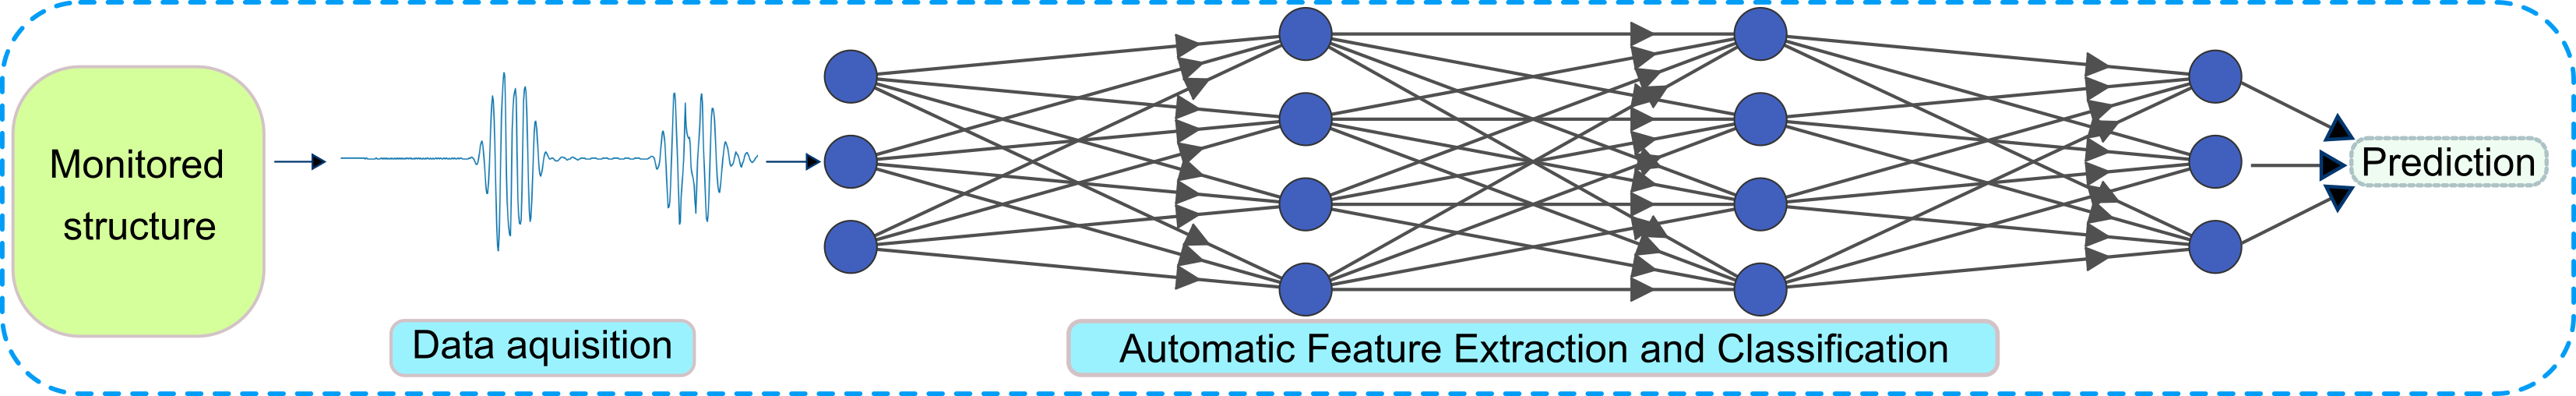
\includegraphics[width=.95\textwidth]{DL_approach.png}
		\end{figure}
	\end{frame}
	%%%%%%%%%%%%%%%%%%%%%%%%%%%%%%%%%%%%%%%%%%%%%%%%%%
	\begin{frame}{Artificial neural networks (ANNs)}
		\begin{columns}[T]
			\begin{column}{.45\textwidth}
				\begin{block}{Artificial neuron}
					\begin{figure}
						\centering
						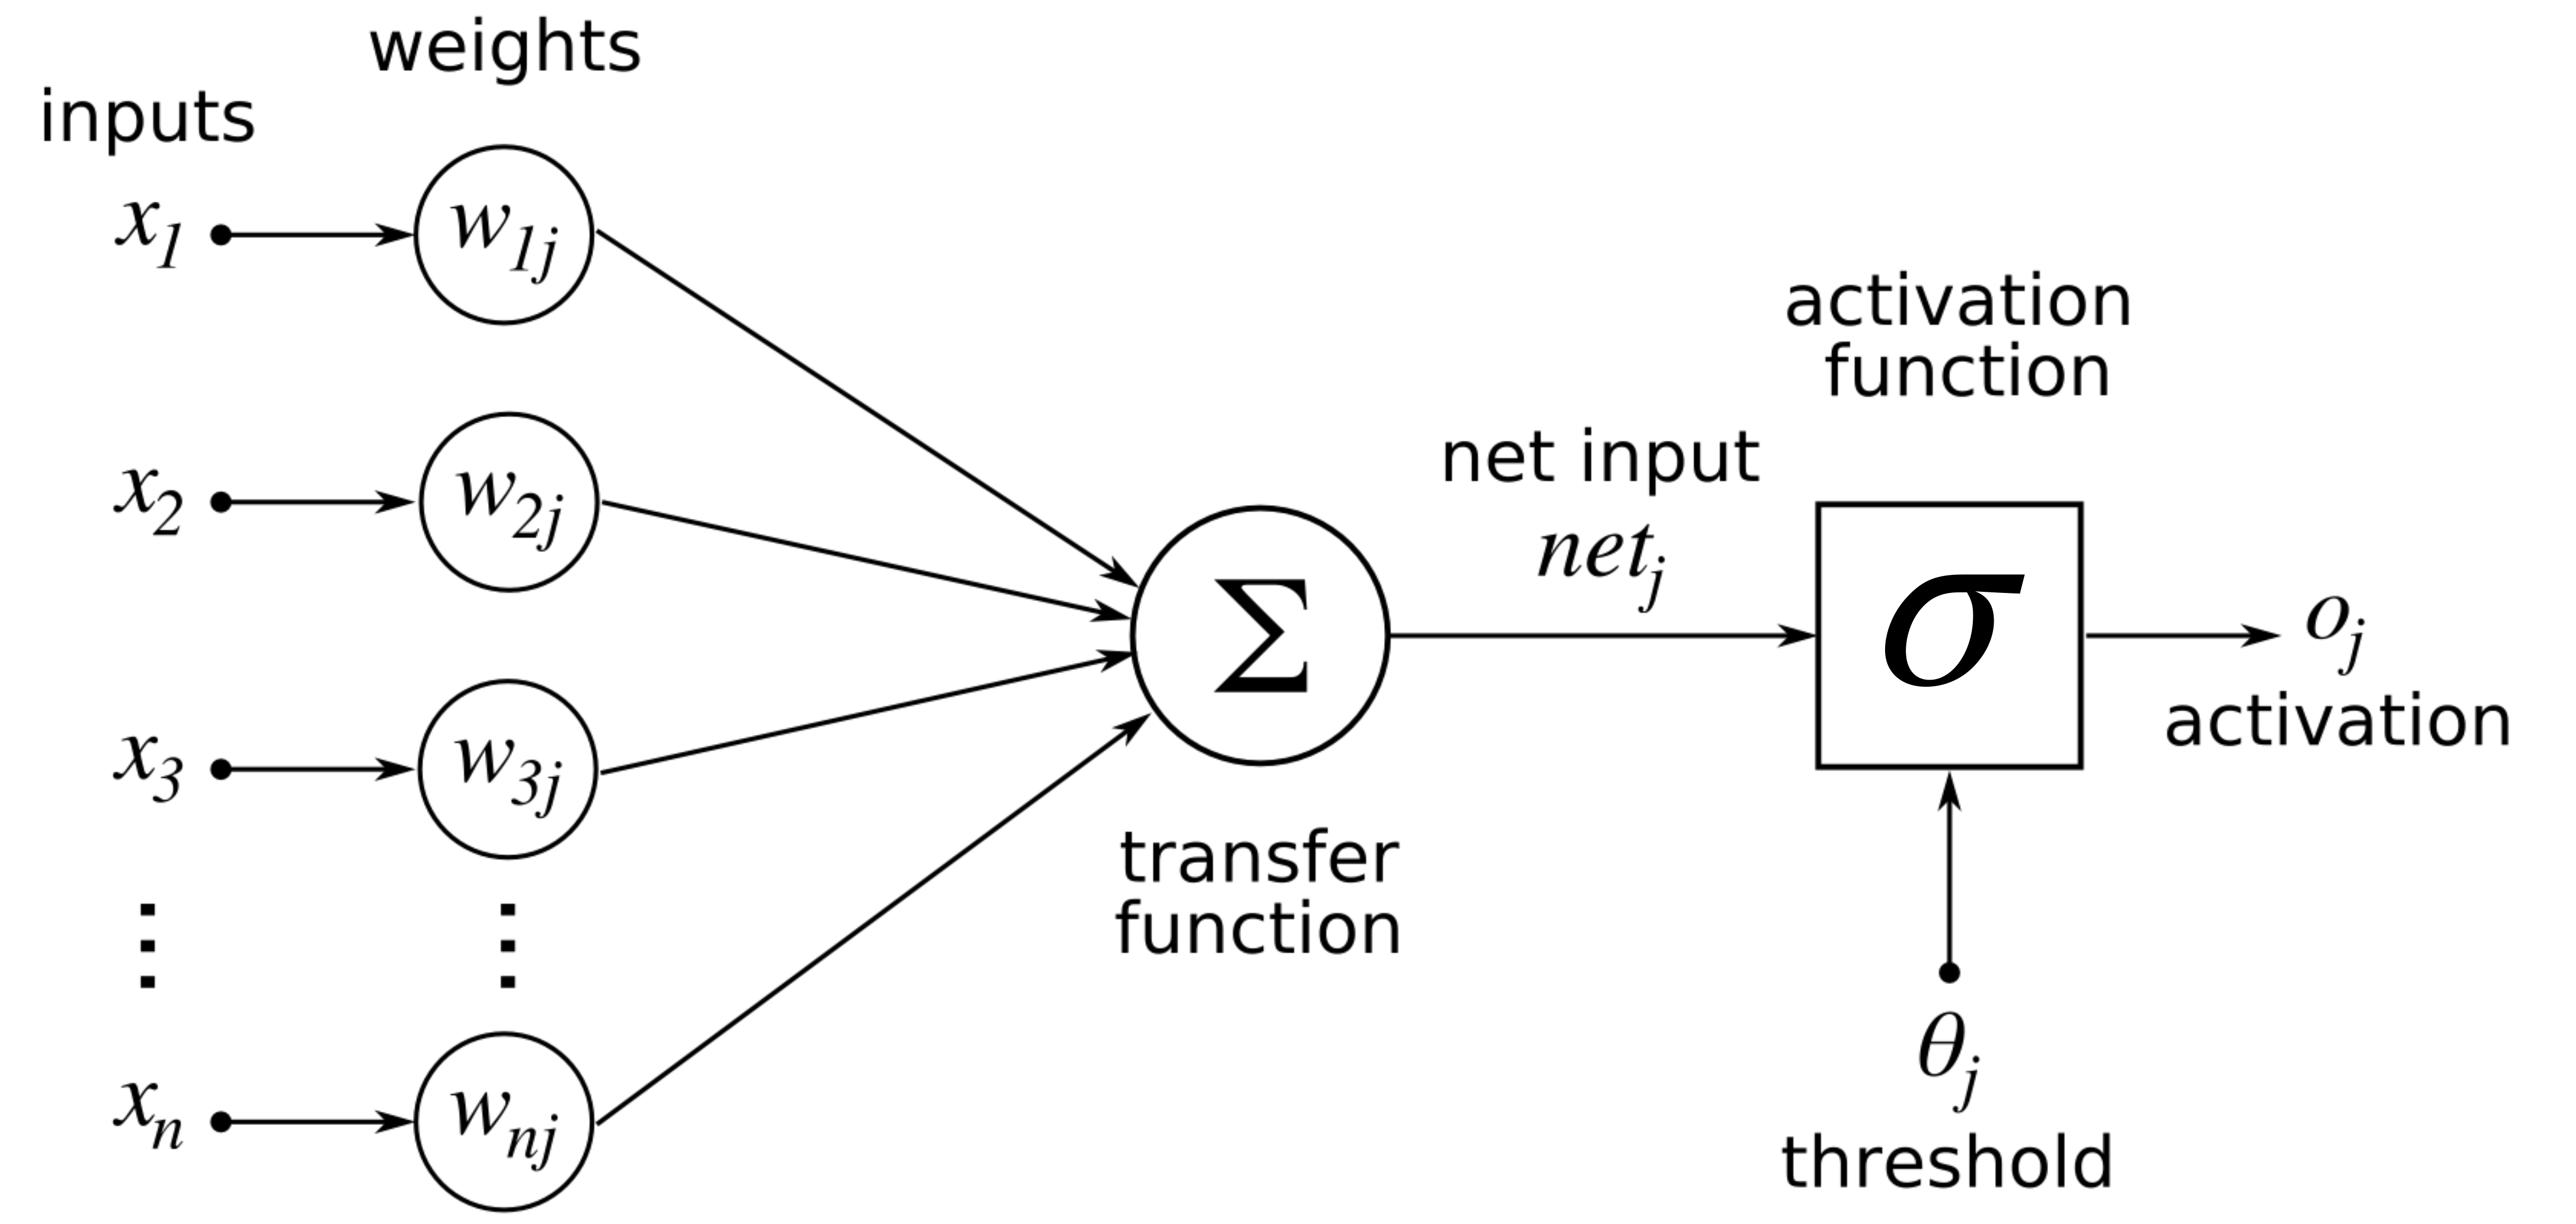
\includegraphics[width=.95\textwidth]{ArtificialNeuronModel.png}
					\end{figure}
				The equation for an artificial neuron is given by:
				\[
				y = \sigma\left(\sum_{i=1}^{n} w_i x_i + b\right)
				\]
				\end{block}
			\end{column}
			\begin{column}{0.55\textwidth}
				\begin{block}{ANN}
					\begin{figure}
						\centering
						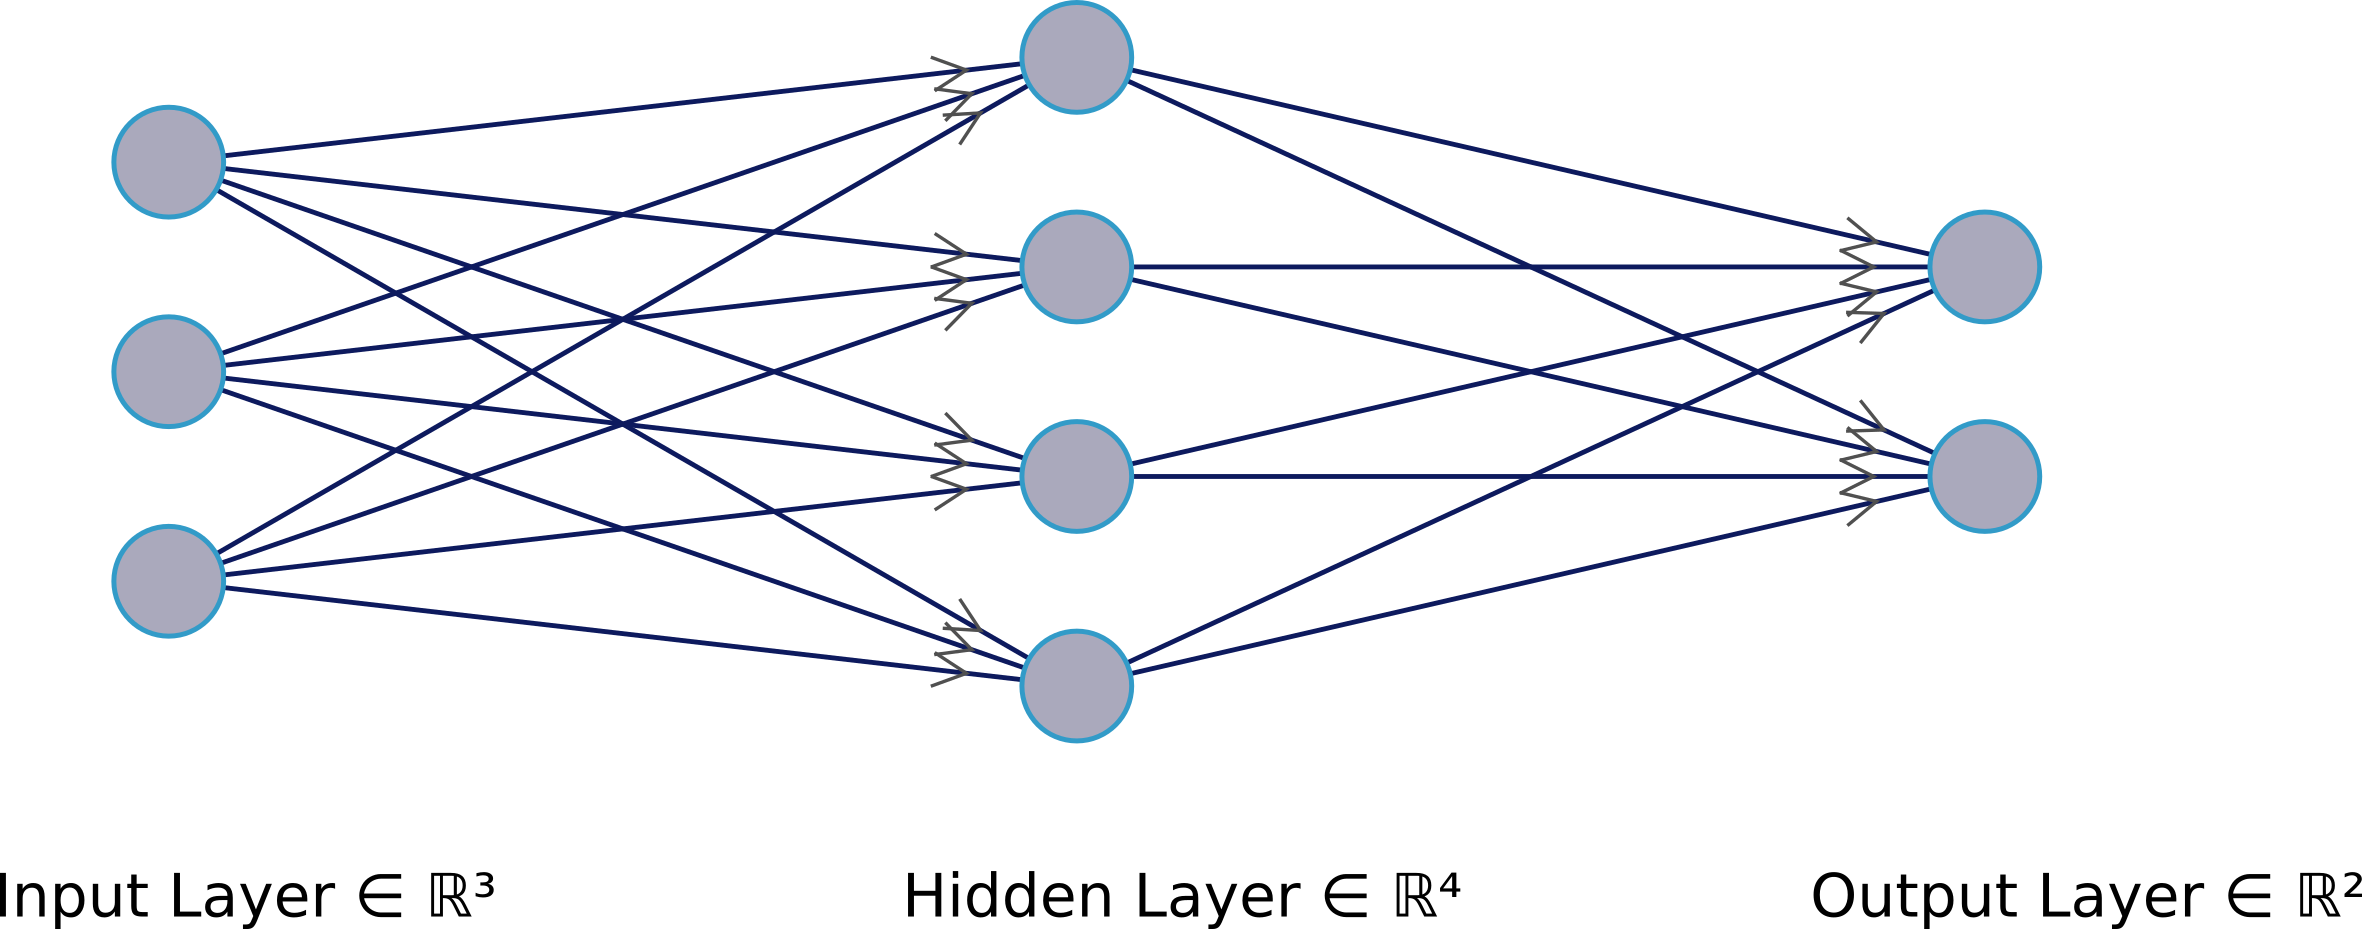
\includegraphics[width=0.85\textwidth]{ANN.png}
					\end{figure}
					ANN can be created by cascading n-layers of “neurons”. 
					\begin{itemize}
						\item	Input layer.
						\item	Hidden layer(s).
						\item	Output layer.	
					\end{itemize}
				\end{block}
			\end{column}
		\end{columns}
	\end{frame}
	\setcounter{subfigure}{0}
	\begin{frame}{Optimization and Deep Learning}
		\begin{columns}[T]
			\begin{column}[t]{.4\textwidth}
				\begin{itemize}
					\item \alert{Labelled data} $\rightarrow$ (input data has labels/ground truths)
					\item \alert{Loss function} $\rightarrow$ measures error between predicted and the ground truth values
					\item \alert{Learnable parameters} $\rightarrow$ updated during the backpropagation step (optimization e.g. Gradient descent )					
				\end{itemize}
			\end{column}
			\begin{column}[t]{.55\textwidth}
				\begin{figure}[t]
					\centering
					\animategraphics[autoplay,loop,width =1.0\textwidth]{1}{figures/gif_figs/BP/png/BP_technique_}{0}{14}
				\end{figure}
			\end{column}
		\end{columns}		
	\end{frame}
	%%%%%%%%%%%%%%%%%%%%%%%%%%%%%%%%%%%%%%%%%%%%%%%%%%%%%%%%%%%%%%%%%%%%%%%%%%%%
	\note{			
		In this work, I used the supervised approach, which means that the input data is labelled.
		
		Accordingly, the idea of supervised learning is to learn a model of how to map the inputs to the outputs.
		
		Initially, when we start training the deep learning model, all learnable parameters, such as weights and biases, start with random values.
		These learnable parameters are updated during the training phase.
		Now, in the forward pass, we feed the data into the model, and it flows through the layers until we get the predicted output.
		Here, we need an objective loss function to estimate the loss (error) between the predicted output and the ground truth.
		
		A well-known optimization algorithm is a gradient descent, which aims to reduce the loss at each step to reach the global minimum value by calculating the gradient and then pushing back the calculated gradients across all the neurons in a technique called backpropagation.
		
		Accordingly, all learnable parameters are updated, which leads to minimizing the loss value.
	}
	
	%%%%%%%%%%%%%%%%%%%%%%%%%%%%%%%%%%%%%%%%%%%%%%%%%%%%%%%%%%%%%%%%%%%%%%%%%%%%
	\begin{frame}{Convolution Neural Networks (CNNs)}
		\noindent Convolutional Neural Network (CNN) is one of the most utilised architectures in DL for image processing as they can \alert{recognise complex patterns} of images by performing \alert{convolution operations}.
		
		Convolution in DL is a cross-correlation operation \alert{(sliding dot product)}. \\
		The kernel weights \alert{(learnable weights)} are updated during training phase.
		\begin{figure}[t]
			\centering
			\animategraphics[autoplay,loop,width =1.0\textwidth]{1}{figures/gif_figs/files/plot_convolution_process_}{0}{32}
		\end{figure}
	\end{frame}
	%%%%%%%%%%%%%%%%%%%%%%%%%%%%%%%%%%%%%%%%%%%%%%%%%%%%%%%%%%%%%%%%%%%%%%%%%%%%
	\note{
		Convolutional Neural Network (CNN) is a powerful deep learning architecture for image processing because it can extract complex feature patterns from images using convolution operations.
		
		The convolution operation for image processing is essentially a cross-correlation operation, also known as a sliding dot product or sliding inner product.
		
		The kernel slides over an input image of performing a convolution operation.
		The output of the convolution operation is a feature map.
		
		Consequently, kernels learn to detect different types of edges
		(vertical, horizontal, and diagonal edges), colour intensities, etc.	
		
		%		Typically, when we train a CNN model, the kernel weights are initialised randomly.
		
		During the backpropagation process, all kernel weights are updated. 				
	}
	%%%%%%%%%%%%%%%%%%%%%%%%%%%%%%%%%%%%%%%%%%%%%%%%%%%%%%%%%%%%%%%%%%%%%%%%%%%%
	\setcounter{subfigure}{0}
	\begin{frame}{Encoder-decoder (Autoencoder)}
		\begin{columns}[T]
			\begin{column}[t]{.35\textwidth}
				\begin{itemize}
					\item \alert{Encoder} learns to extract features.
					\item \alert{Latent space} has condensed feature maps.
					\item \alert{Decoder} learns to locate the features learned by the encoder.
				\end{itemize}	
			\end{column}
			\hfill
			\begin{column}[t]{.6\textwidth}
				\begin{figure}
					\centering
					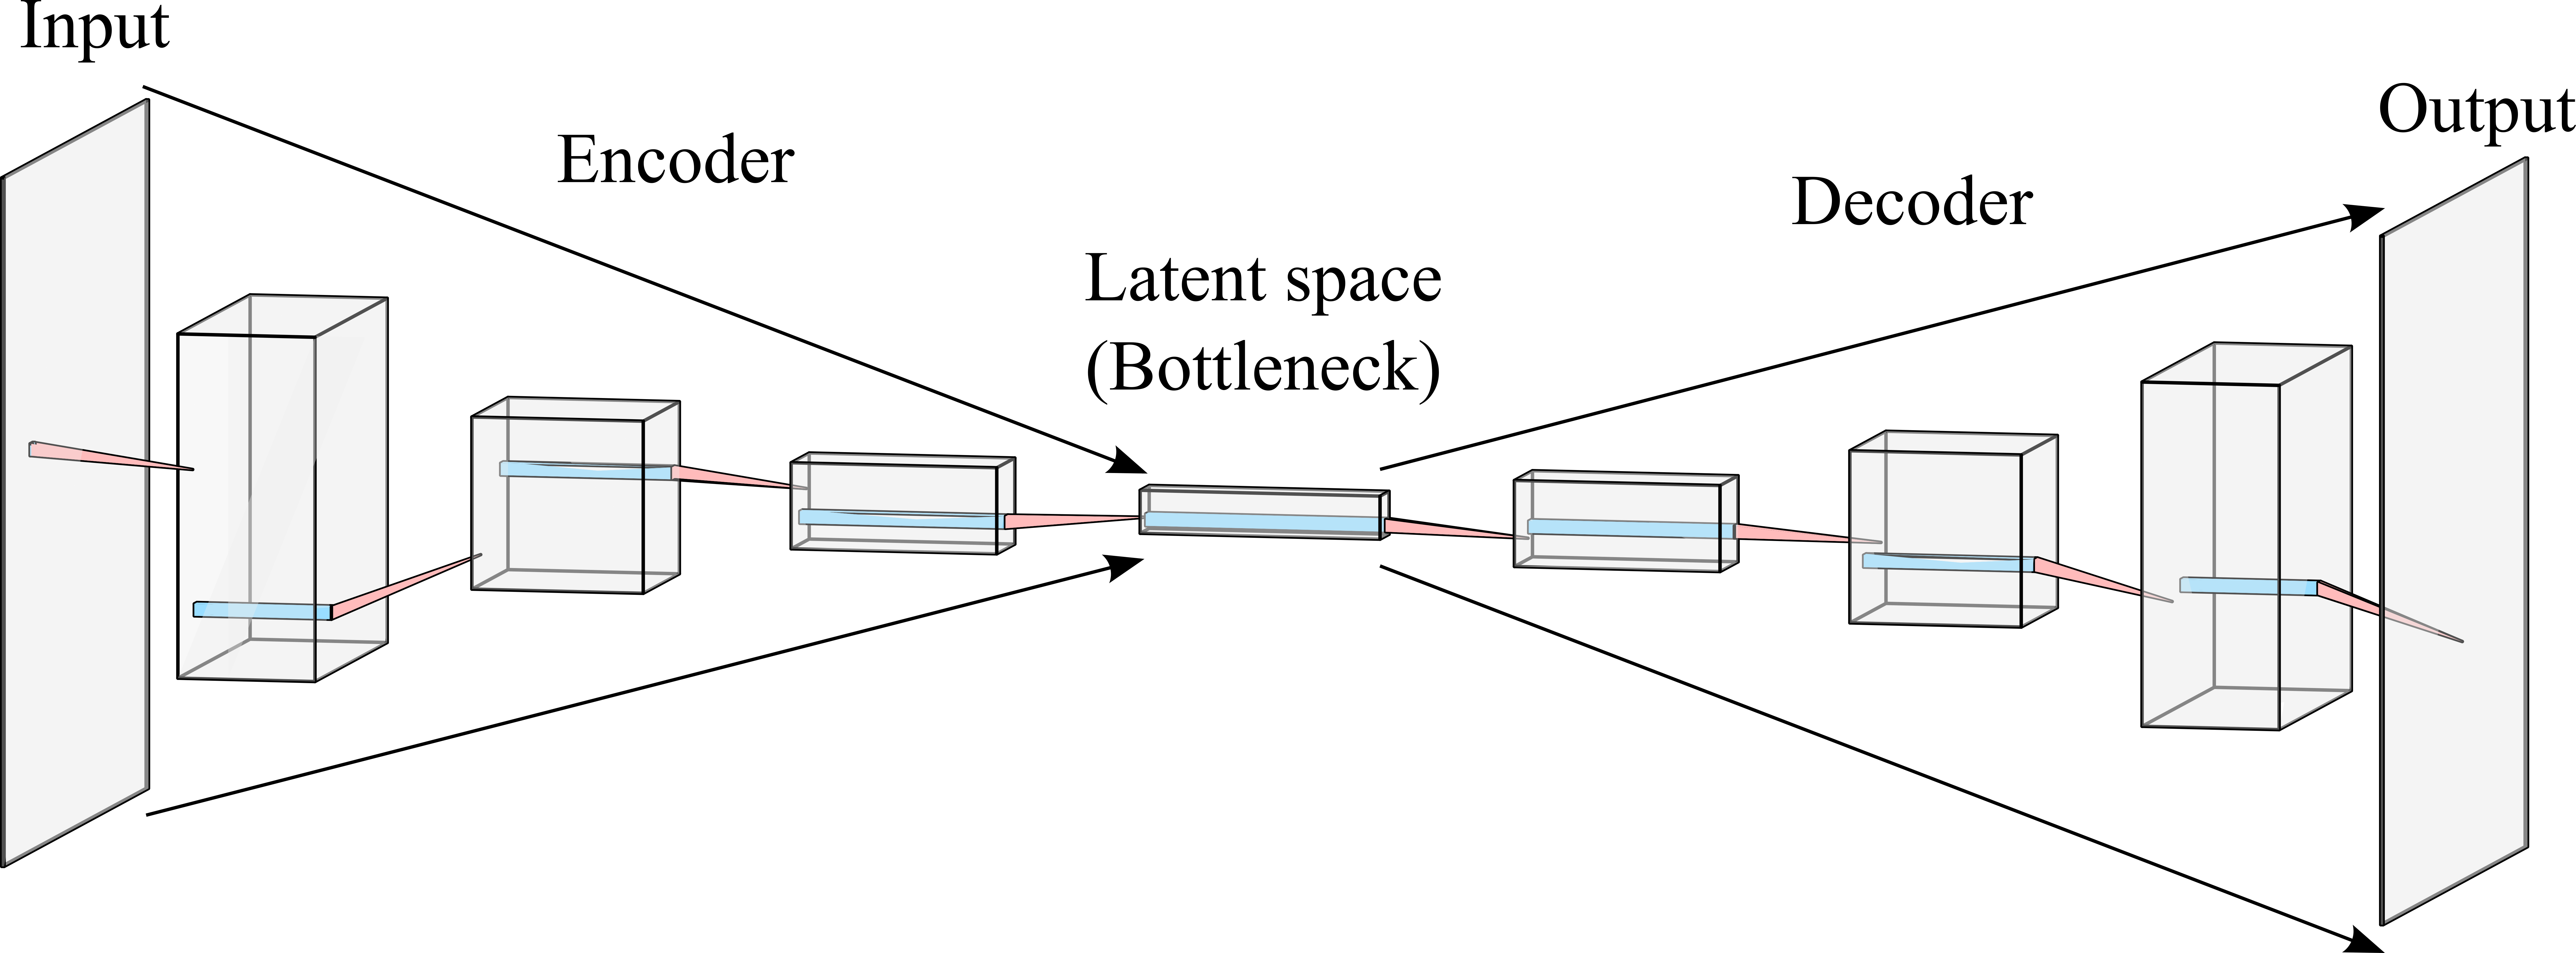
\includegraphics[width=1\textwidth]{nn_encoder_decoder.png}
				\end{figure}	
			\end{column}
		\end{columns}			
	\end{frame}
	%%%%%%%%%%%%%%%%%%%%%%%%%%%%%%%%%%%%%%%%%%%%%%%%%%%%%%%%%%%%%%%%%%%%%%%%%%%%
	\note{
		The encoder-decoder is a well-known architecture used for tasks such as computer vision.
		The encoder aims to produce compressed feature maps from the input image at various scale levels using cascaded convolutions and downsampling operations. 
		The decoder is responsible for upsampling the condensed feature maps in the latent space to the original input shape.		
	}
	
	%%%%%%%%%%%%%%%%%%%%%%%%%%%%%%%%%%%%%%%%%%%%%%%%%%%%%%%%%%%%%%%%%%%%%%%%%%%%
	\begin{frame}{Developing a deep learning model}
		When developing a supervised deep learning model, there are several important considerations to keep in mind:
		\begin{itemize}
			\item Sufficient and Representative Training Data
			\item Data Preprocessing and Augmentation
			\item Model Architecture
			\item Hyperparameter Tuning
			\item Regularization and Overfitting
			\item Choice of Loss Function
			\item Training Strategy
			\item Model Evaluation
			\item Hardware and Computational Resources	
		\end{itemize}
	\end{frame}
	\note{When developing a supervised deep learning model, there are several important considerations to keep in mind:
		
		Sufficient and Representative Training Data: Deep learning models typically require large amounts of labeled training data to generalize well. Ensure that your training dataset is representative of the target population and contains enough diverse examples to capture the underlying patterns effectively.
		
		Data Preprocessing and Augmentation: Preprocess your data appropriately by handling missing values, normalizing features, and addressing class imbalance if present. Consider applying data augmentation techniques, such as rotation, scaling, or flipping, to artificially increase the diversity of your training data.
		
		Model Architecture: Design an appropriate architecture for your deep learning model. Consider the complexity and depth of the model, the type of layers (e.g., convolutional, recurrent, dense), and the use of skip connections or attention mechanisms, depending on the nature of your data and task.
		
		Hyperparameter Tuning: Experiment with different hyperparameter settings to optimize the performance of your model. This includes parameters such as learning rate, batch size, regularization techniques, and activation functions. Utilize techniques like cross-validation or grid search to systematically explore the hyperparameter space.
		
		Regularization and Overfitting: Incorporate regularization techniques, such as dropout, weight decay, or early stopping, to prevent overfitting. Monitor the training and validation loss to ensure your model generalizes well to unseen data.
		
		Choice of Loss Function: Select an appropriate loss function based on the nature of your task. For example, mean squared error (MSE) is commonly used for regression problems, while categorical cross-entropy is often used for multi-class classification tasks.
		
		Training Strategy: Decide on the training strategy for your model. This includes selecting an optimizer (e.g., Adam, SGD), defining the learning rate schedule, and determining the number of epochs or iterations for training. Monitor the training progress using metrics and visualize the learning curves to assess model convergence and performance.
		
		Model Evaluation: Evaluate your model's performance using appropriate evaluation metrics for your task, such as accuracy, precision, recall, F1-score, or mean absolute error (MAE). Additionally, consider cross-validation or using separate validation and test sets to assess the generalization performance of your model.
		
		
		Hardware and Computational Resources: Deep learning models are computationally intensive, so ensure you have access to suitable hardware (e.g., GPUs, TPUs) and sufficient computational resources to train and evaluate your model efficiently.
		
		
		Remember that deep learning models can be complex and require significant computational resources and expertise to develop effectively. It's crucial to iterate, experiment, and fine-tune your model based on empirical observations and domain knowledge to achieve the desired performance.}
	%%%%%%%%%%%%%%%%%%%%%%%%%%%%%%%%%%%%%%%%%%%%%%%%%%%%%%%%%%%%%%%%%%%%%%%%%%%%
	\setcounter{subfigure}{0}
	\section{Case study: Utilisation of AI for delamination identification in CFRP
	}
	%%%%%%%%%%%%%%%%%%%%%%%%%%%%%%%%%%%%%%%%%%%%%%%%%%%%%%%%
	\setcounter{subfigure}{0}
	\begin{frame}{Computer vision}
		\begin{columns}[T]
			\begin{column}[c]{0.27\textwidth}
				\justifying
				\alert {\textbf{Computer vision}} is a field of AI that enables computers and systems to derive meaningful information from digital images, videos and other visual inputs. 
			\end{column}
			\quad
			\begin{column}[c]{0.7\textwidth}
				\begin{figure}
					\centering
					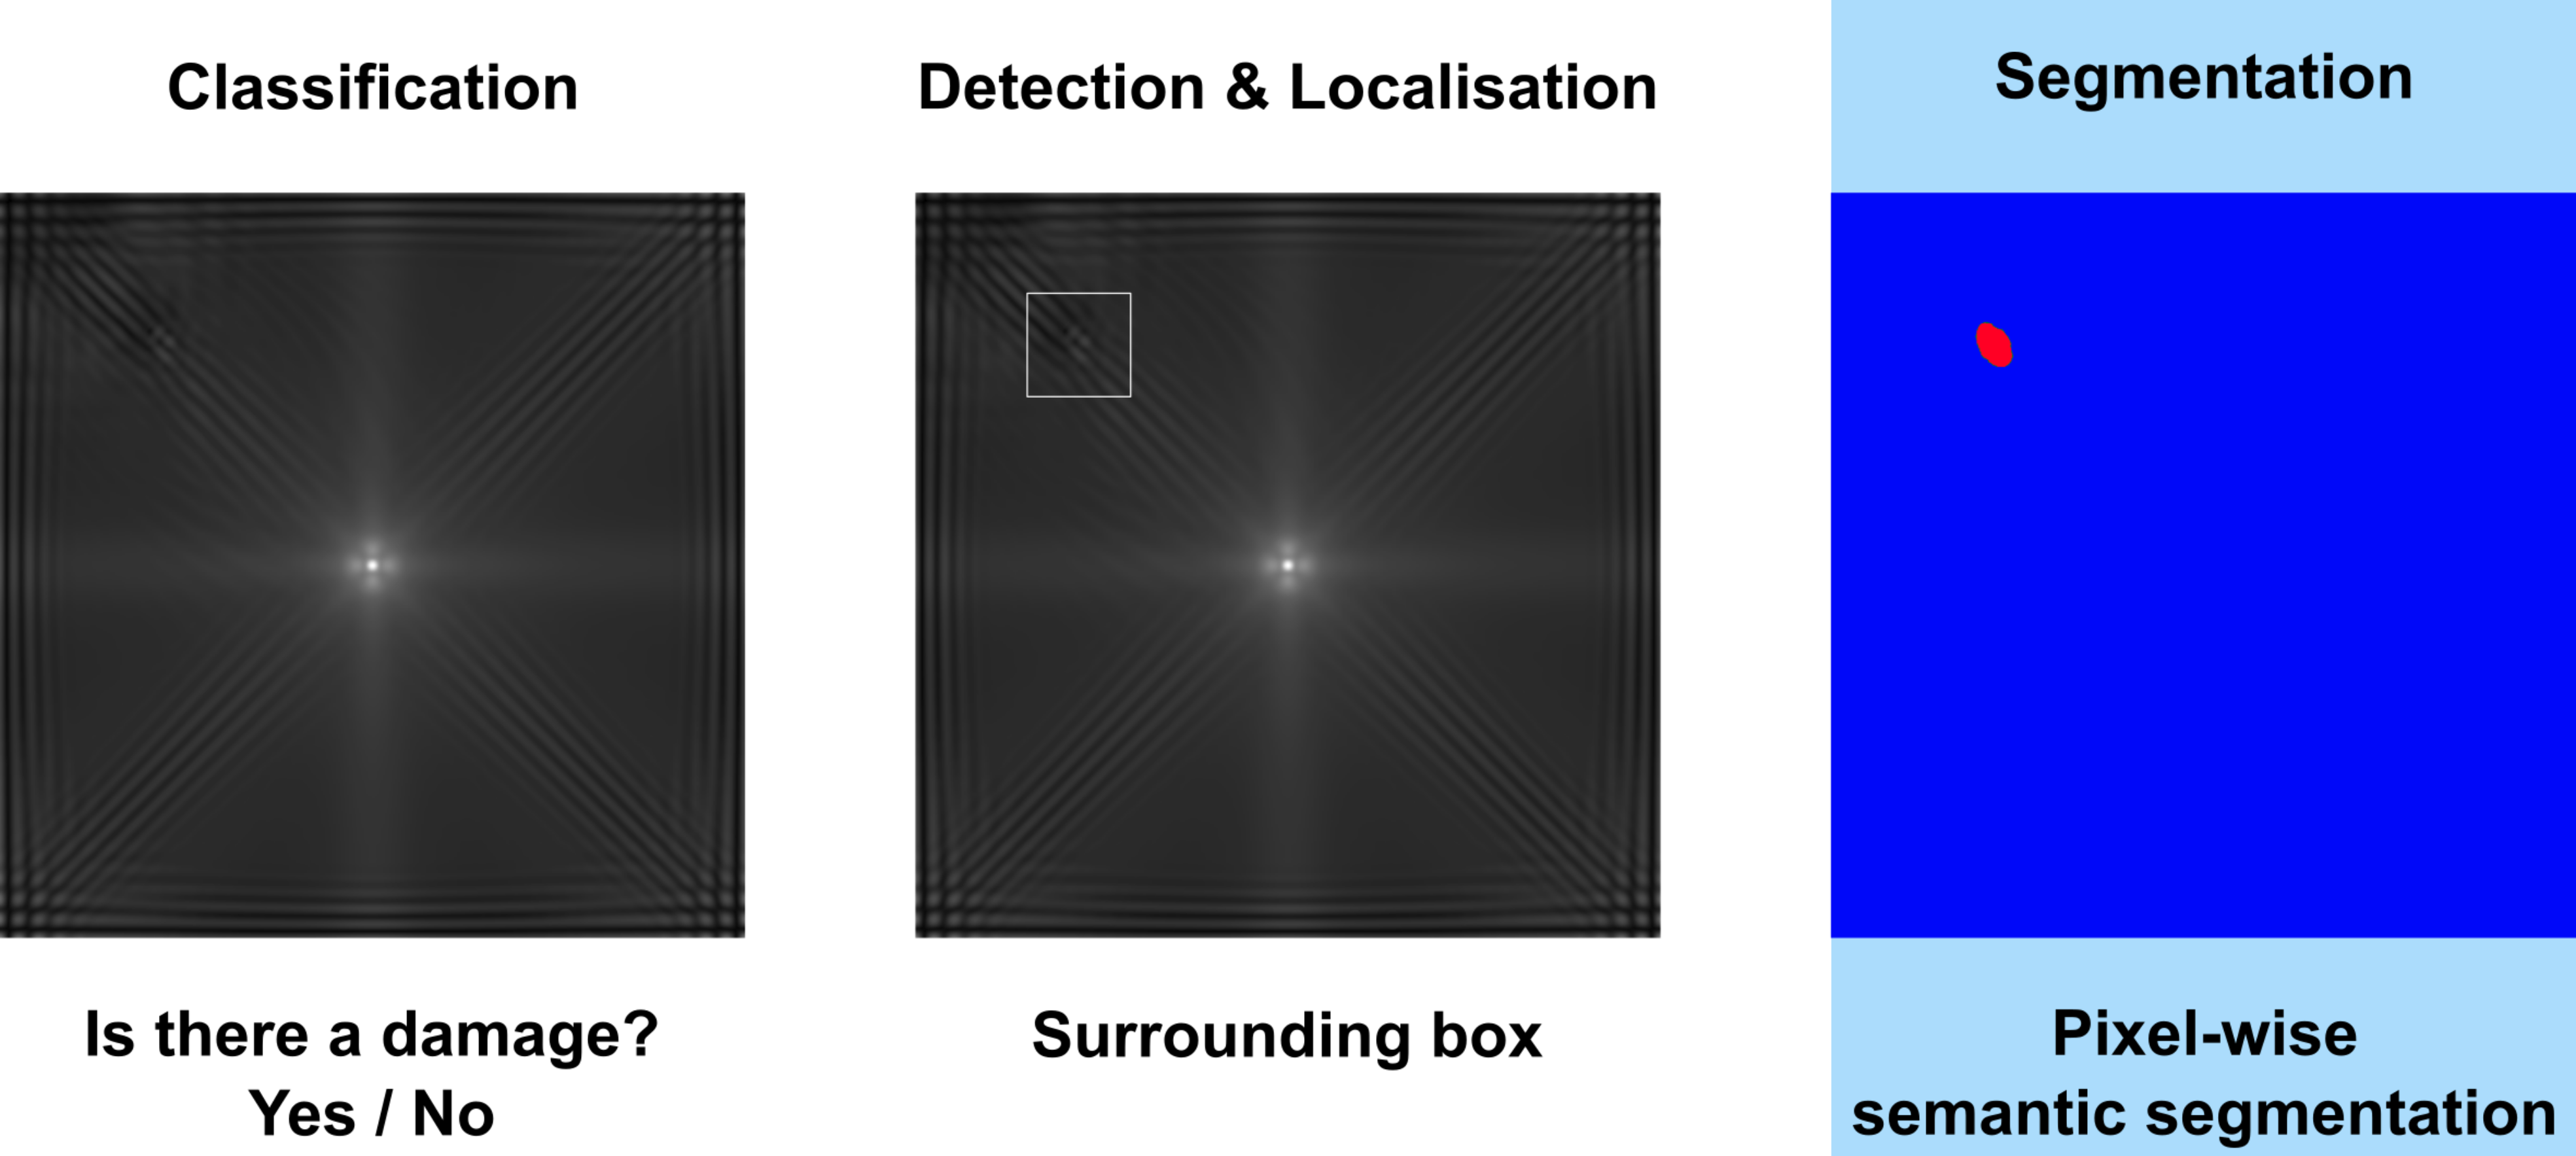
\includegraphics[width=1\textwidth]{computer_vision_tasks.png}
				\end{figure}
			\end{column}
		\end{columns}
	\end{frame}
	%%%%%%%%%%%%%%%%%%%%%%%%%%%%%%%%%%%%%%%%%%%%%%%%%%%%%%%%%%%%%%%%%%%%%%%%%%%%
	\note{
		We now reach an essential concept: computer vision. 
		Computer vision is a subcategory of artificial intelligence that enables computers to obtain meaningful information from visual inputs.
		
		Computer vision has three hierarchical levels: 
		
		The first level performs a classification for the whole input and predicts one output.
		
		The second level classifies and locates the object that we are looking for. 
		
		The ultimate level of computer vision is to perform Pixel-wise segmentation (or semantic segmentation), in which each pixel in the input image is classified into its corresponding class.	
		
		I am using pixel wise image segmentation in my PhD work.
		
	}
	%%%%%%%%%%%%%%%%%%%%%%%%%%%%%%%%%%%%%%%%%%%%%%%%%%%%%%%%%%%%%%%%%%%%%%%%%%%%
	\subsection{Synthetic dataset generation}
	
	%%%%%%%%%%%%%%%%%%%%%%%%%%%%%%%%%%%%%%%%%%%%%%%%%%%%%%%%%%%%%%%%%%%%%%%%%%%%
	\setcounter{subfigure}{0}
	\begin{frame}{Dataset description}
		\begin{columns}[T]
			\begin{column}[t]{0.35\textwidth}
					\begin{itemize}
						\item 475 delamination scenarios
						\item CFRP is made of 8-layers
						\item Delamination modelled between the 3rd and 4th layer
						\item Delamination size min 10 mm, max  40 mm
						\item \textbf{3-months of computing}
					\end{itemize}
			\end{column}
			\begin{column}[t]{0.2\textwidth}
				\begin{figure}[t]
					\centering
					\subfloat[Delamination placement]{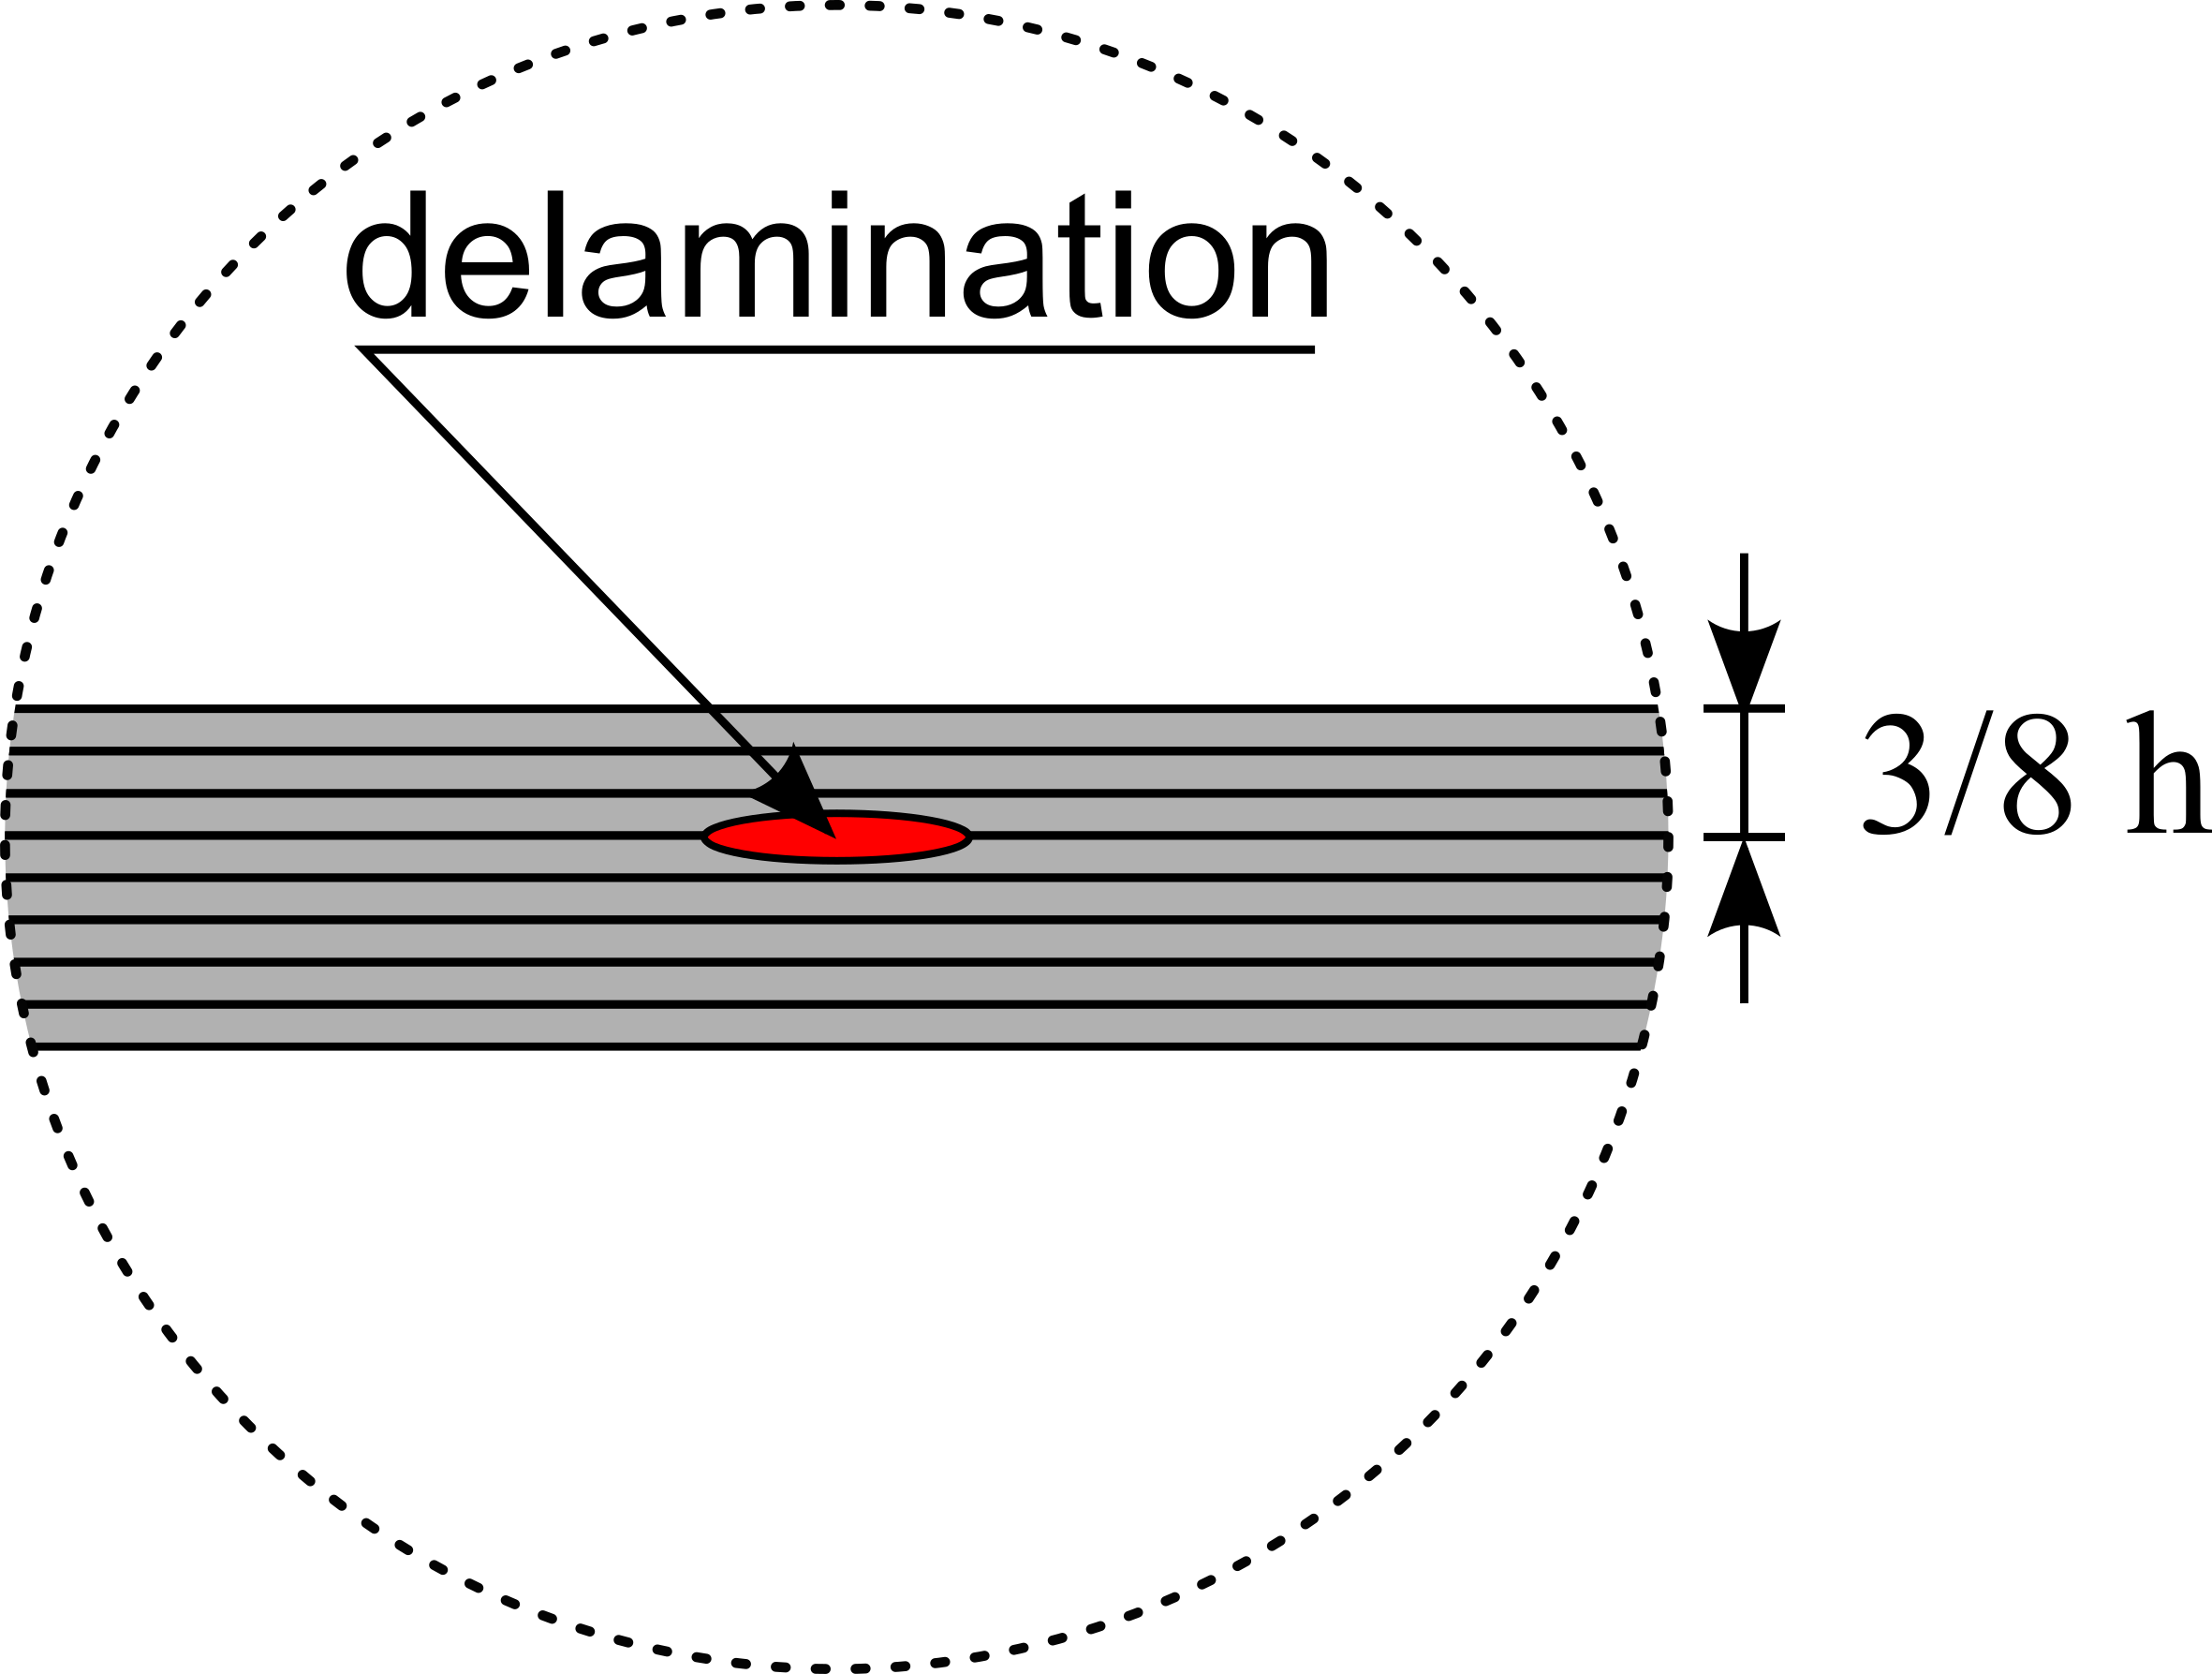
\includegraphics[width=0.95\textwidth]{delamination_placement.png}}
				\end{figure}
			\end{column}
			\begin{column}[t]{0.45\textwidth}
					\begin{figure}[t]					
						\centering						
						\subfloat[Delamination orientation]{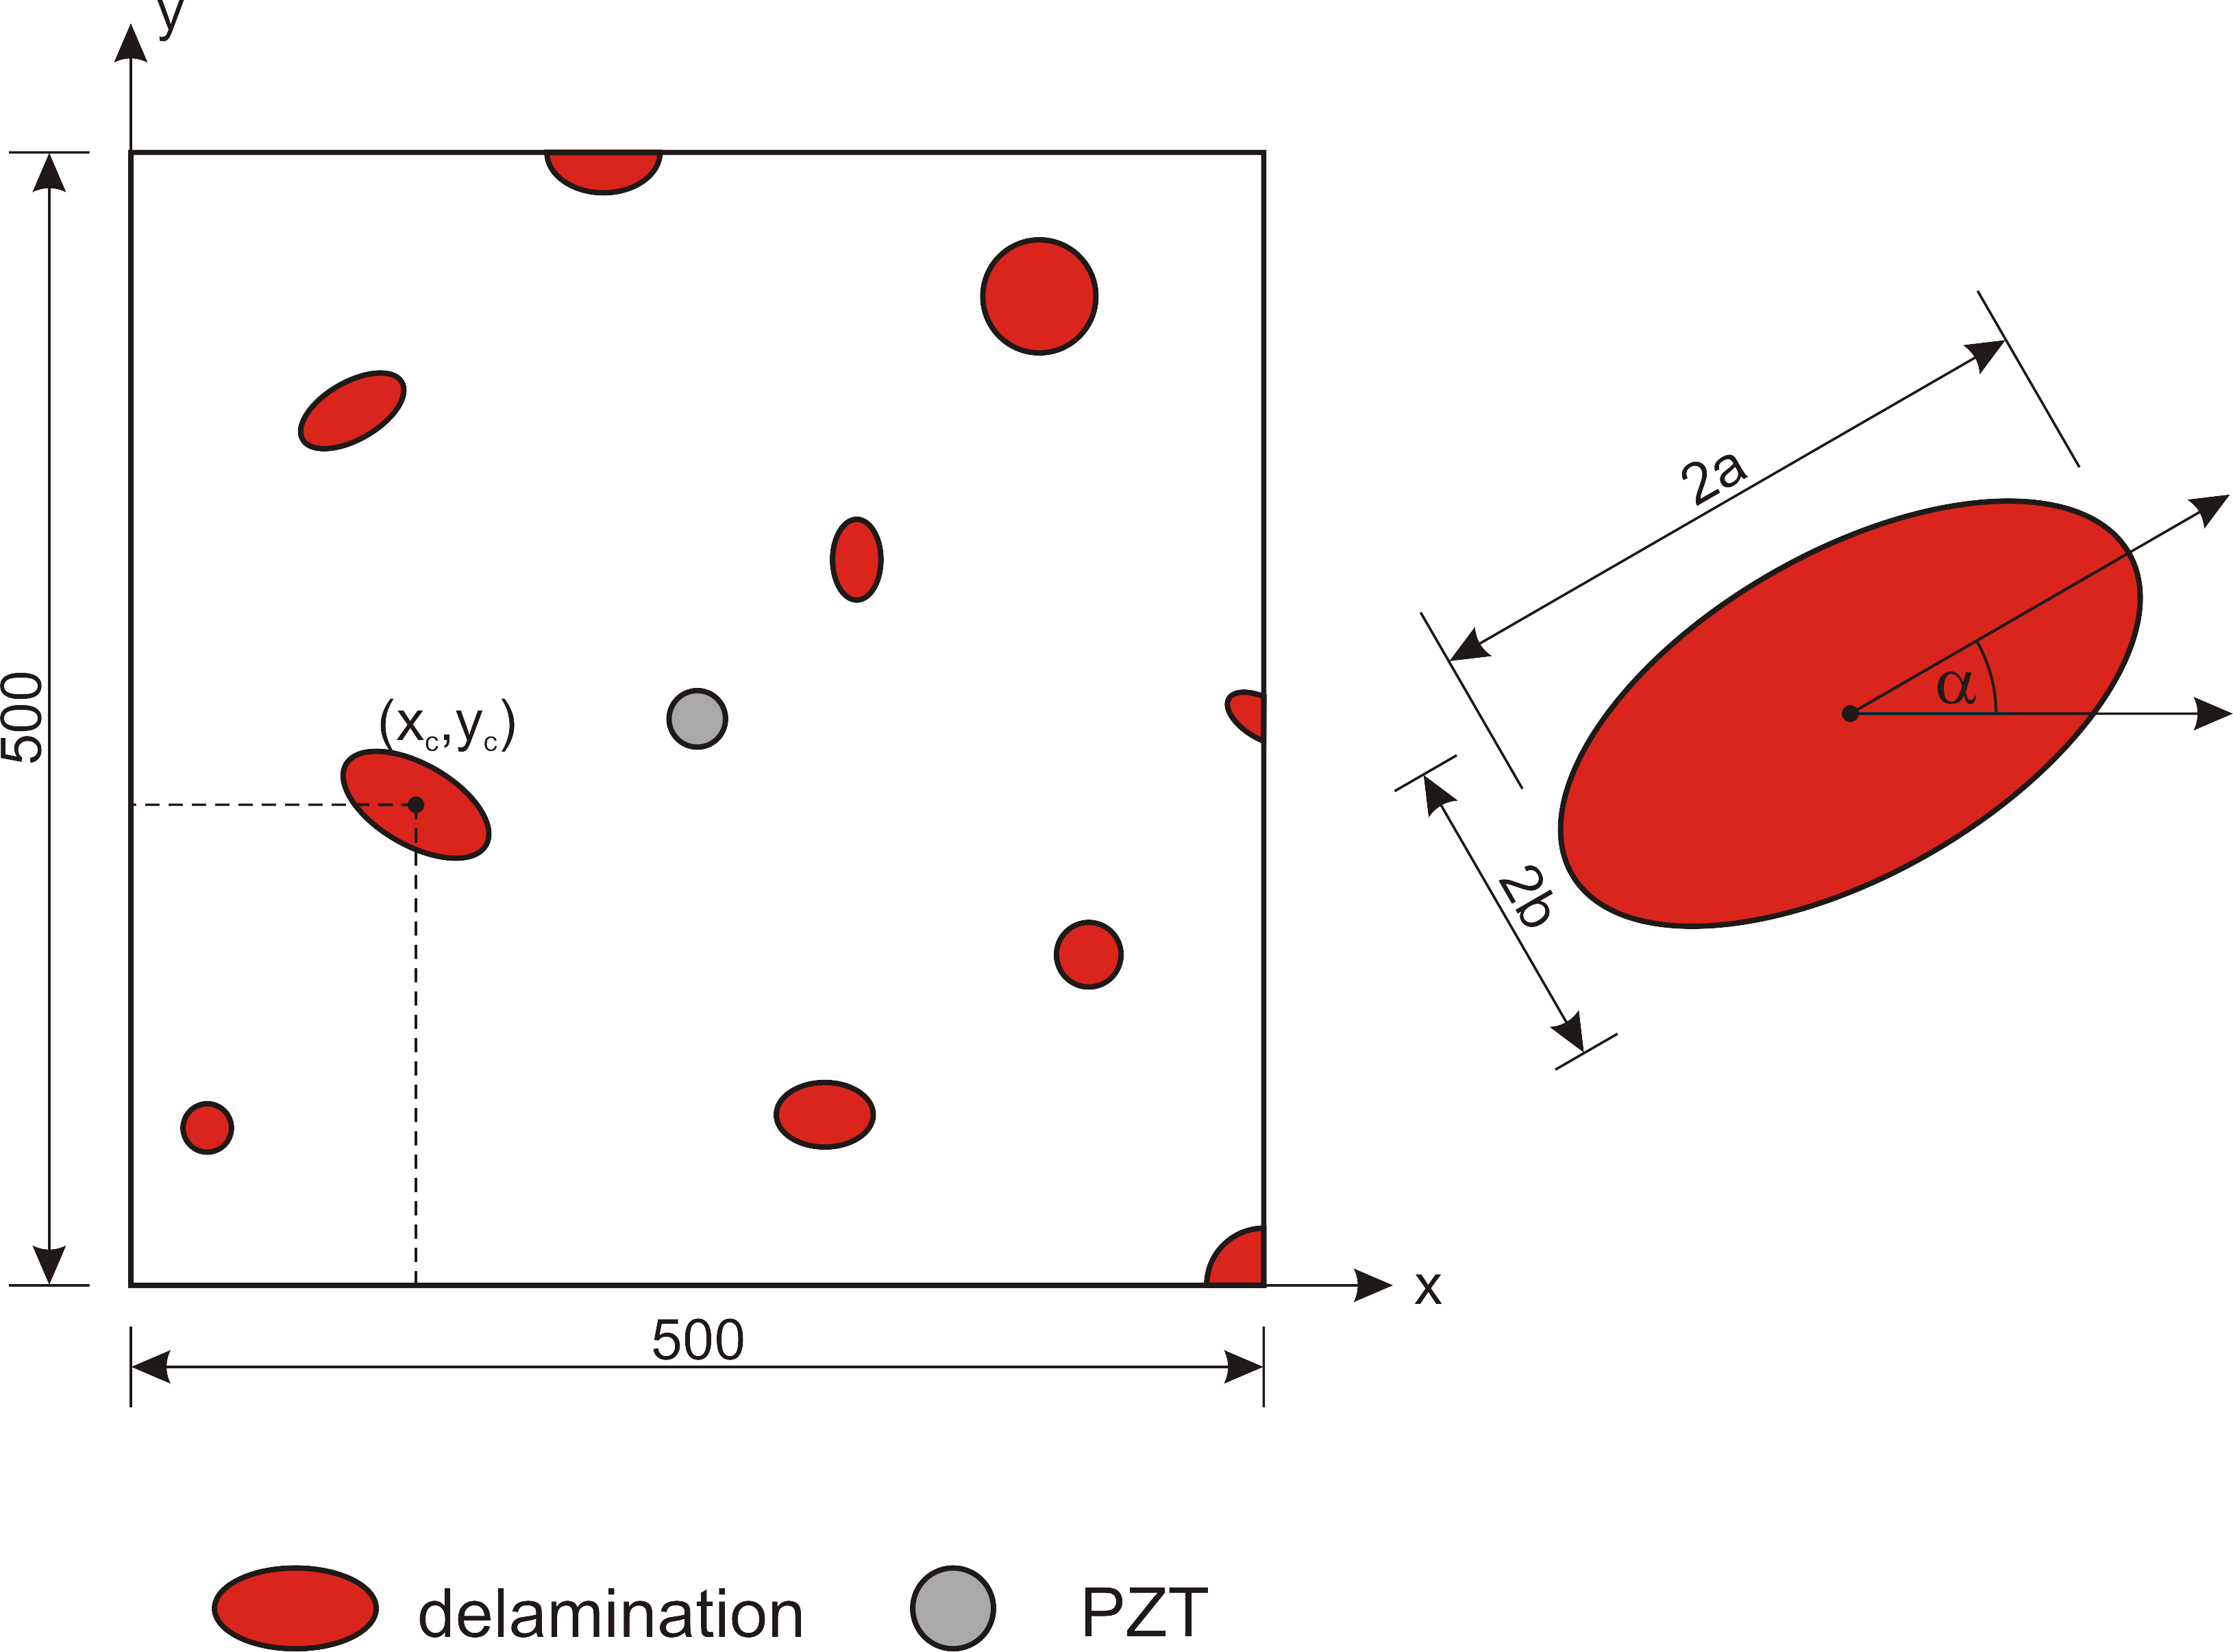
\includegraphics[width=0.95\textwidth]{figure1.png}}					
					\end{figure}
			\end{column}
		\end{columns}
	\end{frame}
	%%%%%%%%%%%%%%%%%%%%%%%%%%%%%%%%%%%%%%%%%%%%%%%%%%%%%%%%%%%%%%%%%%%%%%%%%%%%
	\note{
		The synthetically generated dataset has 475 delamination cases.
		It was assumed that the composite laminate is made of eight layers with a total thickness of 3.9 mm. 
		The delamination was modeled between the third and fourth layers.
		The delamination geometrical size major and minor axes were randomly selected from interval \([10mm,\ 40mm]\). 
		The computation of the dataset took about three months.
	}
	%%%%%%%%%%%%%%%%%%%%%%%%%%%%%%%%%%%%%%%%%%%%%%%%%%%%%%%%%%%%%%%%%%%%%%%%%%%%
	\begin{frame}{The time domain spectral element method}
		\begin{columns}[T]
			\begin{column}{0.47\textwidth}
				\begin{itemize}
					\item Mindlin-Reissner plate theory
					\item Splitting elements and nodes at delamination
					\item GMSH software was used for meshing quads then converted to spectral elements
				\end{itemize}	
				\begin{figure}
					\subfloat{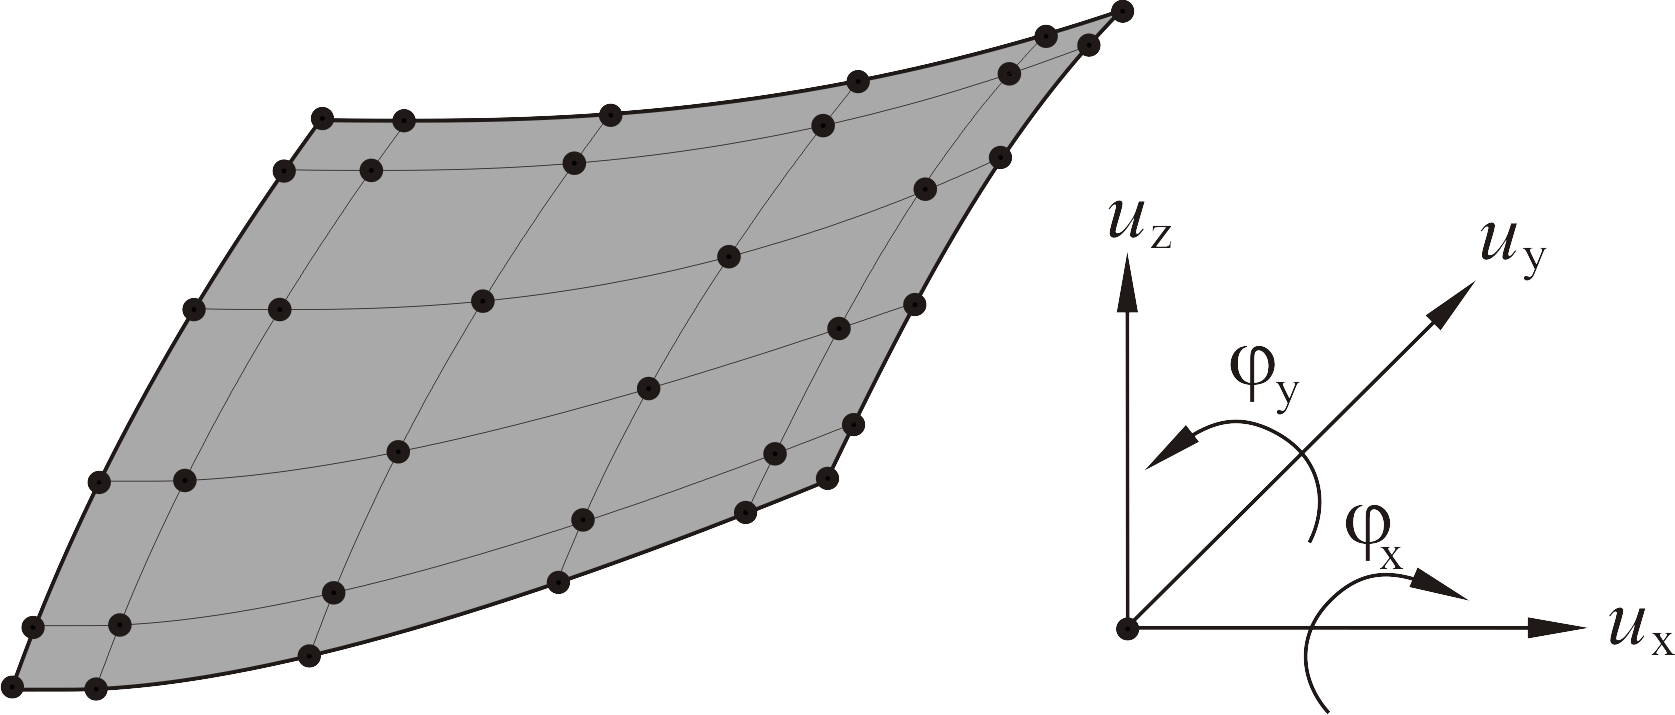
\includegraphics[width=0.9\textwidth]{shell.png}}	
				\end{figure}
			\end{column}
			\begin{column}{0.47\textwidth}	
				\begin{figure}
					\animategraphics[controls,autoplay,loop,width=0.9\textwidth]{1}{/gif_figs/mesh/m1_rand_single_delam_}{1}{20}
				\end{figure}	
			\end{column}
		\end{columns}	
	\end{frame}
	%%%%%%%%%%%%%%%%%%%%%%%%%%%%%%%%%%%%%%%%%%%%%%%%%%%%%%%%%%%%%%%%%%%%%%%%%%%%
	\note{
		To train the supervised deep learning models, a synthetic dataset of propagating waves in carbon fibre-reinforced composite plates was computed by applying the Mindlin-Reissner plate theory and using the parallel implementation of the time domain spectral element method.
		
		For each case, single delamination was modeled by using the method of splitting nodes between appropriate spectral elements.
		
		Essentially, the dataset resembles the particle velocity measurements at the bottom surface of the plate acquired by the SLDV in the transverse direction as a response to the piezoelectric (PZT) excitation at the centre of the plate.		 
	}
	\setcounter{subfigure}{0}
	\begin{frame}{Training Sample case}
		\begin{columns}[T]
			\begin{column}[c]{.32\textwidth}
				\begin{figure}
					\centering
					\animategraphics[autoplay,loop,width=0.95 \textwidth]{16}{figures/gif_figs/7_output/flat_shell_Vz_7_500x500bottom-}{1}{512}
					\caption{Full wavefield $s(x,y,t_k)$}
				\end{figure}
			\end{column}
			\begin{column}[c]{.32\textwidth}
				\begin{figure}
					\centering
					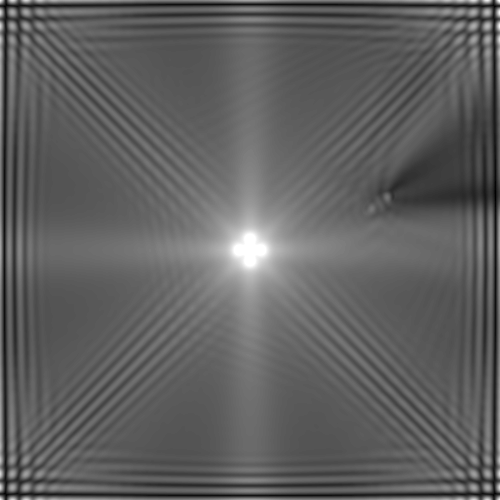
\includegraphics[width=0.95 \textwidth]{RMS_flat_shell_Vz_7_500x500bottom.png}
					\caption{RMS image $\hat{s}(x,y)$}
				\end{figure}
			\end{column}
			\begin{column}[c]{.32\textwidth}
				\begin{figure}
					\centering
					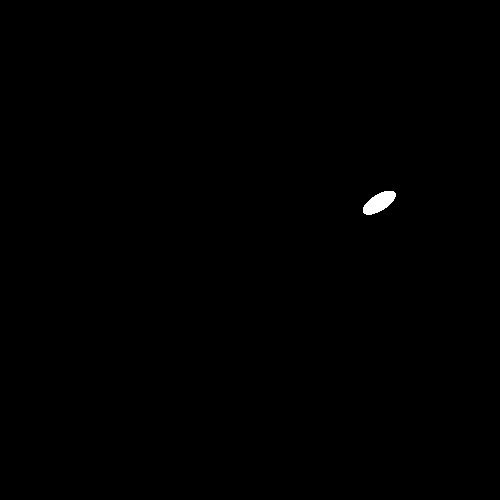
\includegraphics[width=0.95 \textwidth]{m1_rand_single_delam_7.png}
					\caption{Ground truth (label)}
				\end{figure}
			\end{column}
		\end{columns}
		The RMS is defined as:
		\begin{equation*}
			\hat{s}(x,y) = \sqrt{\frac{1}{N}\sum_{k=1}^{N}s(x,y,t_k)^2} 
			\label{eqn:rms} 
		\end{equation*}
	\end{frame}
	%%%%%%%%%%%%%%%%%%%%%%%%%%%%%%%%%%%%%%%%%%%%%%%%%%%%%%%%%%%%%%%%%%%%%%%%%%%%
	\note{
		In this slide, I present a training scenario.
		The animation on the left represents the full wavefield frames, where x and y are the point coordinates, and tk is the time step.
		
		The output of applying the root mean square formula to the full wavefield is shown in the middle figure.
		
		The ground truth label that represents the delamination location and shape is shown on the right.
	}
%%%%%%%%%%%%%%%%%%%%%%%%%%%%%%%%%%%%%%%%%%%%%%%%%%%%%%%%%%%%%%%%%%%%
\subsection{Part I: Delamination identification}
\begin{frame}{Delamination identification approaches}
	\begin{columns}[T]
		\begin{column}[c]{0.47\textwidth}
			\centering
			\textbf{One-to-one \\image-based approach (RMS)} 
			\begin{figure}
				\centering
				\captionsetup{justification=centering}				
				\subfloat[Single input (image)]{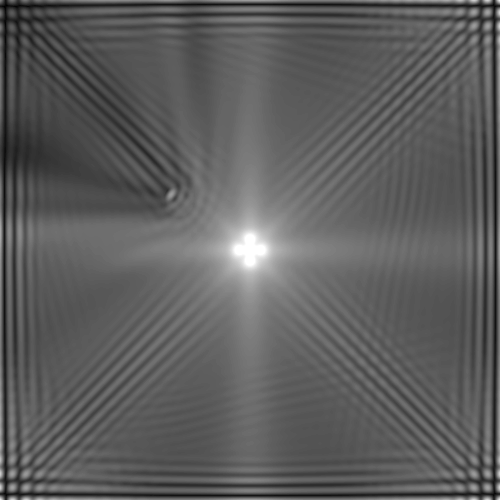
\includegraphics[width=.45\textwidth]{RMS_flat_shell_Vz_381_500x500bottom.png}}\quad
				\subfloat[Single output]{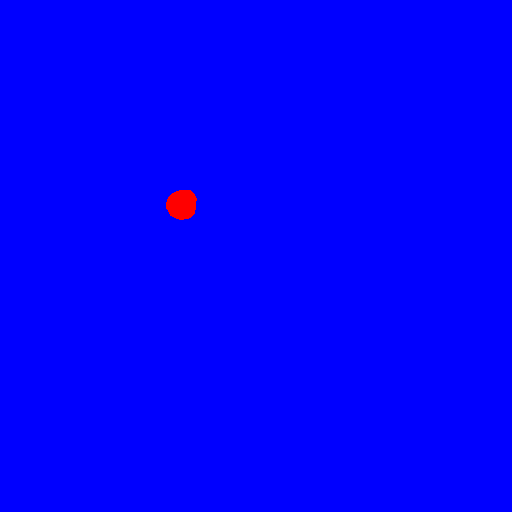
\includegraphics[width=.45\textwidth]{GCN_381.png}}
			\end{figure}
		\end{column}
		\hfill
		\begin{column}[c]{0.47\textwidth}
			\centering
			\textbf{Many-to-one \\animation-based approach}
			\begin{figure}
				\centering
				\captionsetup{justification=centering}					
				\subfloat[Multiple frames (animation)]{\animategraphics[autoplay,loop,width=.45\textwidth]{16}{figures/gif_figs/381_output/output_381-}{1}{512}}\quad
				\subfloat[Single output]{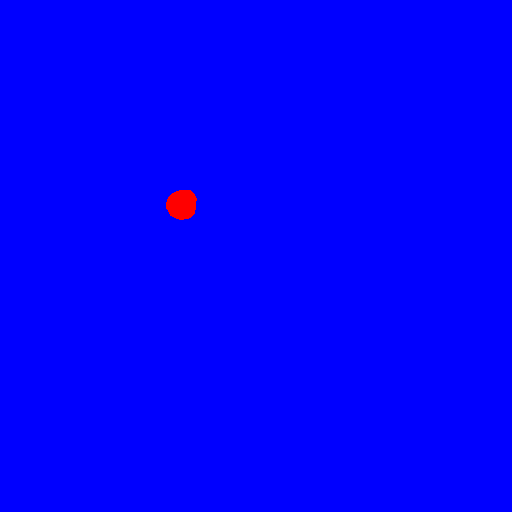
\includegraphics[width=.45\textwidth]{GCN_381.png}}
			\end{figure}
		\end{column}	
	\end{columns}		
\end{frame}	
%%%%%%%%%%%%%%%%%%%%%%%%%%%%%%%%%%%%%%%%%%%%%%%%%%%%%%%%%%%%%%%%%%%%
\note{
	In part, I will present deep learning approaches for delamination identification in composite laminates.
	
	It is important to note how these models perform in an end-to-end fashion.
	
	Accordingly, two approaches for delamination identification based on their inputs were adopted:
	
	\begin{itemize}
		\item the first one is the One-to-one approach (takes one input that is the root mean squared of the full wavefield) and produces one output of damage map)
		\item the second one is the Many-to-one approach (takes animation of Lamb waves propagation as a sequence of frames and produces one output as damage map).
	\end{itemize}	
}
%%%%%%%%%%%%%%%%%%%%%%%%%%%%%%%%%%%%%%%%%%%%%%%%%%%%%%%%%%%%%%%%%%%%
%	\subsection{Developed DL models}
%\begin{frame}{Common deep learning architectures}
%	
%	\begin{column}[t]{0.45\textwidth}
	%		\textbf{RMS based}\\
	%		\begin{itemize}
		%			\item Convolutional neural networks (CNN)
		%			\item Fully convolutional network (FCN)
		%		\end{itemize}
	%	\end{column}
%	\hfill
%	\begin{column}[t]{0.45\textwidth}
	%		\textbf{Full wavefield frames}\\
	%		\begin{itemize}
		%			\item Recurrent neural network (RNN)
		%			\item Long short-term memory (LSTM)
		%			\item ConvLSTM
		%		\end{itemize}
	%	\end{column}
%\end{frame}

%%%%%%%%%%%%%%%%%%%%%%%%%%%%%%%%%%%%%%%%%%%%%%%%%%%%%%%%%%%%%%%%%%%%
\begin{frame}{Developed model for delamination identification}
	\begin{columns}[T]
		\begin{column}[t]{0.45\textwidth}
			\begin{block}{RMS based models}
				\begin{itemize}
					\item VGG 16 encoder-decoder
					\item Res-UNet					
					\item FCN-DenseNet
					\item PSPNet
					\item GCN
				\end{itemize}				
			\end{block}
		\end{column}
		\hfill
		\begin{column}[t]{.50\textwidth}
			\begin{block}{Full wavefield frames based model}					
				\begin{itemize}
					\item Autoencoder ConvLSTM (Convolutional~Long~Short-Term Memory)
				\end{itemize}									
			\end{block}
		\end{column}
	\end{columns}
\end{frame}	
%%%%%%%%%%%%%%%%%%%%%%%%%%%%%%%%%%%%%%%%%%%%%%%%%%%%%%%%%%%%%%%%%%%%
\note{
	
	The developed models based on the RMS image of the full wavefield input are:
	The residual UNet, VGG16 encoder-decoder, fully convolutional dense network (FCN-DenseNet), pyramid scene parsing network (PSPNet), and the global convolutional neural network (GCN)
	
	And the developed model based on the animation of full wavefield frames is Autoencoder ConvLSTM.		
}
%%%%%%%%%%%%%%%%%%%%%%%%%%%%%%%%%%%%%%%%%%%%%%%%%%%%%%%%%%%%%%%%%%%%
\subsection*{RMS based models}	
%%%%%%%%%%%%%%%%%%%%%%%%%%%%%%%%%%%%%%%%%%%%%%%%%%%%%%%%%%%%%%%%%%%%
\setcounter{subfigure}{0}
\begin{frame}{Developed RMS based models}
	\begin{figure}
		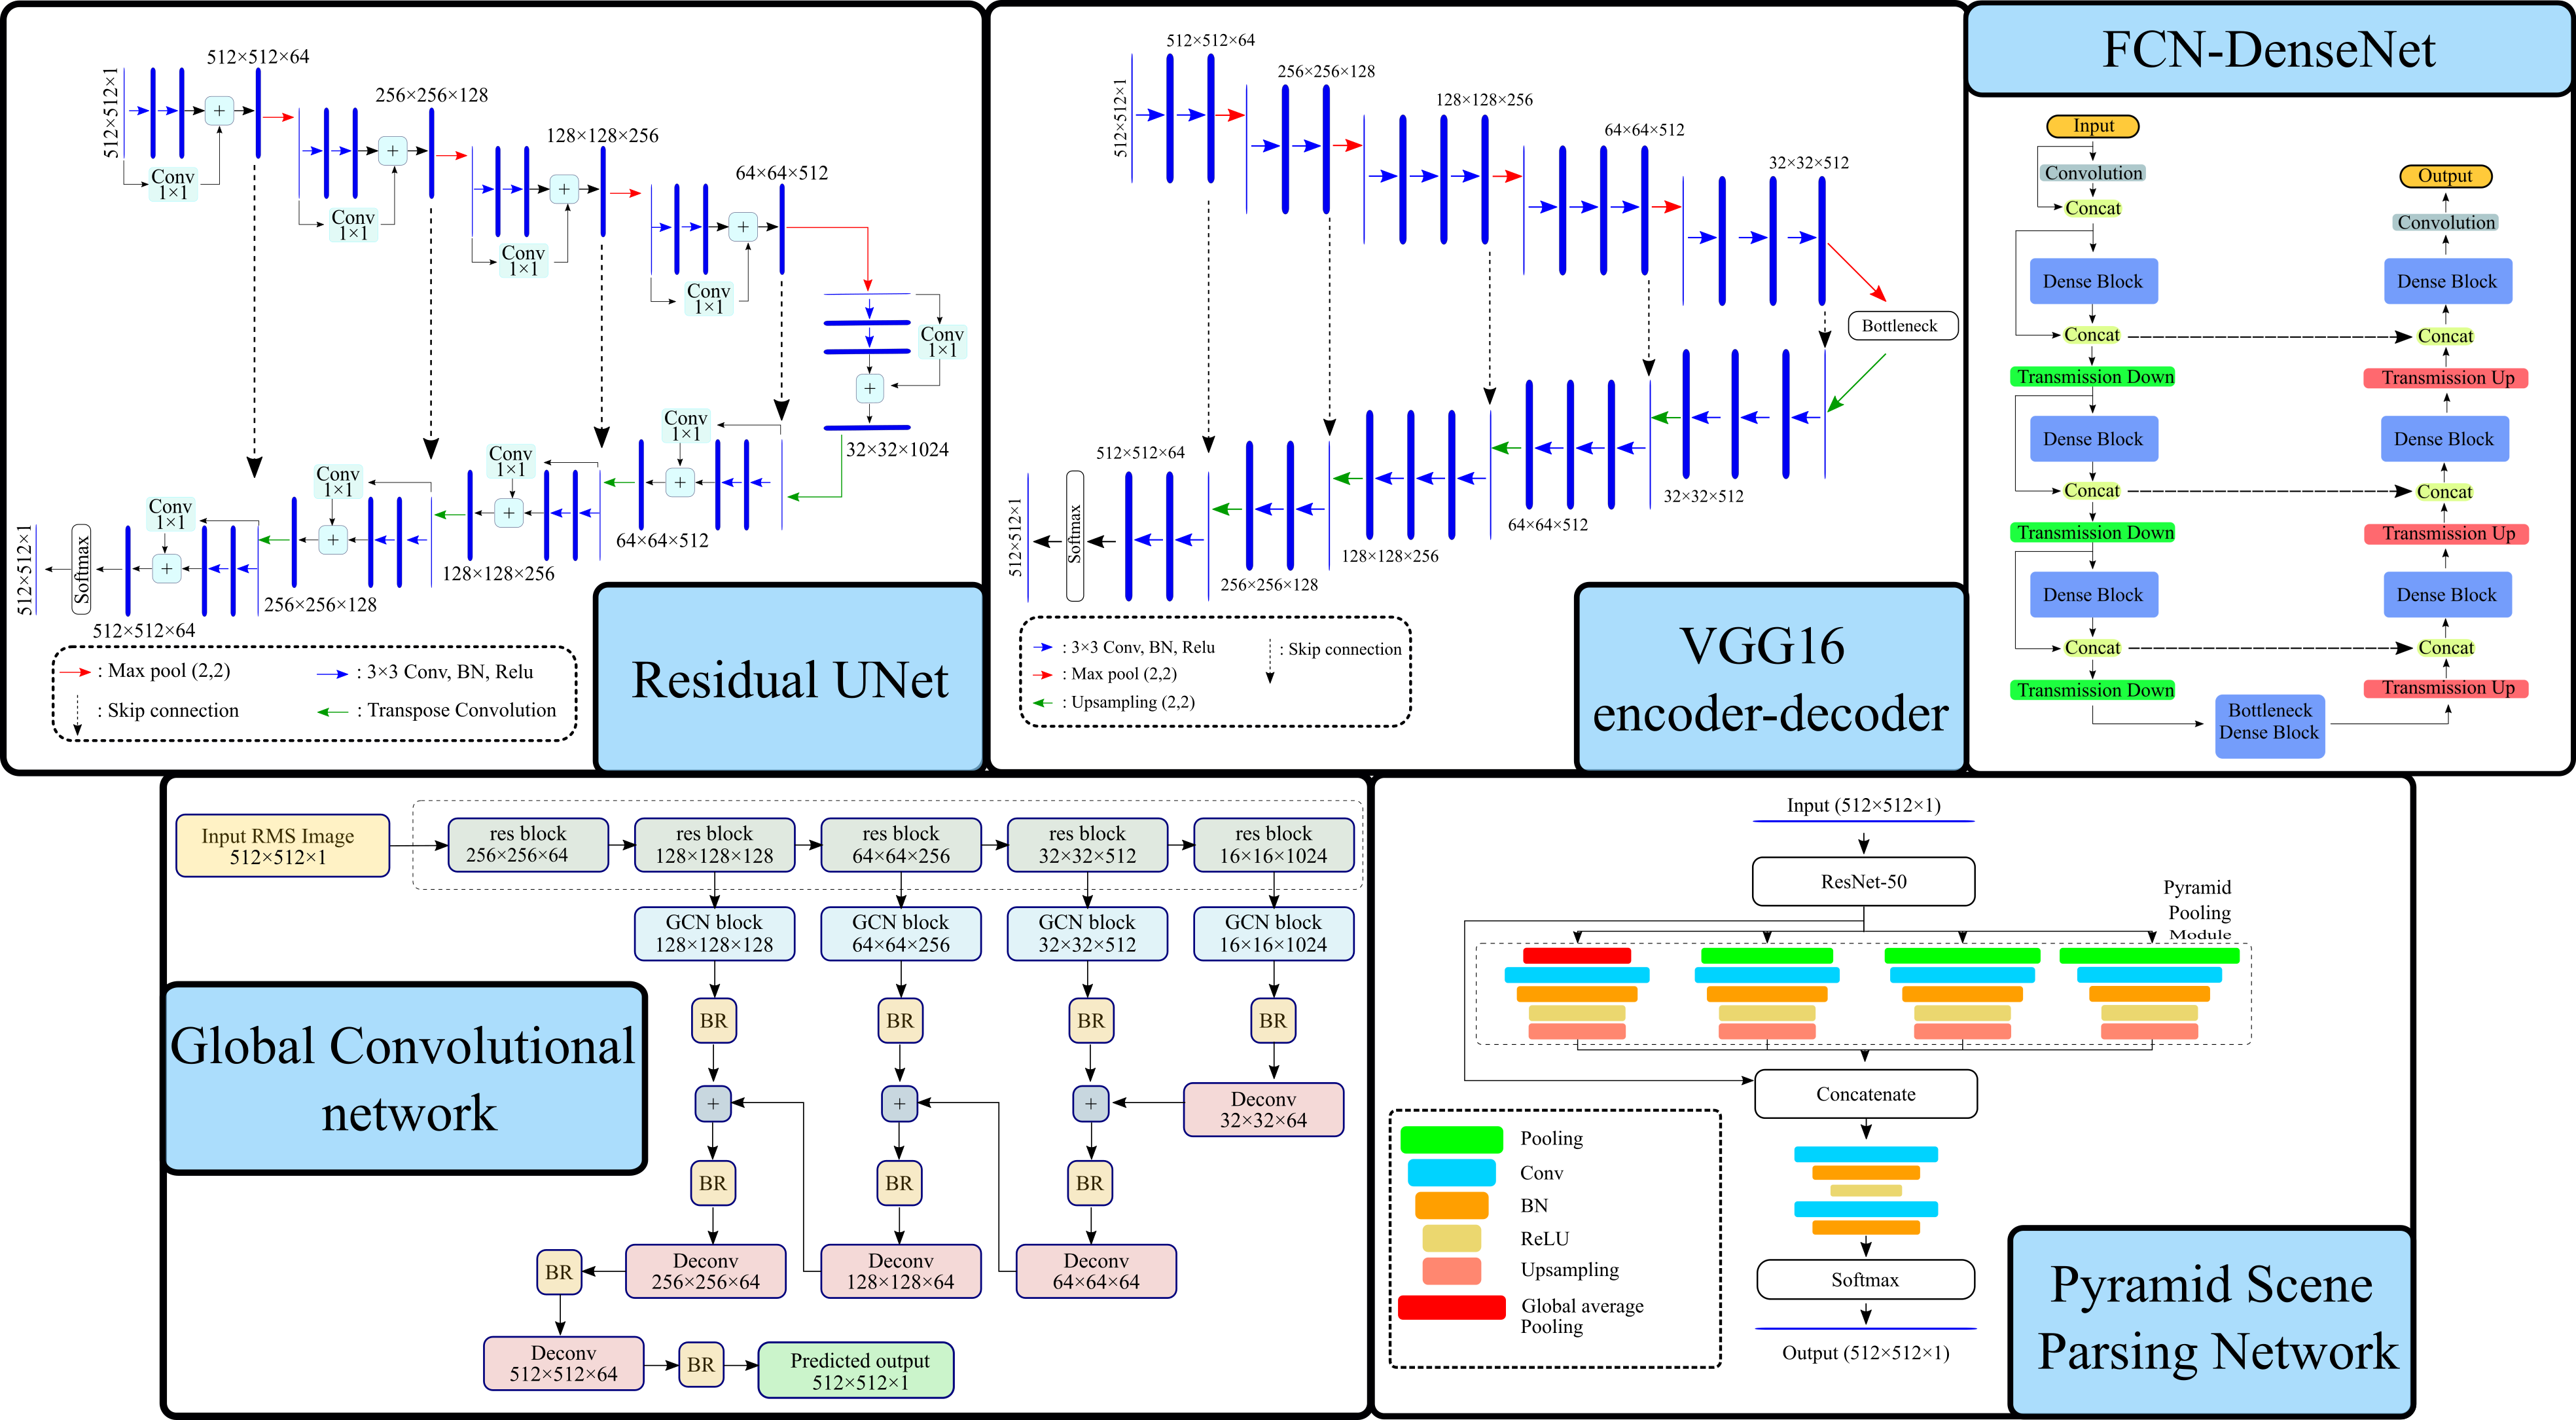
\includegraphics[width=0.95\textwidth]{Developed_rms_models.png}
	\end{figure}
\end{frame}
%%%%%%%%%%%%%%%%%%%%%%%%%%%%%%%%%%%%%%%%%%%%%%%%%%%%%%%%%%%%%%%%%%%%
\setcounter{subfigure}{0}	
%%%%%%%%%%%%%%%%%%%%%%%%%%%%%%%%%%%%%%%%%%%%%%%%%%%%%%%%%%%%%%%%%%%%
\note{
	Here, I present the architectures of all the deep learning models I've created that are based on the RMS image of the full wavefield.
	
	For further details about these models, kindly, I advise you to return to my thesis and my published papers. 
	%		Both the Res-UNet and VGG16 encoder-decoders are autoencoders.
	%		The main difference between them is the additional skip connections that were added to Res-Unet at the encoder and decoder levels. \\
	%		FCN-DenseNet applies an encoder-decoder scheme with skip connections between the encoder and the decoder paths.
	%		The main component in FCN-DenseNet is the dense block. 
	%		The dense block is constructed from a varying number of convolutional layers. 
	%		The purpose of the dense block is to concatenate feature maps of a layer with its output to emphasize spatial details information. \\		
	%		The idea of PSPNet is to provide adequate global contextual information for pixel-level scene parsing by concatenating the local and global features together. 
	%		Hence, a spatial pyramid pooling module was introduced to perform four different pooling levels with four different pool sizes. 
	%		In this way, the pyramid pooling module can capture contextual features at different scales.\\		
	%		GCN addresses the importance of having large kernels at the convolution operations for both localization and classification tasks for semantic segmentation.
}
%%%%%%%%%%%%%%%%%%%%%%%%%%%%%%%%%%%%%%%%%%%%%%%%%%%%%%%%%%%%%%%%%%%%
\setcounter{subfigure}{0}
%%%%%%%%%%%%%%%%%%%%%%%%%%%%%%%%%%%%%%%%%%%%%%%%%%%%%%%%%%%%%%%%%%%%
\subsection*{Full wavefield frames based model}
\begin{frame}{Autoencoder ConvLSTM}
	\begin{figure}[ht!]
		\centering
		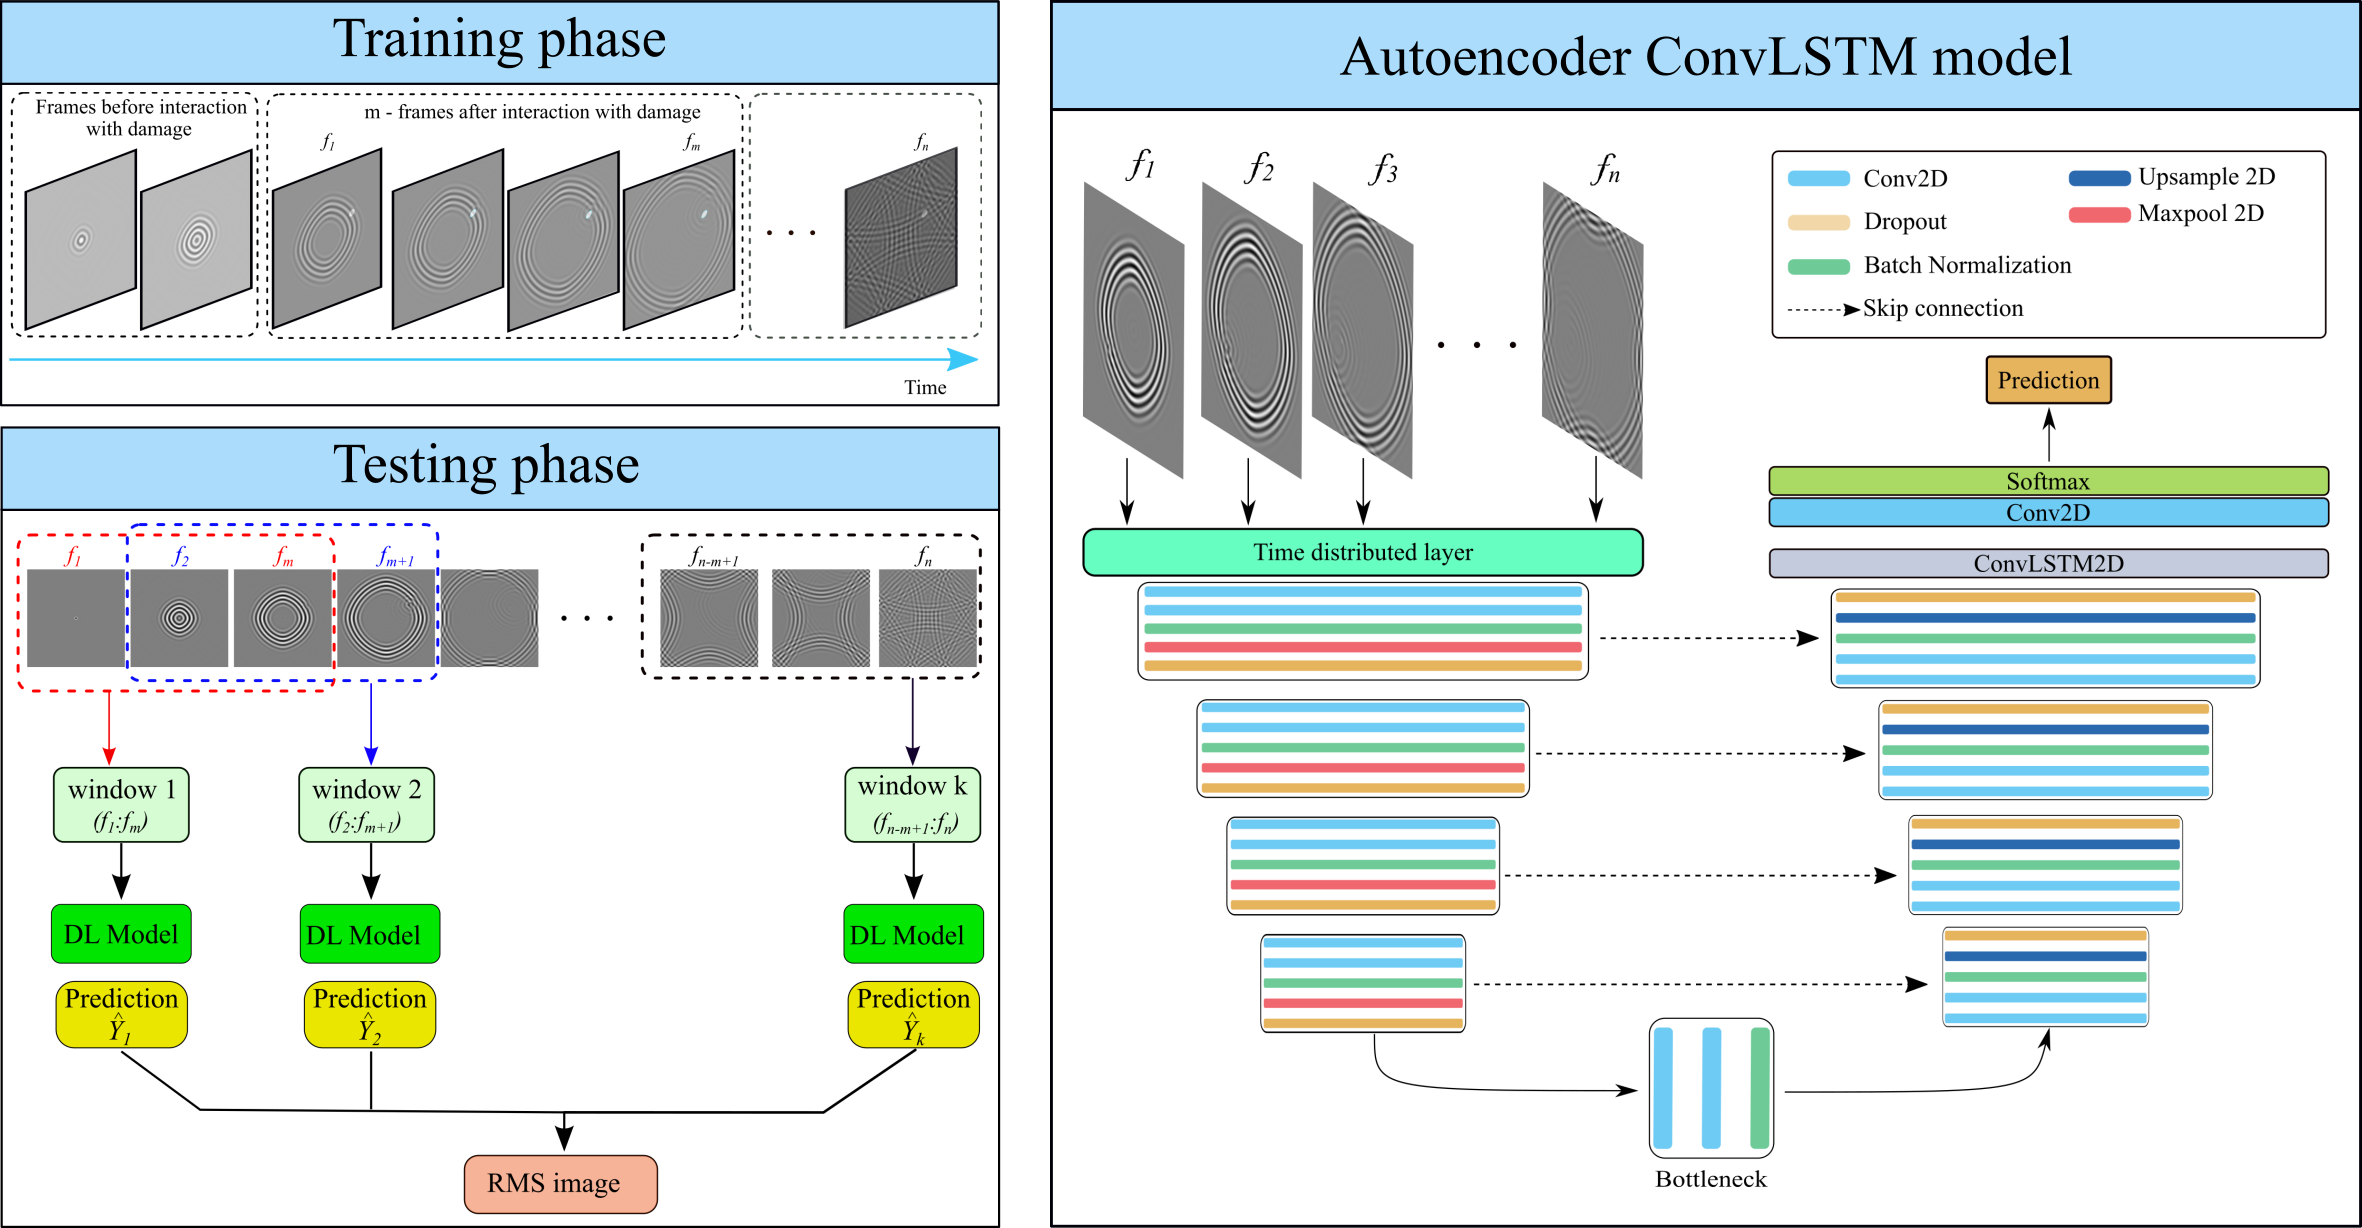
\includegraphics[width=1\textwidth]{figure3.png}
	\end{figure}
\end{frame}
%%%%%%%%%%%%%%%%%%%%%%%%%%%%%%%%%%%%%%%%%%%%%%%%%%%%%%%%%%%%%%%%%%%%
\note{
	Here, I present the developed autoencoder-ConvLSTM model, which takes a sequence of consecutive full wavefield frames of guided wave propagation as an input.
	
	To reduce the training complexity, I used a certain number of frames after the initial interaction of guided waves with the damage, as the delamination location is known.
	
	These selected frames, which contain the required features regarding the delamination shape and location, are fed into an encoder-decoder model at once using a time-distributed layer.
	
	Then, the output of the decoder is forwarded into the ConvLSTM layer, which handles time series data by learning long-term spatiotemporal features.
	
	For real-life situations where the damage location is unknown,  the full wavefield is tested through a sliding window that produces an intermediate output at a time.
	Finally, the root-mean-square formula is applied to all intermediate predictions to obtain the RMS damage map.		
}
%%%%%%%%%%%%%%%%%%%%%%%%%%%%%%%%%%%%%%%%%%%%%%%%%%%%%%%%%%%%%%%%%%%%
\begin{frame}{Evaluation metrics for delamination identification}
	\begin{columns}[T]
		\begin{column}[c]{0.45\textwidth}
			For evaluating delamination identification
			\begin{itemize}
				\item Intersection over Union (IoU): 
				\begin{equation*}
					\textup{IoU}=\frac{Intersection}{Union}=\frac{\hat{Y} \cap Y}{\hat{Y} \cup Y}
					\label{eqn:iou}
				\end{equation*}
				\item Percentage area error $\epsilon$:
				\begin{equation*}
					\epsilon=\frac{|A-\hat{A}|}{A} \times 100\%
					\label{eqn:mean_size_error}
				\end{equation*}
			\end{itemize}
		\end{column}
		\begin{column}[c]{0.45\textwidth}
			\begin{figure}
				\centering
				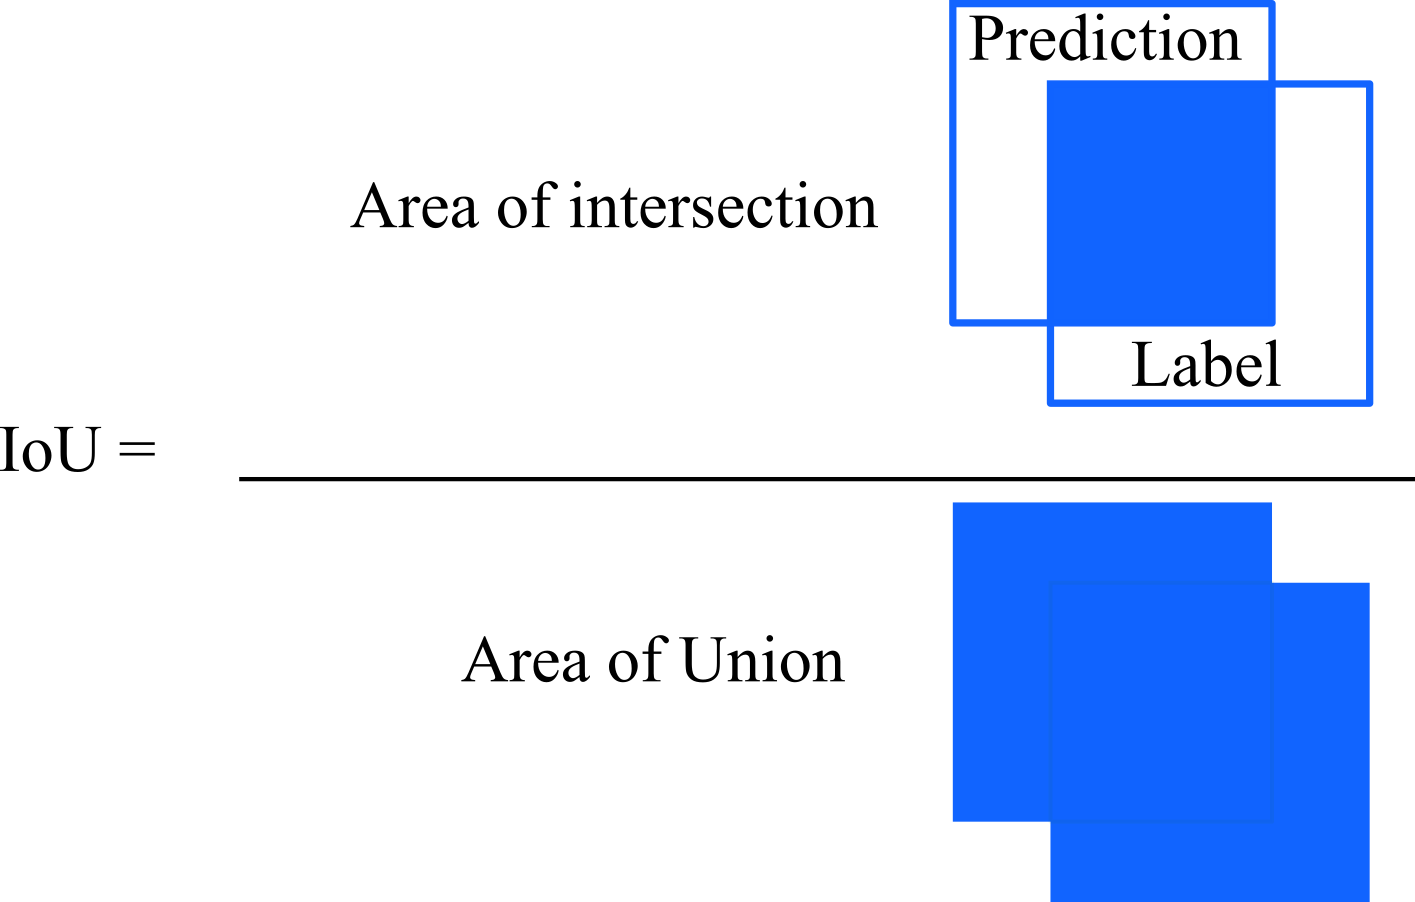
\includegraphics[width=1.0\textwidth]{IoU_figure.png}		
			\end{figure}
		\end{column}
	\end{columns}
\end{frame}
%%%%%%%%%%%%%%%%%%%%%%%%%%%%%%%%%%%%%%%%%%%%%%%%%%%%%%%%%%%%%%%%%%%%
\note{
	Now, to evaluate the developed models for delamination identification, 
	I used two metrics:
	The first metric is the mean intersection over union (also known as the Jaccard index), which calculates the area of intersection between actual and predicted values divided by the union of them.
	The second metric is the percentage area error \(\epsilon\), which calculates the percentage of the difference between actual and predicted areas. 
}
%%%%%%%%%%%%%%%%%%%%%%%%%%%%%%%%%%%%%%%%%%%%%%%%%%%%%%%%%%%%%%%%%%%%
\subsection*{Evaluation: Numerical cases}
%%%%%%%%%%%%%%%%%%%%%%%%%%%%%%%%%%%%%%%%%%%%%%%%%%%%%%%%%%%%%%%%
\begin{frame}{Numerical test cases RMS based models (GCN model)}
	\begin{columns}[T]
		\begin{column}[c]{0.32\textwidth}
			\begin{figure}[c]
				\centering
				\captionsetup{justification=centering}					
				\animategraphics[controls,width=.9\textwidth]{8}{figures/gif_figs/456/intermediate_output-}{0}{82}
				\caption{\(1^{st}\) numerical case, IoU=0.71}
			\end{figure}
		\end{column}
		\hfill
		\begin{column}[c]{0.32\textwidth}
			\begin{figure}[c]
				\centering
				\captionsetup{justification=centering}					
				\animategraphics[controls,width=.9\textwidth]{8}{figures/gif_figs/438/intermediate_output-}{0}{82}
				\caption{\(2^{nd}\) numerical case, IoU=0.72}
			\end{figure}
		\end{column}
		\hfill
		\begin{column}[c]{0.32\textwidth}
			\begin{figure}[c]
				\centering
				\captionsetup{justification=centering}
				
				\animategraphics[controls,width=.9\textwidth]{8}{figures/gif_figs/397/intermediate_output-}{0}{82}
				\caption{\(3^{rd}\) numerical case, IoU=0.86}
			\end{figure}					
		\end{column}
	\end{columns}
\end{frame}
%%%%%%%%%%%%%%%%%%%%%%%%%%%%%%%%%%%%%%%%%%%%%%%%%%%%%%%%%%%%%%%%%%%%
\note{
	This slide shows three numerical samples tested with the GCN model.
	For the first case, the delamination is barely visible by the naked eye, yet the model could identify the delamination with IoU = 0.71.
	For the second case, the IOU = 0.72, and for the third case, the IOU = .86
	Additionally, each animation shows all extracted feature maps from the RMS image input until we get the final prediction of the damage map.
	It's important to notice that GCN can identify the delamination with high accuracy and noise free.			
}
%%%%%%%%%%%%%%%%%%%%%%%%%%%%%%%%%%%%%%%%%%%%%%%%%%%%%%%%%%%%%%%%%%%%
%	\begin{frame}{RMS based: Analysis of numerical cases}
	%		\begin{columns}[T]
		%%				\tiny
		%%				\begin{column}[c]{0.48\textwidth}
			%%					%%%%%%%%%%%%%%%%%%%%%%%%%%%%%%%%%%%%%%%%%%%%%%%%%%%%%%%%%%%%
			%%					\begin{table}[ht!]
				%%						\centering
				%%						\caption{Evaluation metrics of the three numerical cases.}
				%%						\label{tab:RMS_num_cases}
				%%						\begin{tabular}{cccccc}
					%%							\toprule[1.5pt]
					%%							\multirow{2}{*}{Model} & \multirow{2}{*}{case number} & \multicolumn{1}{c}{\multirow{2}{*}{A [mm\textsuperscript{2}]}} & \multicolumn{3}{c}{Predicted output} \\ 
					%%							\cmidrule(lr){4-6} & & & \multicolumn{1}{c}{IoU} & \multicolumn{1}{c}{\(\hat{A}\) [mm\textsuperscript{2}]} & \(\epsilon\) \\
					%%							\midrule
					%%							\multirow{3}{*}{Res-UNet} 							
					%%							& 1 & 257 & \multicolumn{1}{c}{0.45} & \multicolumn{1}{c}{143} & \(44.36\%\) \\ 
					%%							& 2 & 105 & \multicolumn{1}{c}{0.67} & \multicolumn{1}{c}{88} & \(16.19\%\) \\ 
					%%							& 3 & 537 & \multicolumn{1}{c}{0.80} & \multicolumn{1}{c}{478} & \(10.99\%\) \\ 
					%%							\midrule
					%%							\multirow{3}{*}{VGG16 encoder-decoder} 
					%%							& 1 & 257 & \multicolumn{1}{c}{0.69} & \multicolumn{1}{c}{203} & \(21.01\%\) \\ 
					%%							& 2 & 105 & \multicolumn{1}{c}{0.75} & \multicolumn{1}{c}{117} & \(11.43\%\) \\ 
					%%							& 3 & 537 & \multicolumn{1}{c}{0.65} & \multicolumn{1}{c}{385} & \(28.31\%\) \\ 
					%%							\midrule
					%%							\multirow{3}{*}{FCN-DenseNet} 
					%%							& 1 & 257 & \multicolumn{1}{c}{0.52} & \multicolumn{1}{c}{505} & \(96.50\%\) \\ 
					%%							& 2 & 105 & \multicolumn{1}{c}{0.66} & \multicolumn{1}{c}{118} & \(12.38\%\) \\ 
					%%							& 3 & 537 & \multicolumn{1}{c}{0.72} & \multicolumn{1}{c}{815} & \(51.77\%\) \\ 
					%%							\midrule
					%%							\multirow{3}{*}{PSPNet} 
					%%							& 1 & 257 & \multicolumn{1}{c}{0.00} & \multicolumn{1}{c}{0} & \(-\%\) \\ 
					%%							& 2 & 105 & \multicolumn{1}{c}{0.44} & \multicolumn{1}{c}{156} & \(48.57\%\) \\ 
					%%							& 3 & 537 & \multicolumn{1}{c}{0.77} & \multicolumn{1}{c}{610} & \(13.59\%\) \\ 
					%%							\midrule
					%%							\multirow{3}{*}{GCN} 
					%%							& 1 & 257 & \multicolumn{1}{c}{0.71} & \multicolumn{1}{c}{215} & \(16.34\%\) \\ 
					%%							& 2 & 105 & \multicolumn{1}{c}{0.72} & \multicolumn{1}{c}{177} & \(68.57\%\) \\ 
					%%							& 3 & 537 & \multicolumn{1}{c}{0.86} & \multicolumn{1}{c}{523} & \(2.61\%\) \\ 
					%%							\bottomrule[1.5pt]
					%%						\end{tabular}	
				%%					\end{table}
			%	 %%%%%%%%%%%%%%%%%%%%%%%%%%%%%%%%%%%%%%%%%%%%%%%%%%%%%%%%%%%%%%%
			%% \end{column}
		%%		\hfill
		%		\begin{column}[c]{0.9\textwidth}
			%			\begin{table}[ht!]
				%				\centering
				%				\caption{Analysis of numerical cases.}
				%				\label{tab:table_all_numerical_cases}	
				%				\begin{tabular}{lcc}
					%					\toprule[1.5pt]
					%					Model & mean IoU & max IoU \\ 
					%					\midrule 
					%					Res-UNet & \(0.66\) & \(0.89\) \\ 
					%					VGG16 encoder-decoder & \(0.57\) & \(0.84\) \\ 
					%					FCN-DenseNet & \(0.68\) & \(0.92\) \\ 
					%					PSPNet & \(0.55\) & \(0.91\) \\ 
					%					GCN & \textbf{\(0.76\)} & \textbf{\(0.93\)} \\ 
					%					\bottomrule[1.5pt]
					%				\end{tabular}
				%			\end{table}
			%		\end{column}
		%		\end{columns}
	%	\end{frame}
%%%%%%%%%%%%%%%%%%%%%%%%%%%%%%%%%%%%%%%%%%%%%%%%%%%%%%%%%%%%%%%%%%%%
%	\note{
	%		The table presents the mean and maximum values calculated for the previously unseen numerical test set for all RMS-based models. 
	%		It also shows that all models have a relatively high value, indicating their ability to detect and localize the delamination.
	%		However, the best performance was achieved by the GCN model.
	%	}
%%%%%%%%%%%%%%%%%%%%%%%%%%%%%%%%%%%%%%%%%%%%%%%%%%%%%%%%%%%%%%%%%%%%
\begin{frame}{Numerical test cases animation of Lamb waves}
	\setcounter{subfigure}{0}
	\only<1>{
		\begin{alertblock}{First test case}
			\begin{figure}
				\centering
				\captionsetup{justification=centering}
				\subfloat[Full wavefield (512 frames)]{\animategraphics[autoplay,loop,height=3cm,keepaspectratio]{32}{figures/gif_figs/381_output/output_381-}{1}{512}}\quad
				\subfloat[Intermediate outputs]{\animategraphics[autoplay,loop,height=3cm,keepaspectratio]{31}{figures/gif_figs/Numerical_case_381/num_case_381_frame_num-}{0}{487}}\quad
				\subfloat[RMS (damage map)]{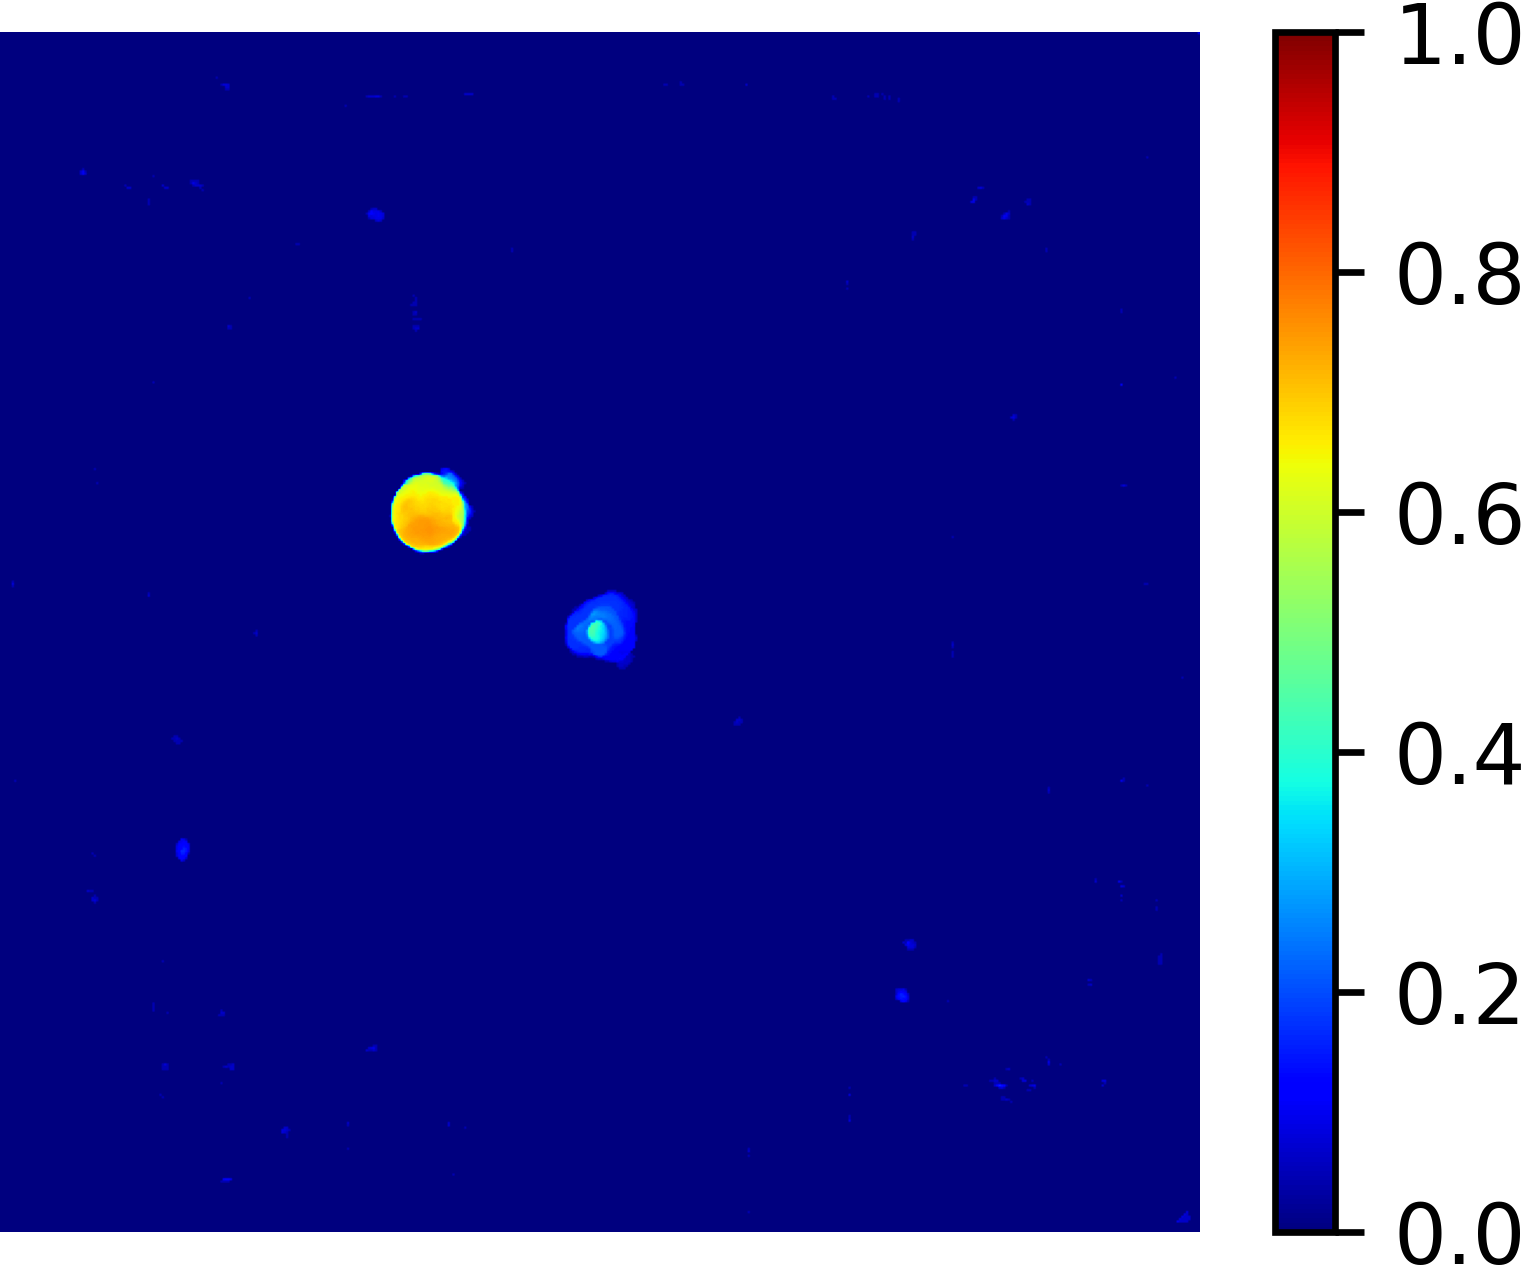
\includegraphics[height=3.05cm,keepaspectratio]{figures/RMS_Ijjeh_num_case_381.png}}\quad
				\subfloat[Binary RMS, IoU= 0.88]{
\includegraphics[height=3cm,keepaspectratio]{figures/Binary_RMS_Ijjeh_num_case381_.png}}\quad
			\end{figure}
	\end{alertblock}}
	\setcounter{subfigure}{0}
	\only<2>{
		\begin{alertblock}{Second test case}
			\begin{figure}
				\centering
				\captionsetup{justification=centering}
				\subfloat[Full wavefield (512 frames)]{\animategraphics[autoplay,loop,height=3cm,keepaspectratio]{32}{figures/gif_figs/385_output/output_385-}{1}{512}}\quad		
				\subfloat[Intermediate outputs]{\animategraphics[autoplay,loop,height=3cm,keepaspectratio]{31}{figures/gif_figs/Numerical_case_385/num_case_385_frame_num-}{0}{487}}\quad			
				\subfloat[RMS (damage map)]{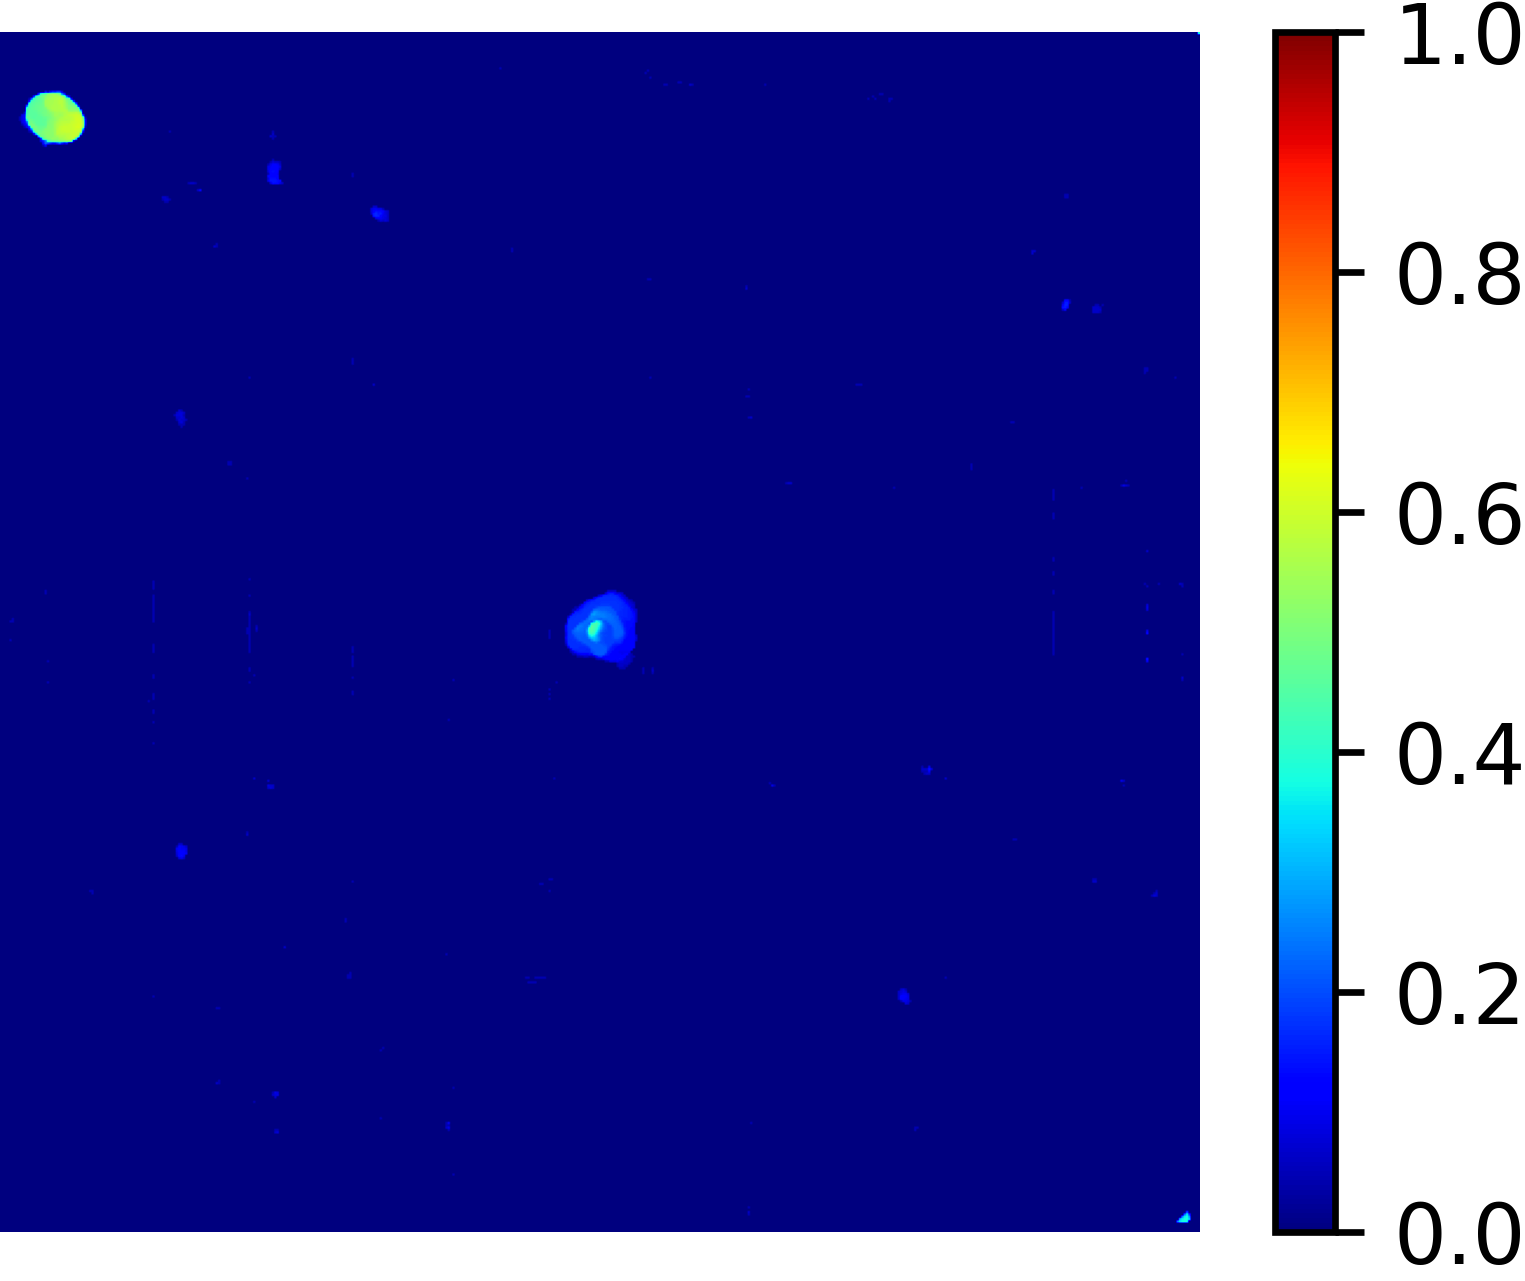
\includegraphics[height=3.05cm,keepaspectratio]{figures/RMS_Ijjeh_num_case_385.png}}\quad
				\subfloat[Binary RMS, IoU= 0.58]{
\includegraphics[height=3cm,keepaspectratio]{figures/Binary_RMS_Ijjeh_num_case385_.png}}
			\end{figure}
	\end{alertblock}}
	\setcounter{subfigure}{0}
	\only<3>{
		\begin{alertblock}{Third test case}
			\begin{figure}
				\centering
				\captionsetup{justification=centering}
				\subfloat[Full wavefield (512 frames)]{\animategraphics[autoplay,loop,height=3cm,keepaspectratio]{32}{figures/gif_figs/394_output/output_394-}{1}{512}}\quad
				\subfloat[Intermediate outputs]{\animategraphics[autoplay,loop,height=3cm,keepaspectratio]{31}{figures/gif_figs/Numerical_case_394/num_case_394_frame_num-}{0}{487}}\quad
				\subfloat[RMS (damage map)]{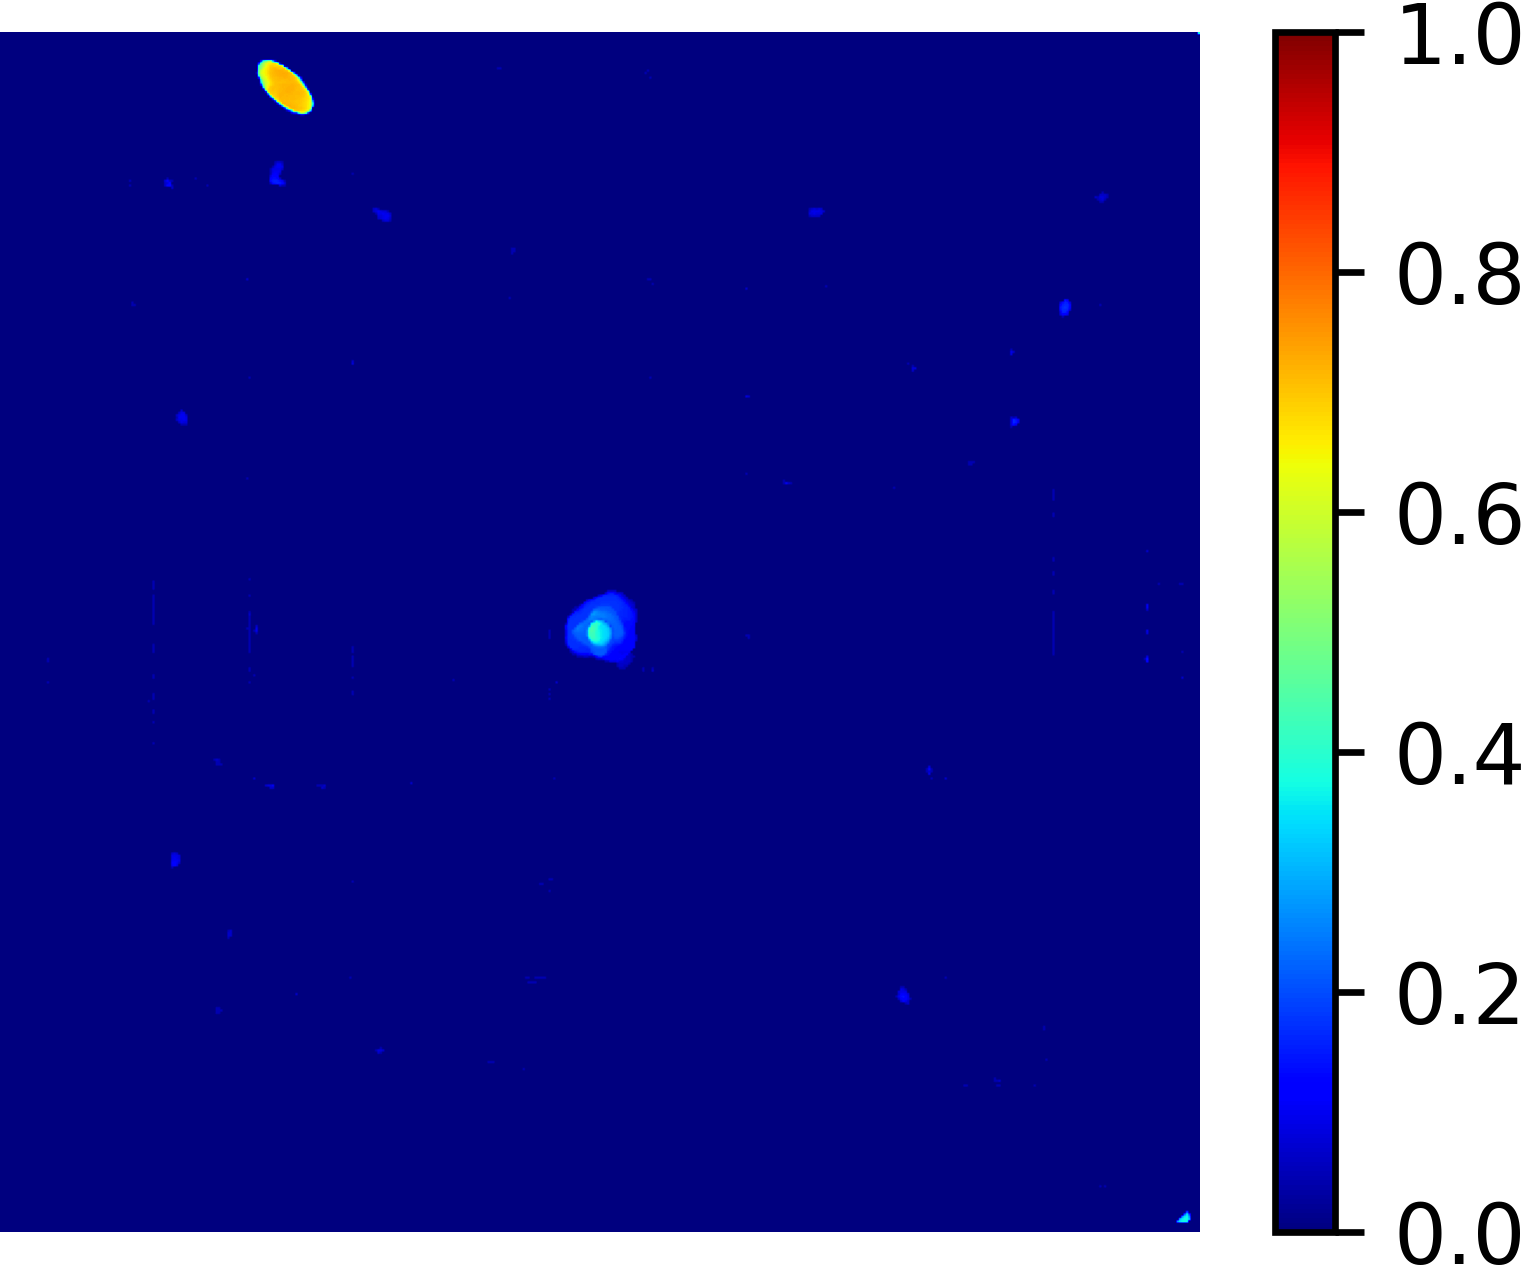
\includegraphics[height=3.05cm,keepaspectratio]{figures/RMS_Ijjeh_num_case_394.png}}\quad
				\subfloat[Binary RMS, IoU= 0.8]{
\includegraphics[height=3cm,keepaspectratio]{figures/Binary_RMS_Ijjeh_num_case394_.png}}
			\end{figure}
	\end{alertblock}}
\end{frame}
%%%%%%%%%%%%%%%%%%%%%%%%%%%%%%%%%%%%%%%%%%%%%%%%%%%%%%%%%%%%%%%%%%%%
\note{
	In the following three slides, I will present three numerical samples evaluated with the autoencoder ConvLSTM model.
	
	Animation (a) shows the full wavefield of 512 frames as an input to the model.
	Figure (b) shows the RMS damage map for all intermediate predictions,
	and figure (c) shows the binary RMS with IoU = 0.88.
	The second case is more complex, as the delamination is near the corner of the plate.
	In this case, the IoU is 0.58.
	The third case is also complex, as the delamination is located near the plate edge.
	In this case, the IoU is 0.8.		
}
%%%%%%%%%%%%%%%%%%%%%%%%%%%%%%%%%%%%%%%%%%%%%%%%%%%%%%%%%%%%%%%%%%%%
%	\begin{frame}{Animation based: Analysis of numerical cases}
	%		%%%%%%%%%%%%%%%%%%%%%%%%%%%%%%%%%%%%%%%%%%%%%%%%%%%%%%%%%%%%%%%%%%%%
	%		\begin{table}[!h]
		%			\centering
		%			\caption{Evaluation metrics of the three numerical cases.}
		%			\begin{tabular}{ccccc}
			%				\toprule[1.5pt]
			%				\multirow{2}{*}{case number} & \multicolumn{1}{c}{\multirow{2}{*}{A [mm\textsuperscript{2}]}} & \multicolumn{3}{c}{Predicted output} \\ 
			%				\cmidrule(lr){3-5} & & \multicolumn{1}{c}{IoU} & \multicolumn{1}{c}{\(\hat{A}\) [mm\textsuperscript{2}]} & \(\epsilon\) \\
			%				\midrule
			%				1 & 763 & \multicolumn{1}{c}{0.88} & \multicolumn{1}{c}{735} & \(3.67\%\) \\ 
			%				2 & 388 & \multicolumn{1}{c}{0.58} & \multicolumn{1}{c}{248} & \(36.08\%\) \\ 
			%				3 & 297 & \multicolumn{1}{c}{0.80} & \multicolumn{1}{c}{280} & \(5.72\%\) \\			 					
			%				\bottomrule[1.5pt]
			%			\end{tabular}	
		%			\label{tab:num_cases}
		%		\end{table}			
	%	\end{frame}
%	%%%%%%%%%%%%%%%%%%%%%%%%%%%%%%%%%%%%%%%%%%%%%%%%%%%%%%%%%%%%%%%%%%%%%%%%%%%%
%	\note{
	%		 The shown table presents the evaluation metrics for the autoencoder ConvLSTM model regarding the three numerical cases shown in the previous slide.
	%		 
	%		 The table gathers the actual delamination area, predicted delamination area, intersection over union IoU, and percentage area error \(\epsilon\) to each case.
	%	}
%%%%%%%%%%%%%%%%%%%%%%%%%%%%%%%%%%%%%%%%%%%%%%%%%%%%%%%%%%%%%%%%%%%%
\subsection*{Evaluation: Experimental cases}	
\setcounter{subfigure}{0}		%%%%%%%%%%%%%%%%%%%%%%%%%%%%%%%%%%%%%%%%%%%%%%%%%%%%%%%%%%%%%%%%%%%%
\begin{frame}{Experimental results: RMS image-based (Single delamination)}
	\begin{columns}[T]
		\begin{column}[t]{.25\textwidth}
			\begin{figure}[ht!]
				\centering
				\captionsetup{justification=centering}
				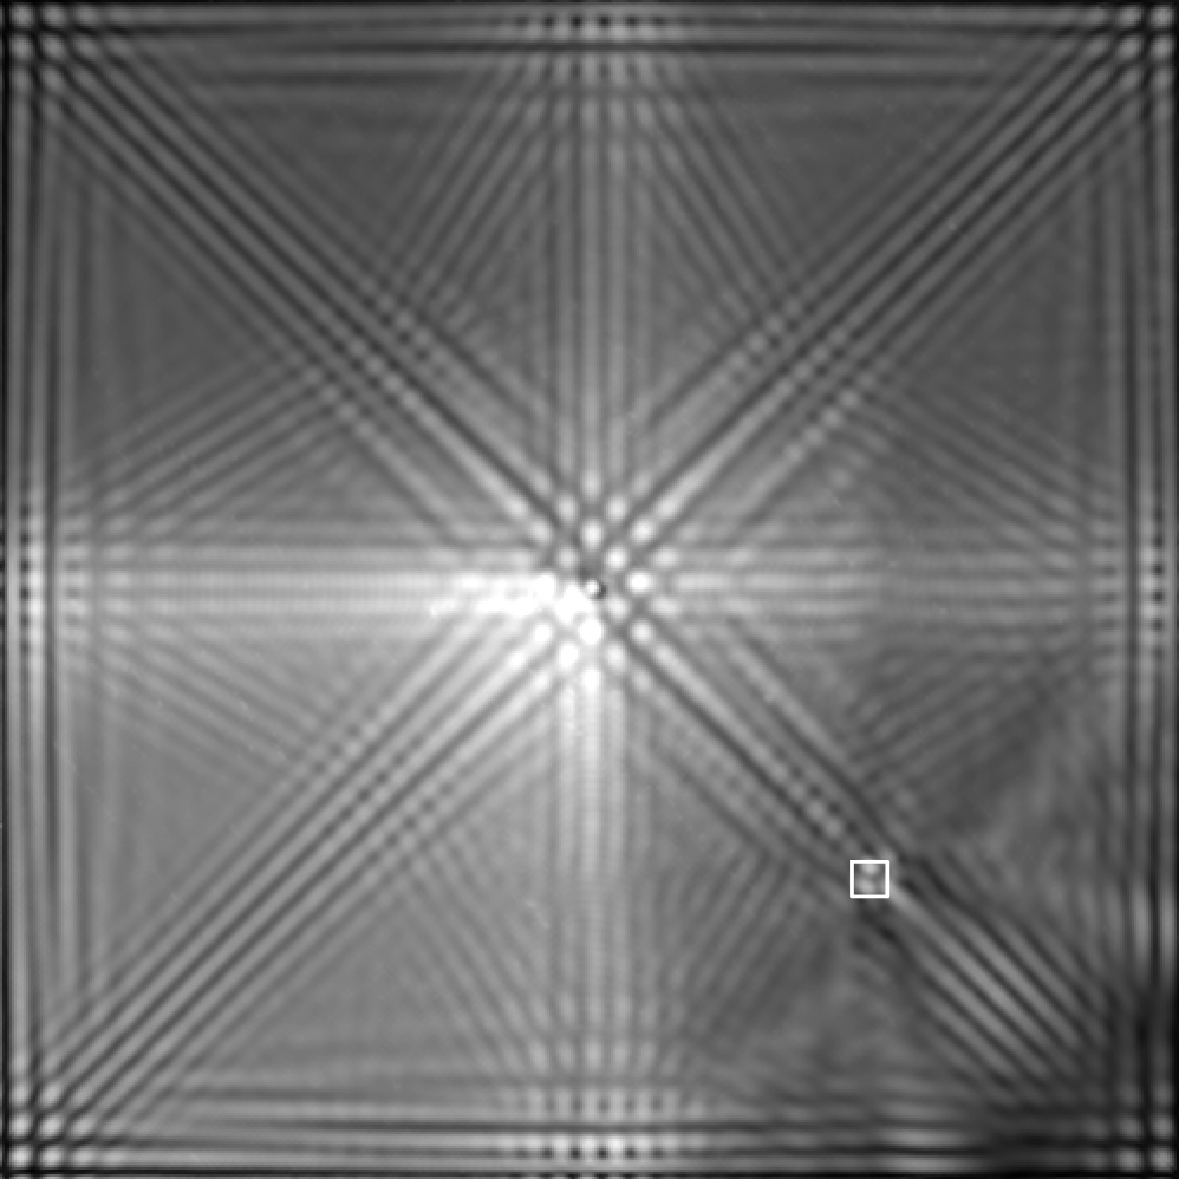
\includegraphics[height=.35\textheight]{ERMS_with_label.png}
				\caption{ERMS \& label}
			\end{figure}
			\justifying
			\tiny
			Kudela, P., Radzienski, M. and Ostachowicz, W., 2018. \textbf{Impact induced damage assessment by means of Lamb wave image processing}. \textit{Mechanical Systems and Signal Processing}, 102, pp.23-36.
		\end{column}
		\begin{column}[t]{0.5\textwidth}
			\begin{block}{Adaptive wavenumber filtering}
				\centering
				\footnotesize
				IoU=$0.401$
				\begin{figure}[ht!]
					\centering
					\captionsetup{justification=centering}
					\subfloat{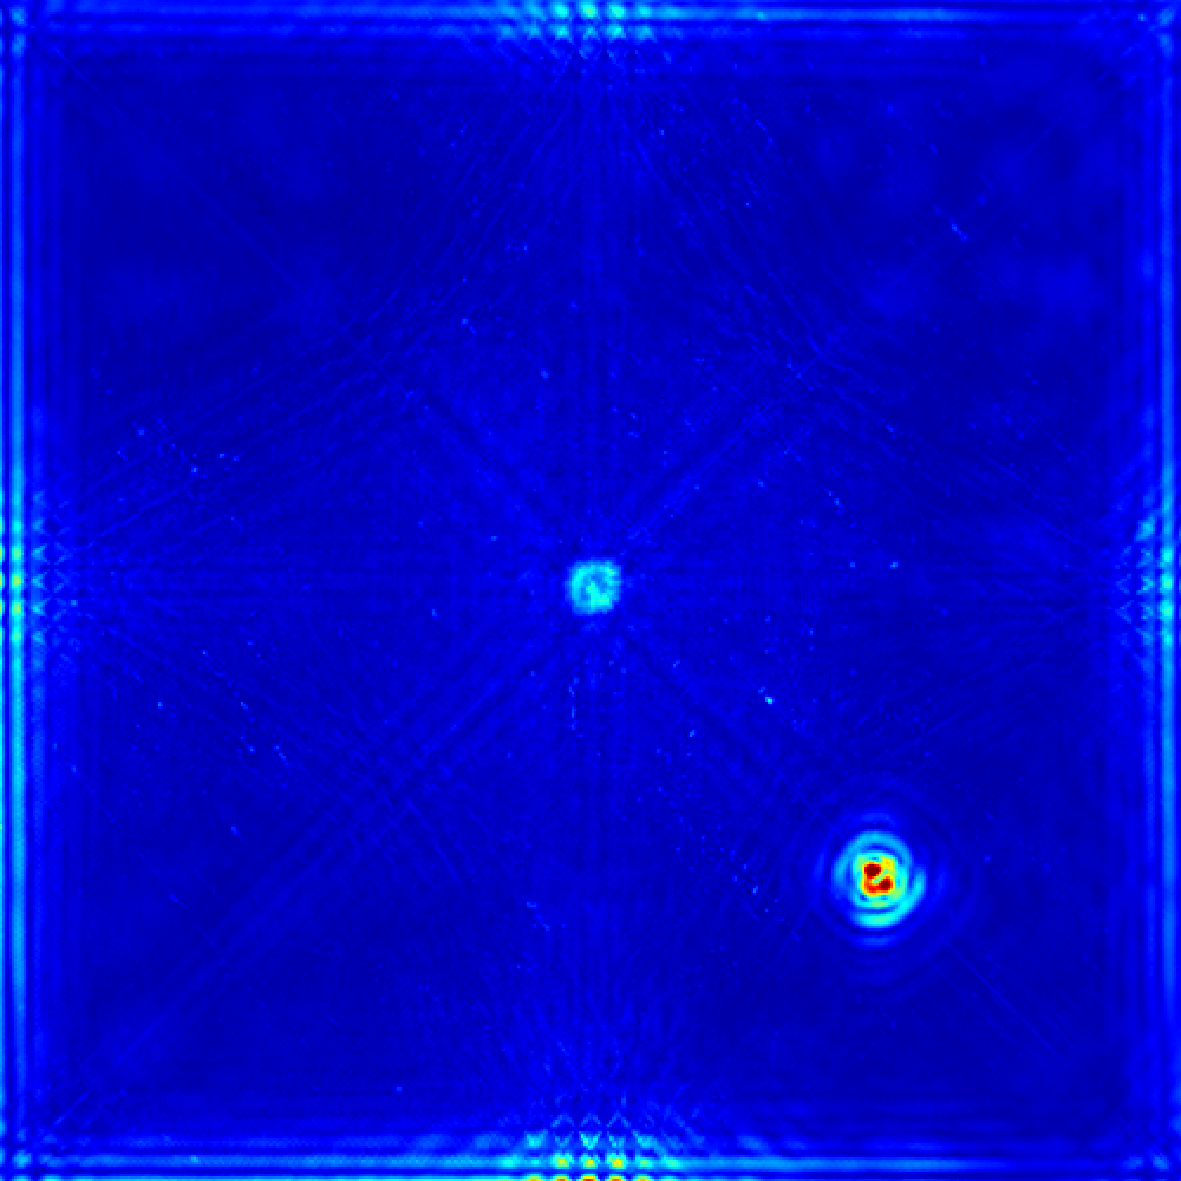
\includegraphics[height=.35\textheight]{ERMSF_CFRP_teflon_3o_375_375p_50kHz_5HC_x12_15Vpp.png}}
					\quad
					\subfloat{
\includegraphics[height=.35\textheight]{Binary_ERMSF_CFRP_teflon_3o_375_375p_50kHz_5HC_x12_15Vpp.png}}
				\end{figure}
			\end{block}					
		\end{column}		
		\begin{column}[t]{0.25\textwidth}
			\begin{alertblock}{DL approach: GCN}
				\centering
				\footnotesize
				IoU\(=0.723\)
				\begin{figure}[ht!]	
					\centering				
					\subfloat{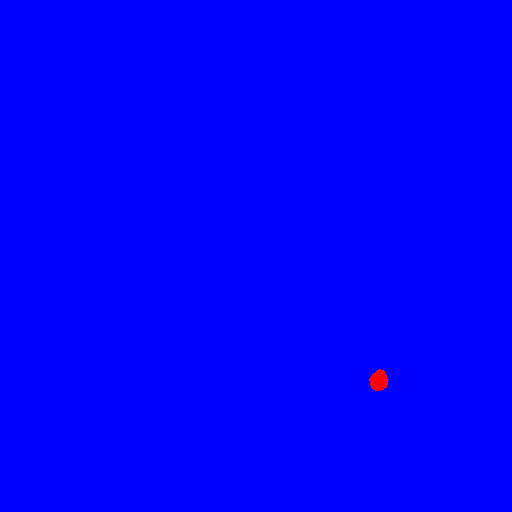
\includegraphics[height=.35\textheight]{Fig_GCN_7.png}}
				\end{figure} 	
			\end{alertblock}				
		\end{column}
	\end{columns}	
\end{frame}
%%%%%%%%%%%%%%%%%%%%%%%%%%%%%%%%%%%%%%%%%%%%%%%%%%%%%%%%%%%%%%%%%%%%
\note{
	In this slide, I present the experimental results of a specimen with a single delamination using the RMS-based model, the GCN.
	Additionally, I compared my developed model with the adaptive wavenumber filtering technique for damage imaging, which is a conventional signal processing technique.
	Figure (a) shows the ERMS with a label depicting the delamination. 
	Figure (b) shows the result of applying the adaptive wavenumber filtering method, and Figure (c) shows its binary output with IoU=0.401.
	Figure (d) shows the predicted damage map by the GCN model with IoU = 0.723.
	As shown, the deep learning model surpasses the conventional signal processing approach.
}
%%%%%%%%%%%%%%%%%%%%%%%%%%%%%%%%%%%%%%%%%%%%%%%%%%%%%%%%%%%%%%%%%%%%
%	\setcounter{subfigure}{0}
%	\begin{frame}{RMS based: Analysis of experimental case}
	%		\begin{table}[!ht]
		%			\centering
		%			\caption{Evaluation metrics of the experimental case.}
		%			\label{tab:rms_exp_case}
		%			\begin{tabular}{lc}
			%				\toprule[1.5pt]
			%				Model & IoU	\\			
			%				\midrule
			%				Res-UNet & 0.58 \\ 
			%				VGG16 encoder-decoder & 0.62 \\ 
			%				FCN-DenseNet & 0.54 \\ 
			%				PSPNet & 0.49 \\ 
			%				GCN & 0.72\\ 
			%				\bottomrule[1.5pt]
			%			\end{tabular}		
		%		\end{table}
	%%			\begin{table}[!ht]
		%%				\centering
		%%				\caption{Evaluation metrics of the experimental case.}
		%%				\label{tab:rms_exp_case}
		%%				\begin{tabular}{l@{\ }cccc}
			%%					\toprule
			%%					\multicolumn{1}{l}{Model} & \multicolumn{1}{c}{A [mm\textsuperscript{2}]} & \multicolumn{3}{c}{Predicted output} \\ 
			%%					\cmidrule(lr){3-5} & & \multicolumn{1}{c}{IoU} & \multicolumn{1}{c}{\(\hat{A}\) [mm\textsuperscript{2}]} & \(\epsilon\) \\ \midrule
			%%					Res-UNet & \multicolumn{1}{c}{\multirow{5}{*}{210}} & \multicolumn{1}{c}{0.58} & \multicolumn{1}{c}{323} & \(53.8\%\) \\ 
			%%					VGG16 encoder-decoder & & \multicolumn{1}{c}{0.62} & \multicolumn{1}{c}{320} & \(52.4\%\) 
			%%					\\ 
			%%					FCN-DenseNet & & \multicolumn{1}{c}{0.54} & \multicolumn{1}{c}{386} & \(83.8\%\) \\ 
			%%					PSPNet & & \multicolumn{1}{c}{0.49} & \multicolumn{1}{c}{580} & \(176.2\%\) 
			%%					\\ 
			%%					GCN & & \multicolumn{1}{c}{0.72} & \multicolumn{1}{c}{309} & \(47.1\%\) 
			%%					\\ 
			%%					\bottomrule
			%%				\end{tabular}		
		%%			\end{table}
	%	\end{frame}
%	%%%%%%%%%%%%%%%%%%%%%%%%%%%%%%%%%%%%%%%%%%%%%%%%%%%%%%%%%%%%%%%%%%%%
%	\note{
	%		The table shows the IoU values for all developed RMS based models for the single delamination specimen.
	%		
	%		Similarly to the numerical dataset, the best accuracy was achieved by using GCN.
	%		
	%%		As shown, the models are capable of precise detection and localisation of the delamination. 
	%%		We can see that the models can identify the delamination with almost free noise indicating the models are capable of generalising and detecting the delamination on previously unseen data. 
	%	}
%%%%%%%%%%%%%%%%%%%%%%%%%%%%%%%%%%%%%%%%%%%%%%%%%%%%%%%%%%%%%%%%%%%%
\setcounter{subfigure}{0}
\begin{frame}{Experimental results: Full wavefield based (Single delamination)}		
	\begin{alertblock}{DL approach}
		IoU= $0.41$% and $\epsilon=71.56\%$ 
		\begin{figure}[ht!]
			\centering
			\subfloat[Input]{\animategraphics[autoplay,loop,height=3cm]{16}{figures/gif_figs/CFRP_teflon_3o_375_375p_50kHz_5HC_x12_15Vpp/CFRP_teflon_30-}{1}{256}}\quad
			\subfloat[Intermidate ouputs]{\animategraphics[autoplay,loop,height=3cm]{15}{figures/gif_figs/CFRP_ijjeh_single_delamination/intermediate_output-}{0}{231}}\quad
			\subfloat[RMS]{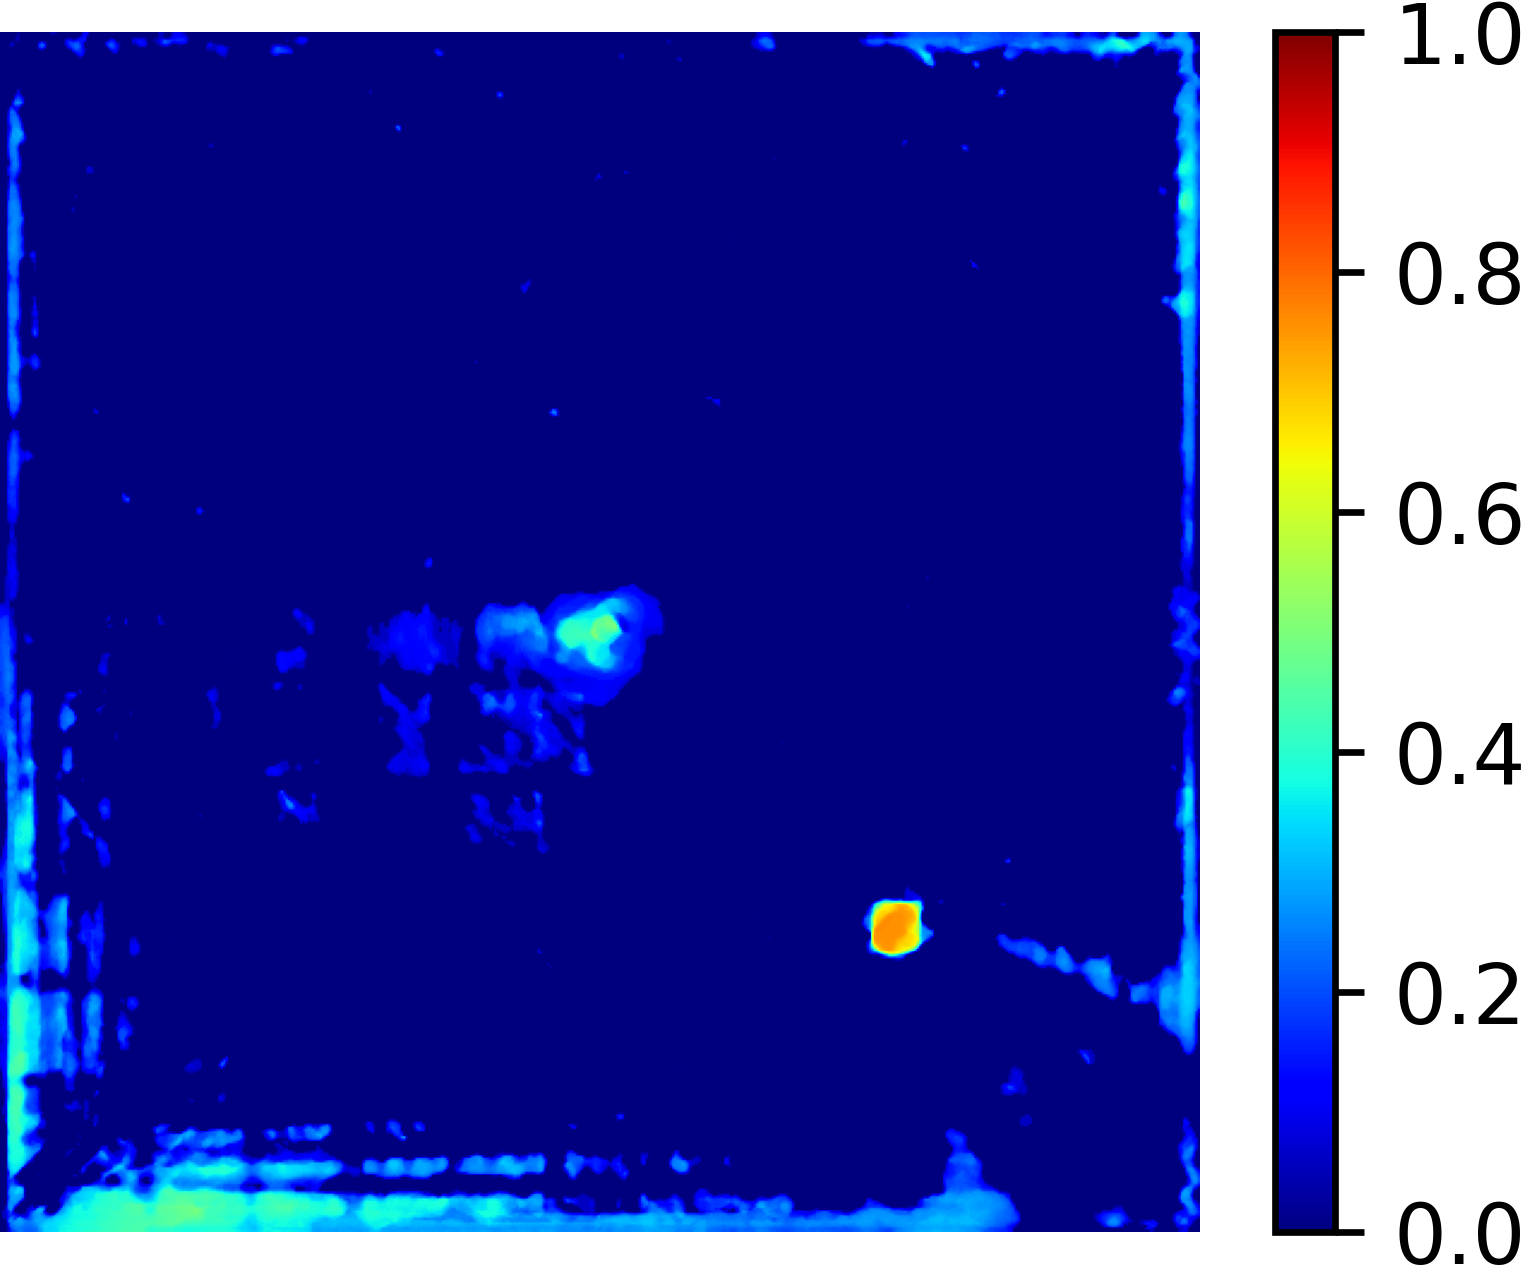
\includegraphics[height=3cm,keepaspectratio]{figures/RMS_CFRP_teflon_3o_375_375p_50kHz_5HC_x12_15Vpp_Ijjeh_updated_results_.png}}\quad
			\subfloat[Binary RMS]{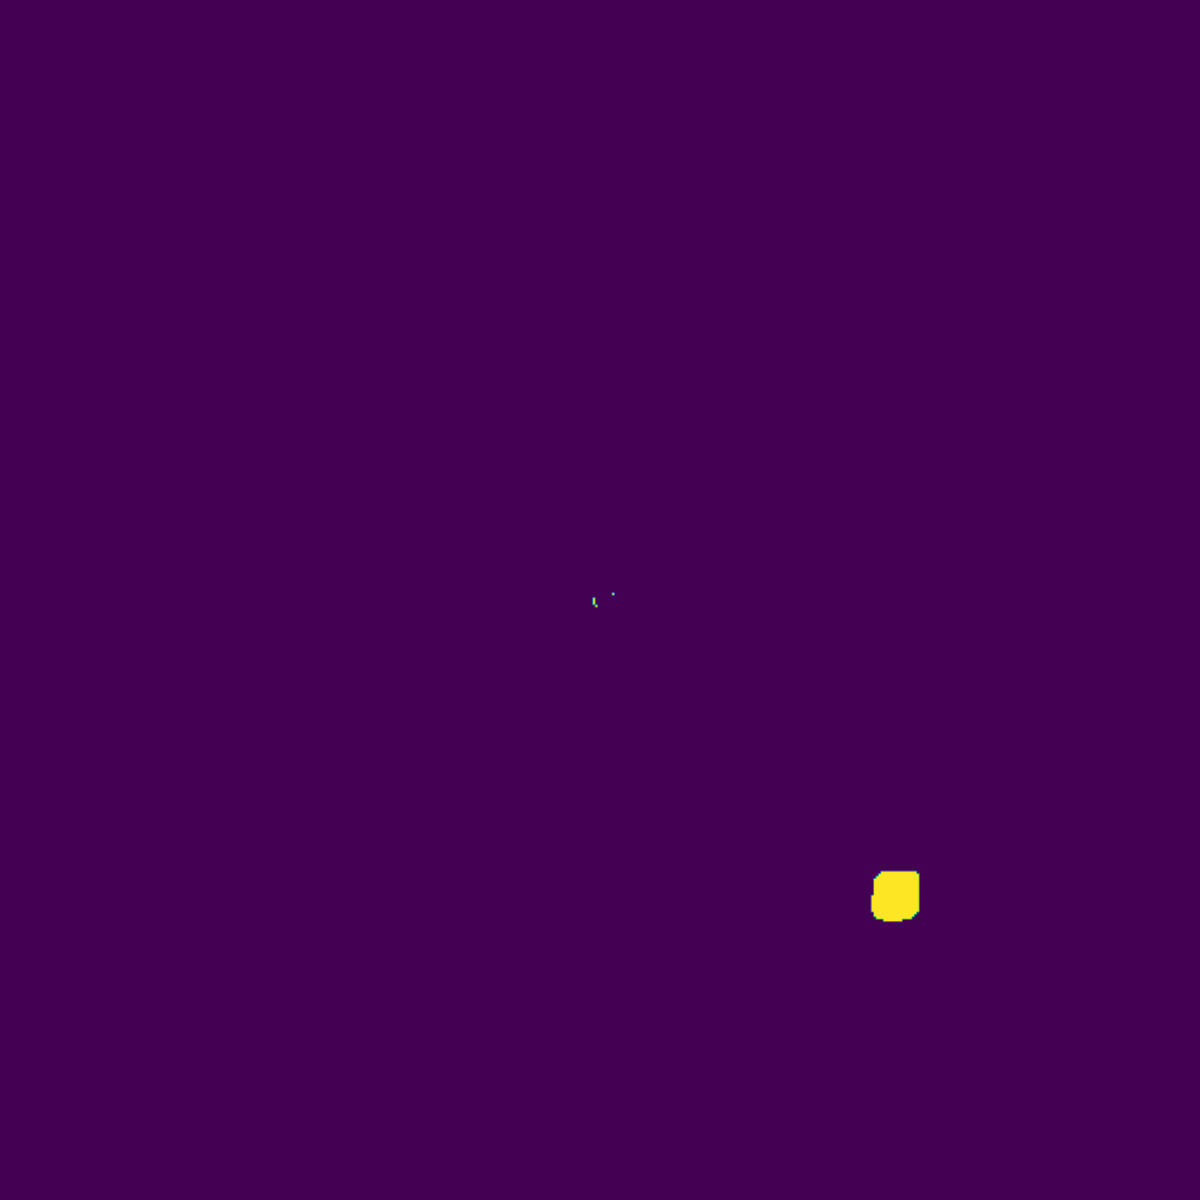
\includegraphics[height=3cm,keepaspectratio]{figures/Binary_RMS_CFRP_teflon_3o__375_375p_50kHz_5HC_x12_15Vpp_Ijjeh_.png}}
		\end{figure}			
	\end{alertblock}	
\end{frame}
%%%%%%%%%%%%%%%%%%%%%%%%%%%%%%%%%%%%%%%%%%%%%%%%%%%%%%%%%%%%%%%%%%%%
\note{
	In this slide, I present the predicted results using the autoencoder ConvLSTM model regarding the single delamination case.
	
	Animation (a) shows the full wavefield measured by SLDV with 256 frames.
	
	Animation (b) shows the intermediate predictions of the model. 
	
	Figure (c) shows the RMS of all intermediate predictions.
	
	And finally, Figure (d) shows the binary RMS with IoU= 0.41		
}
%%%%%%%%%%%%%%%%%%%%%%%%%%%%%%%%%%%%%%%%%%%%%%%%%%%%%%%%%%%%%%%%%%%%
\setcounter{subfigure}{0}	
\begin{frame}{Experimental results: Full wavefield based (Multiple delaminations)}
	\begin{columns}[T]
		\begin{column}[t]{0.20\textwidth}
			\begin{block}{Input}
				\footnotesize Full wavefield					
				\begin{figure}[ht!]	
					\centering						
					\subfloat{\animategraphics[autoplay,loop,height=0.32\textheight]{32}{figures/gif_figs/input_specimen_3/specimen_3-}{1}{512}}
				\end{figure}
			\end{block}				
		\end{column}
		\begin{column}[t]{0.40\textwidth}				
			\begin{block}{Adaptive wavenumber filtering}
				\footnotesize IoU$=0.04$					
				\begin{figure}[ht!]	
					\centering
					\subfloat{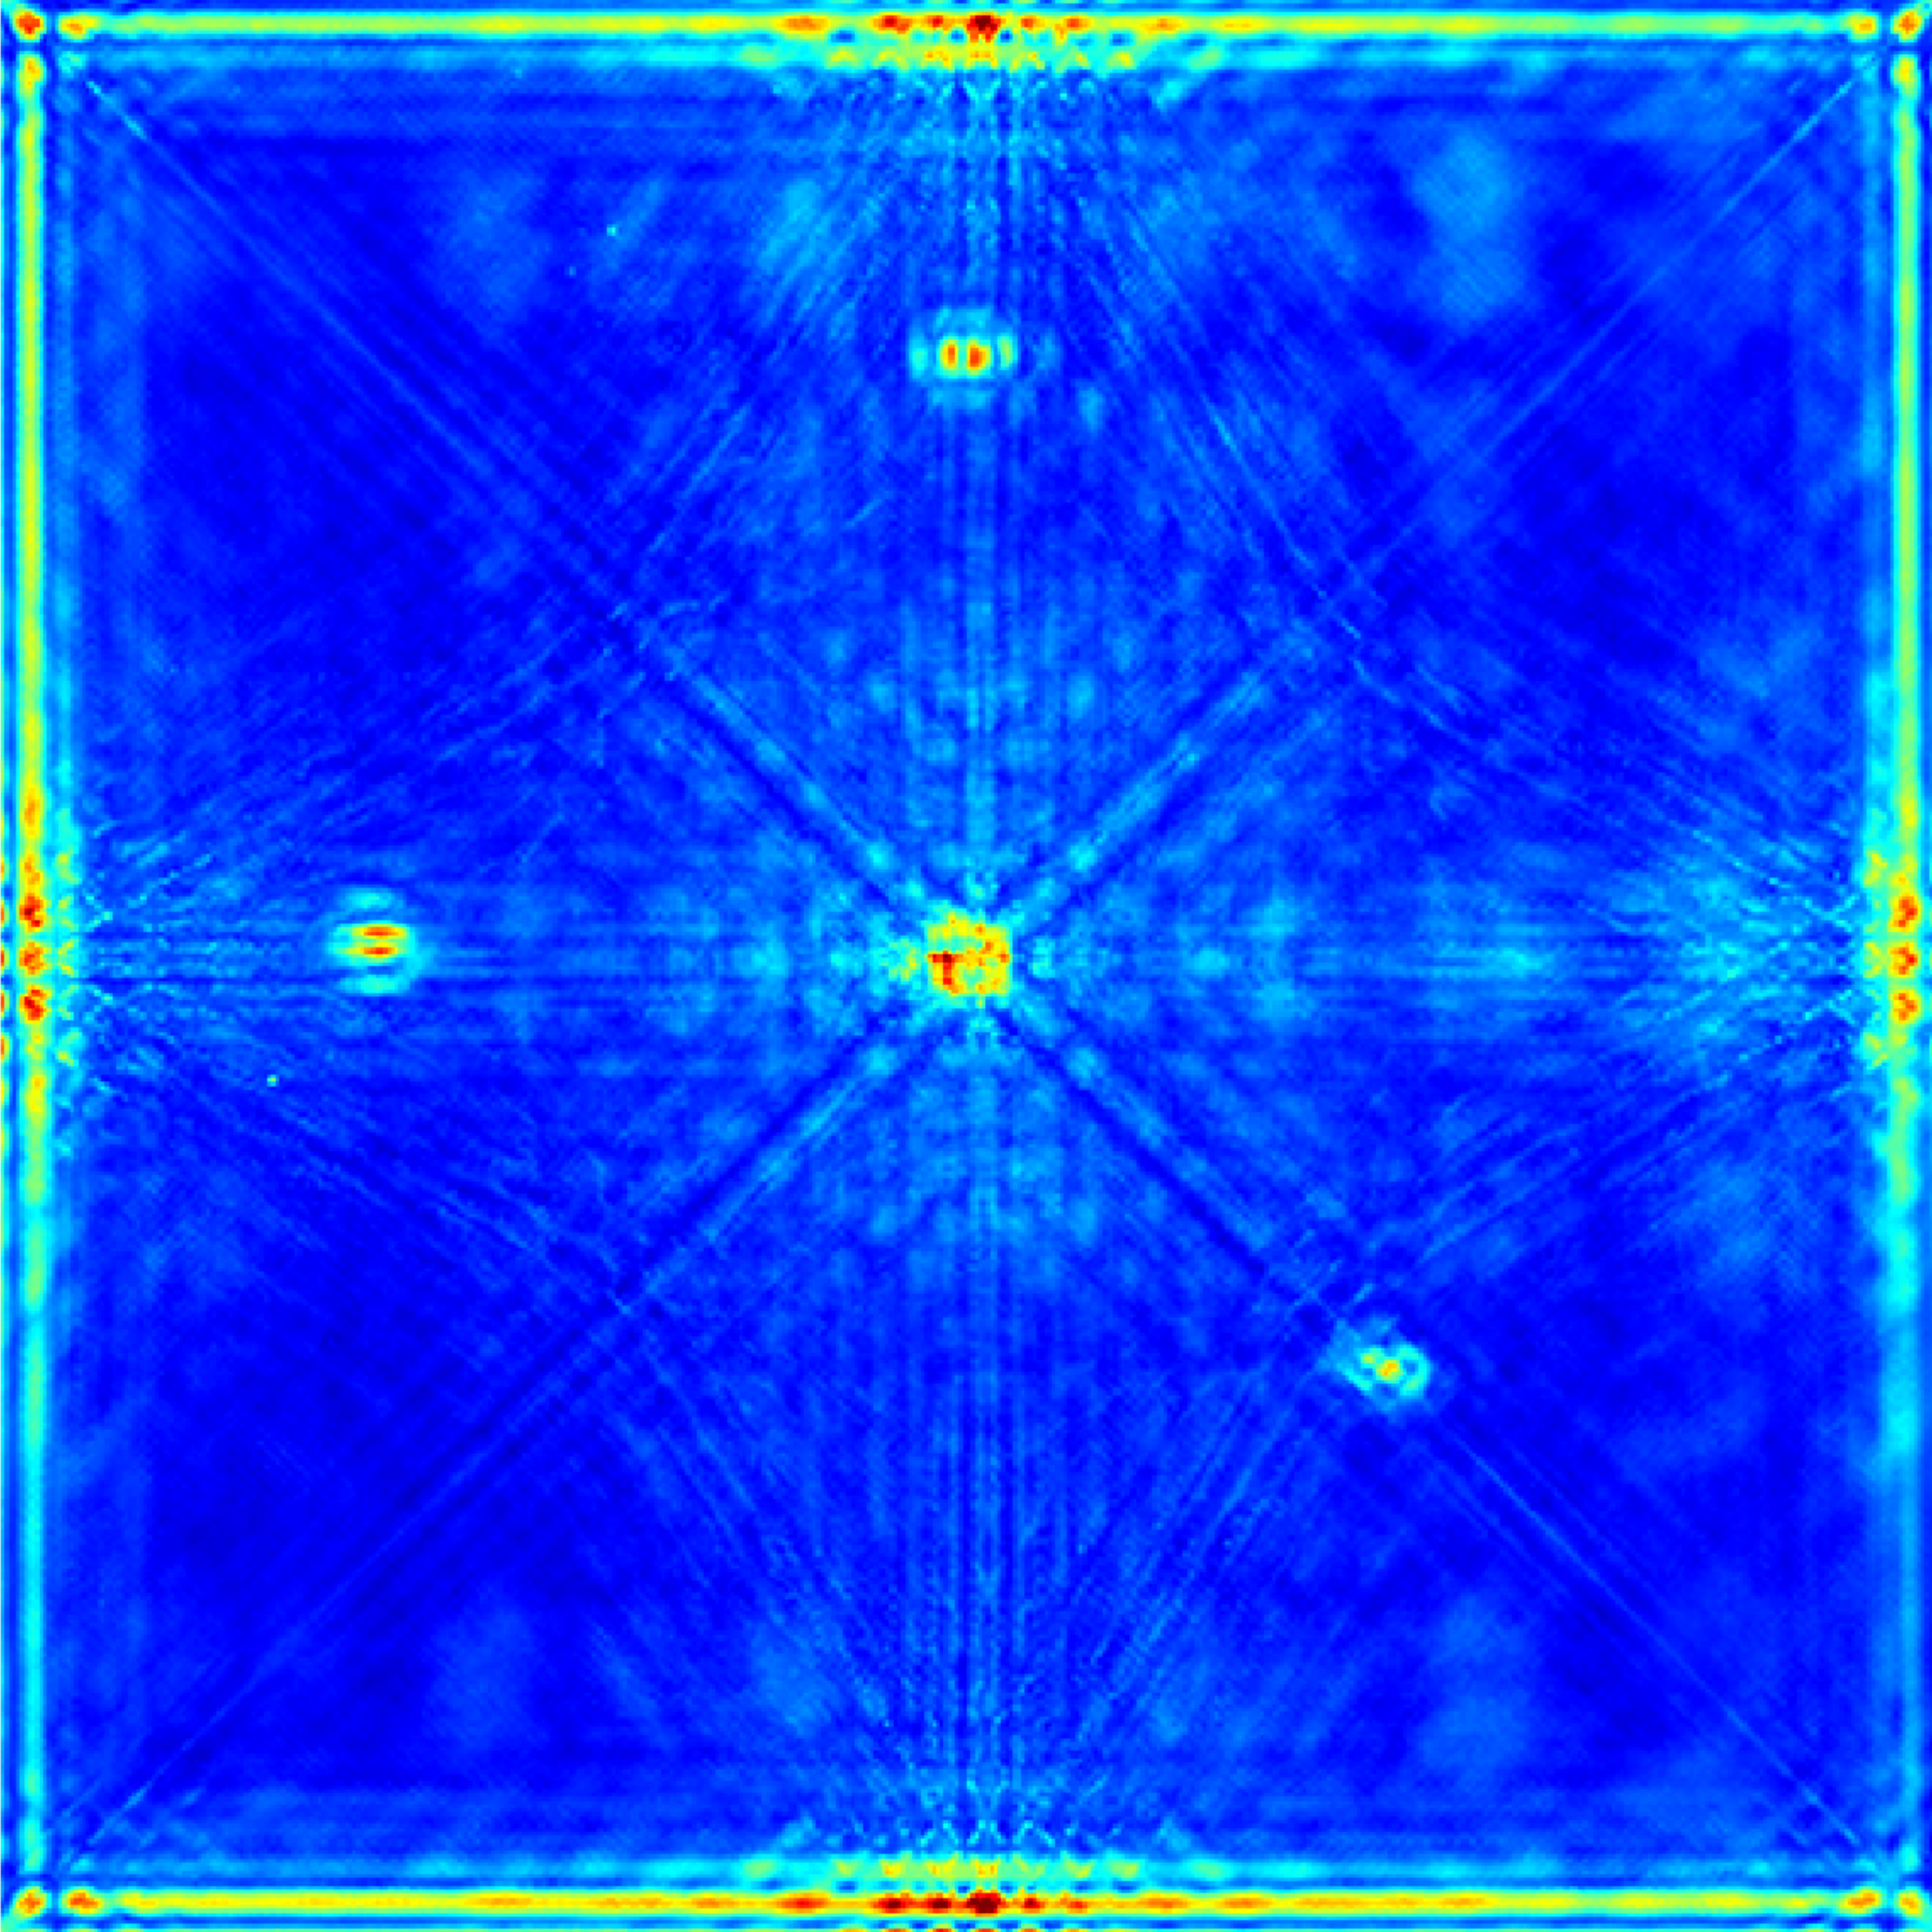
\includegraphics[height=0.32\textheight]{figures/mul/figure17a.png}}
					\quad
					\centering
					\subfloat{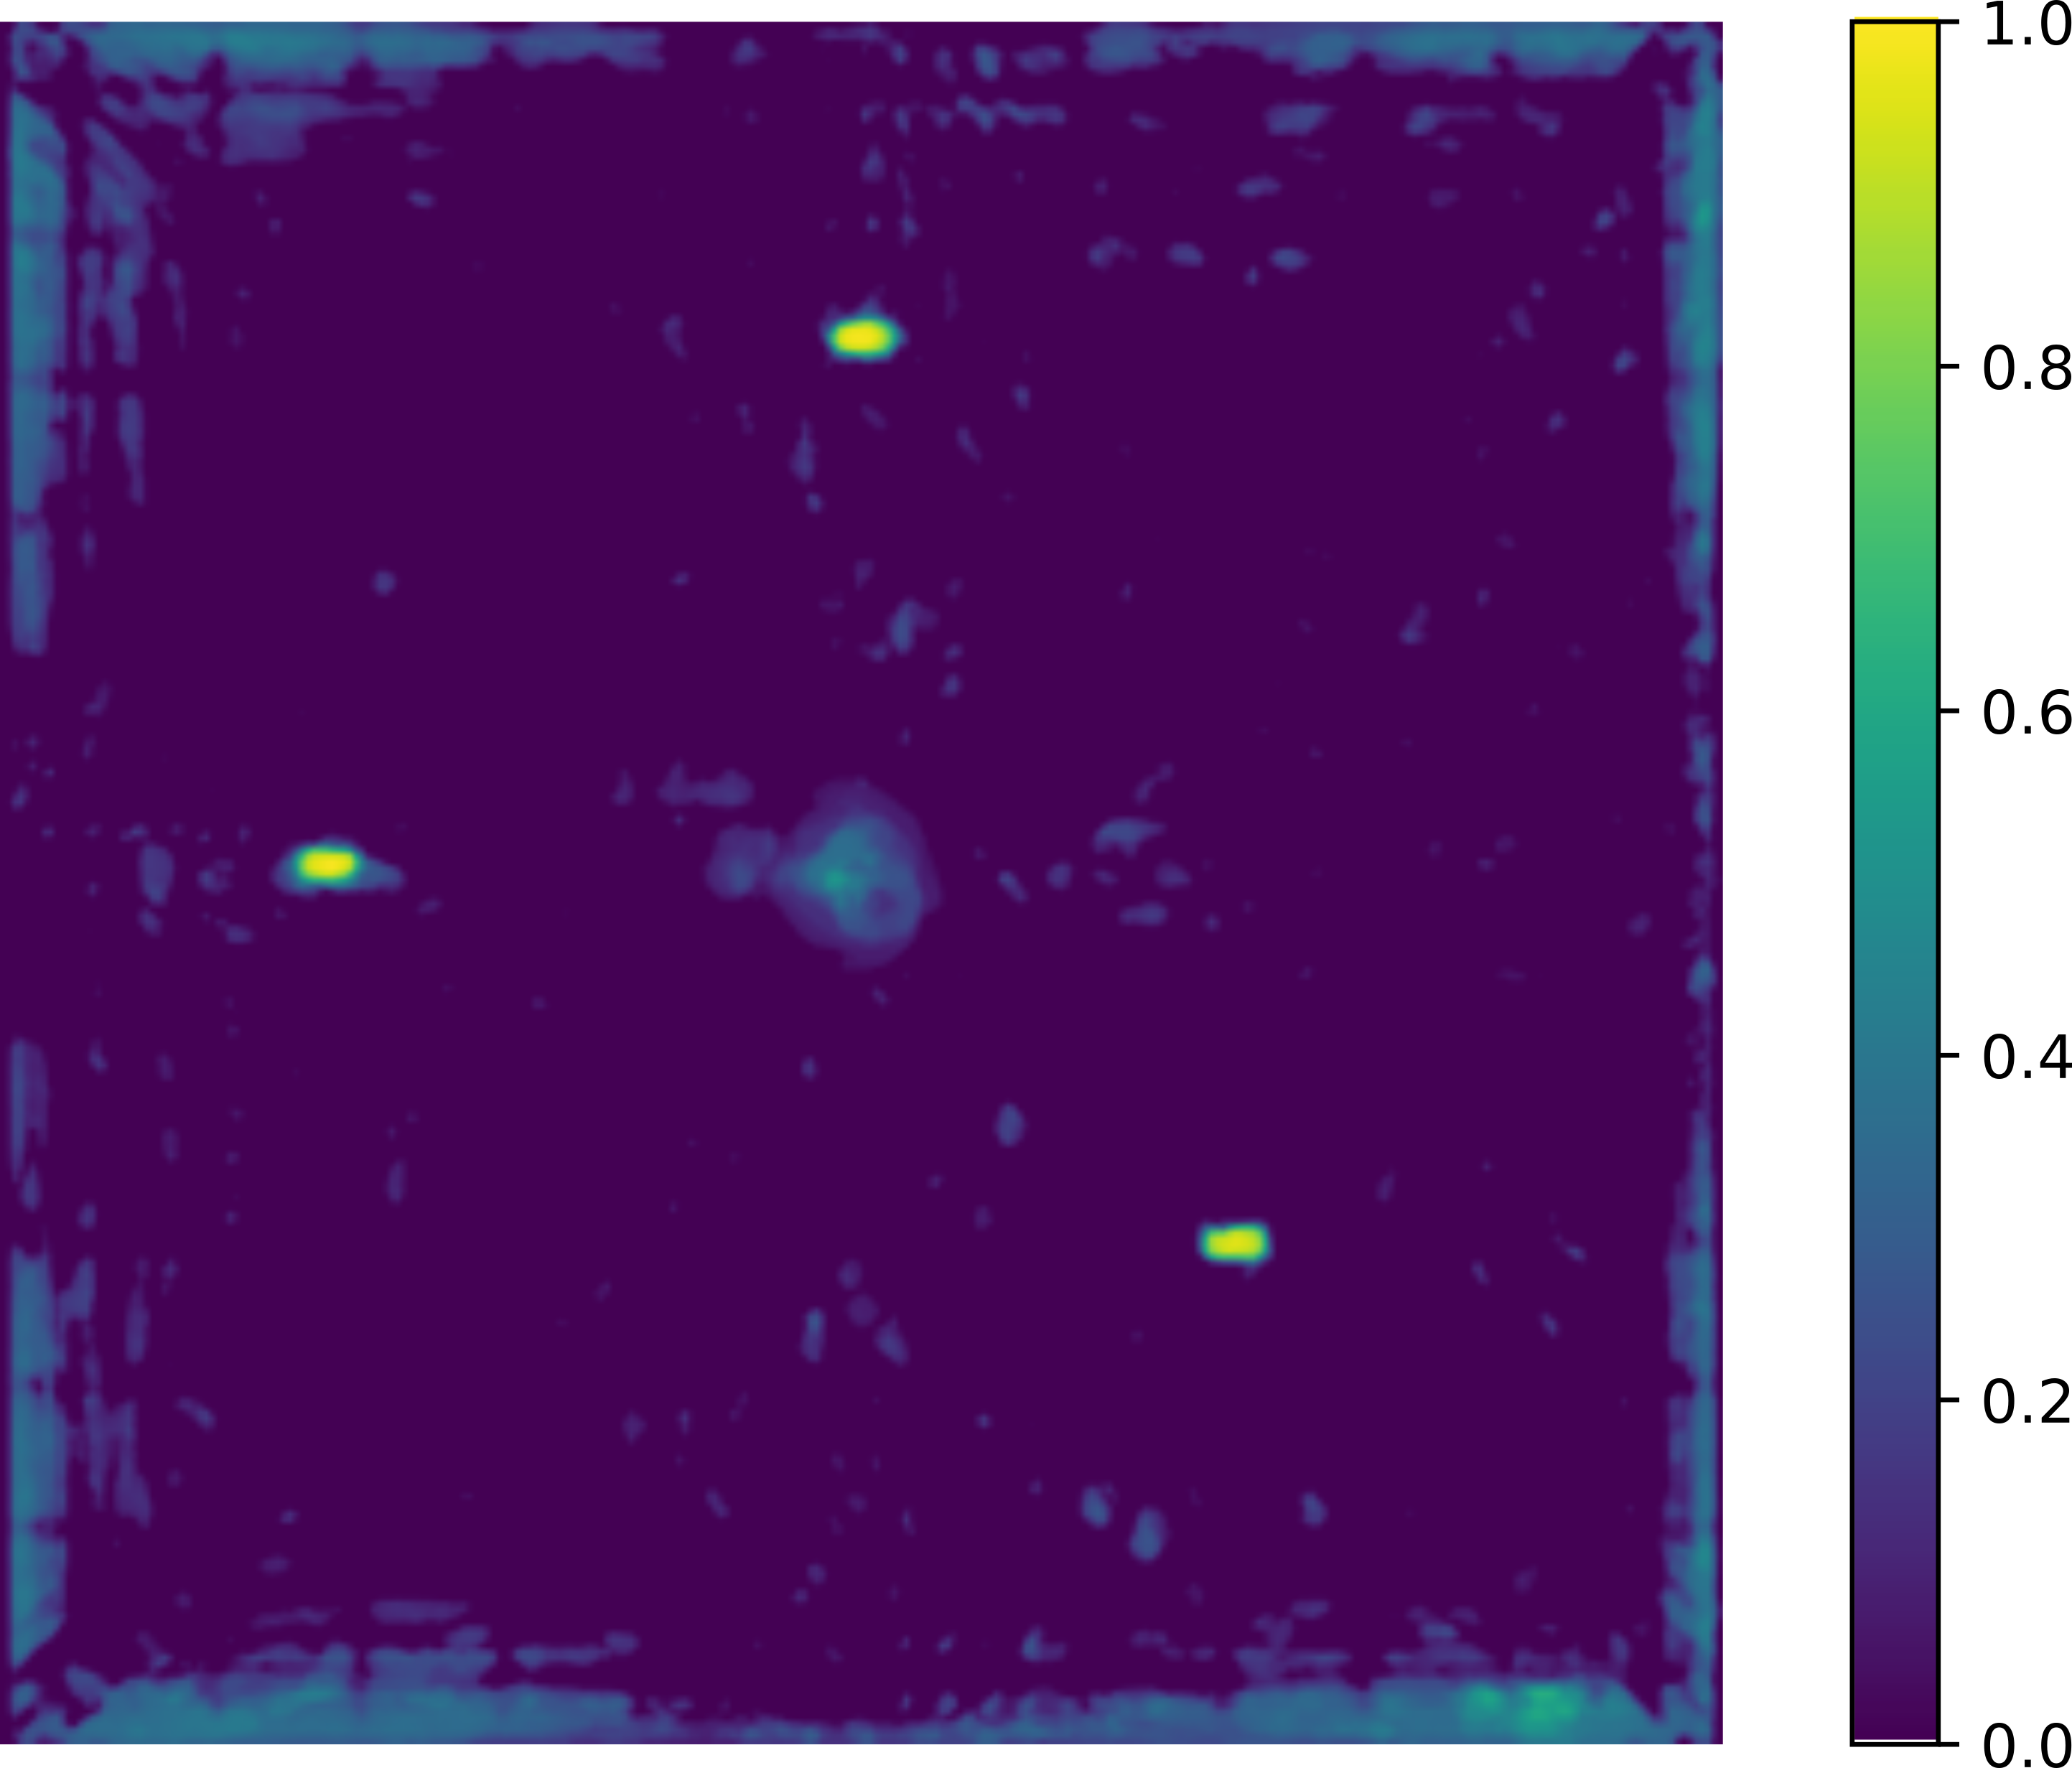
\includegraphics[height=0.32\textheight]{figures/mul/figure17b.png}}								
				\end{figure}
			\end{block}	
		\end{column}
		\begin{column}[t]{0.40\textwidth}				
			\begin{alertblock}{DL approach}	
				\footnotesize IoU= $0.64$						
				\begin{figure}[ht!]	
					\centering
					\subfloat{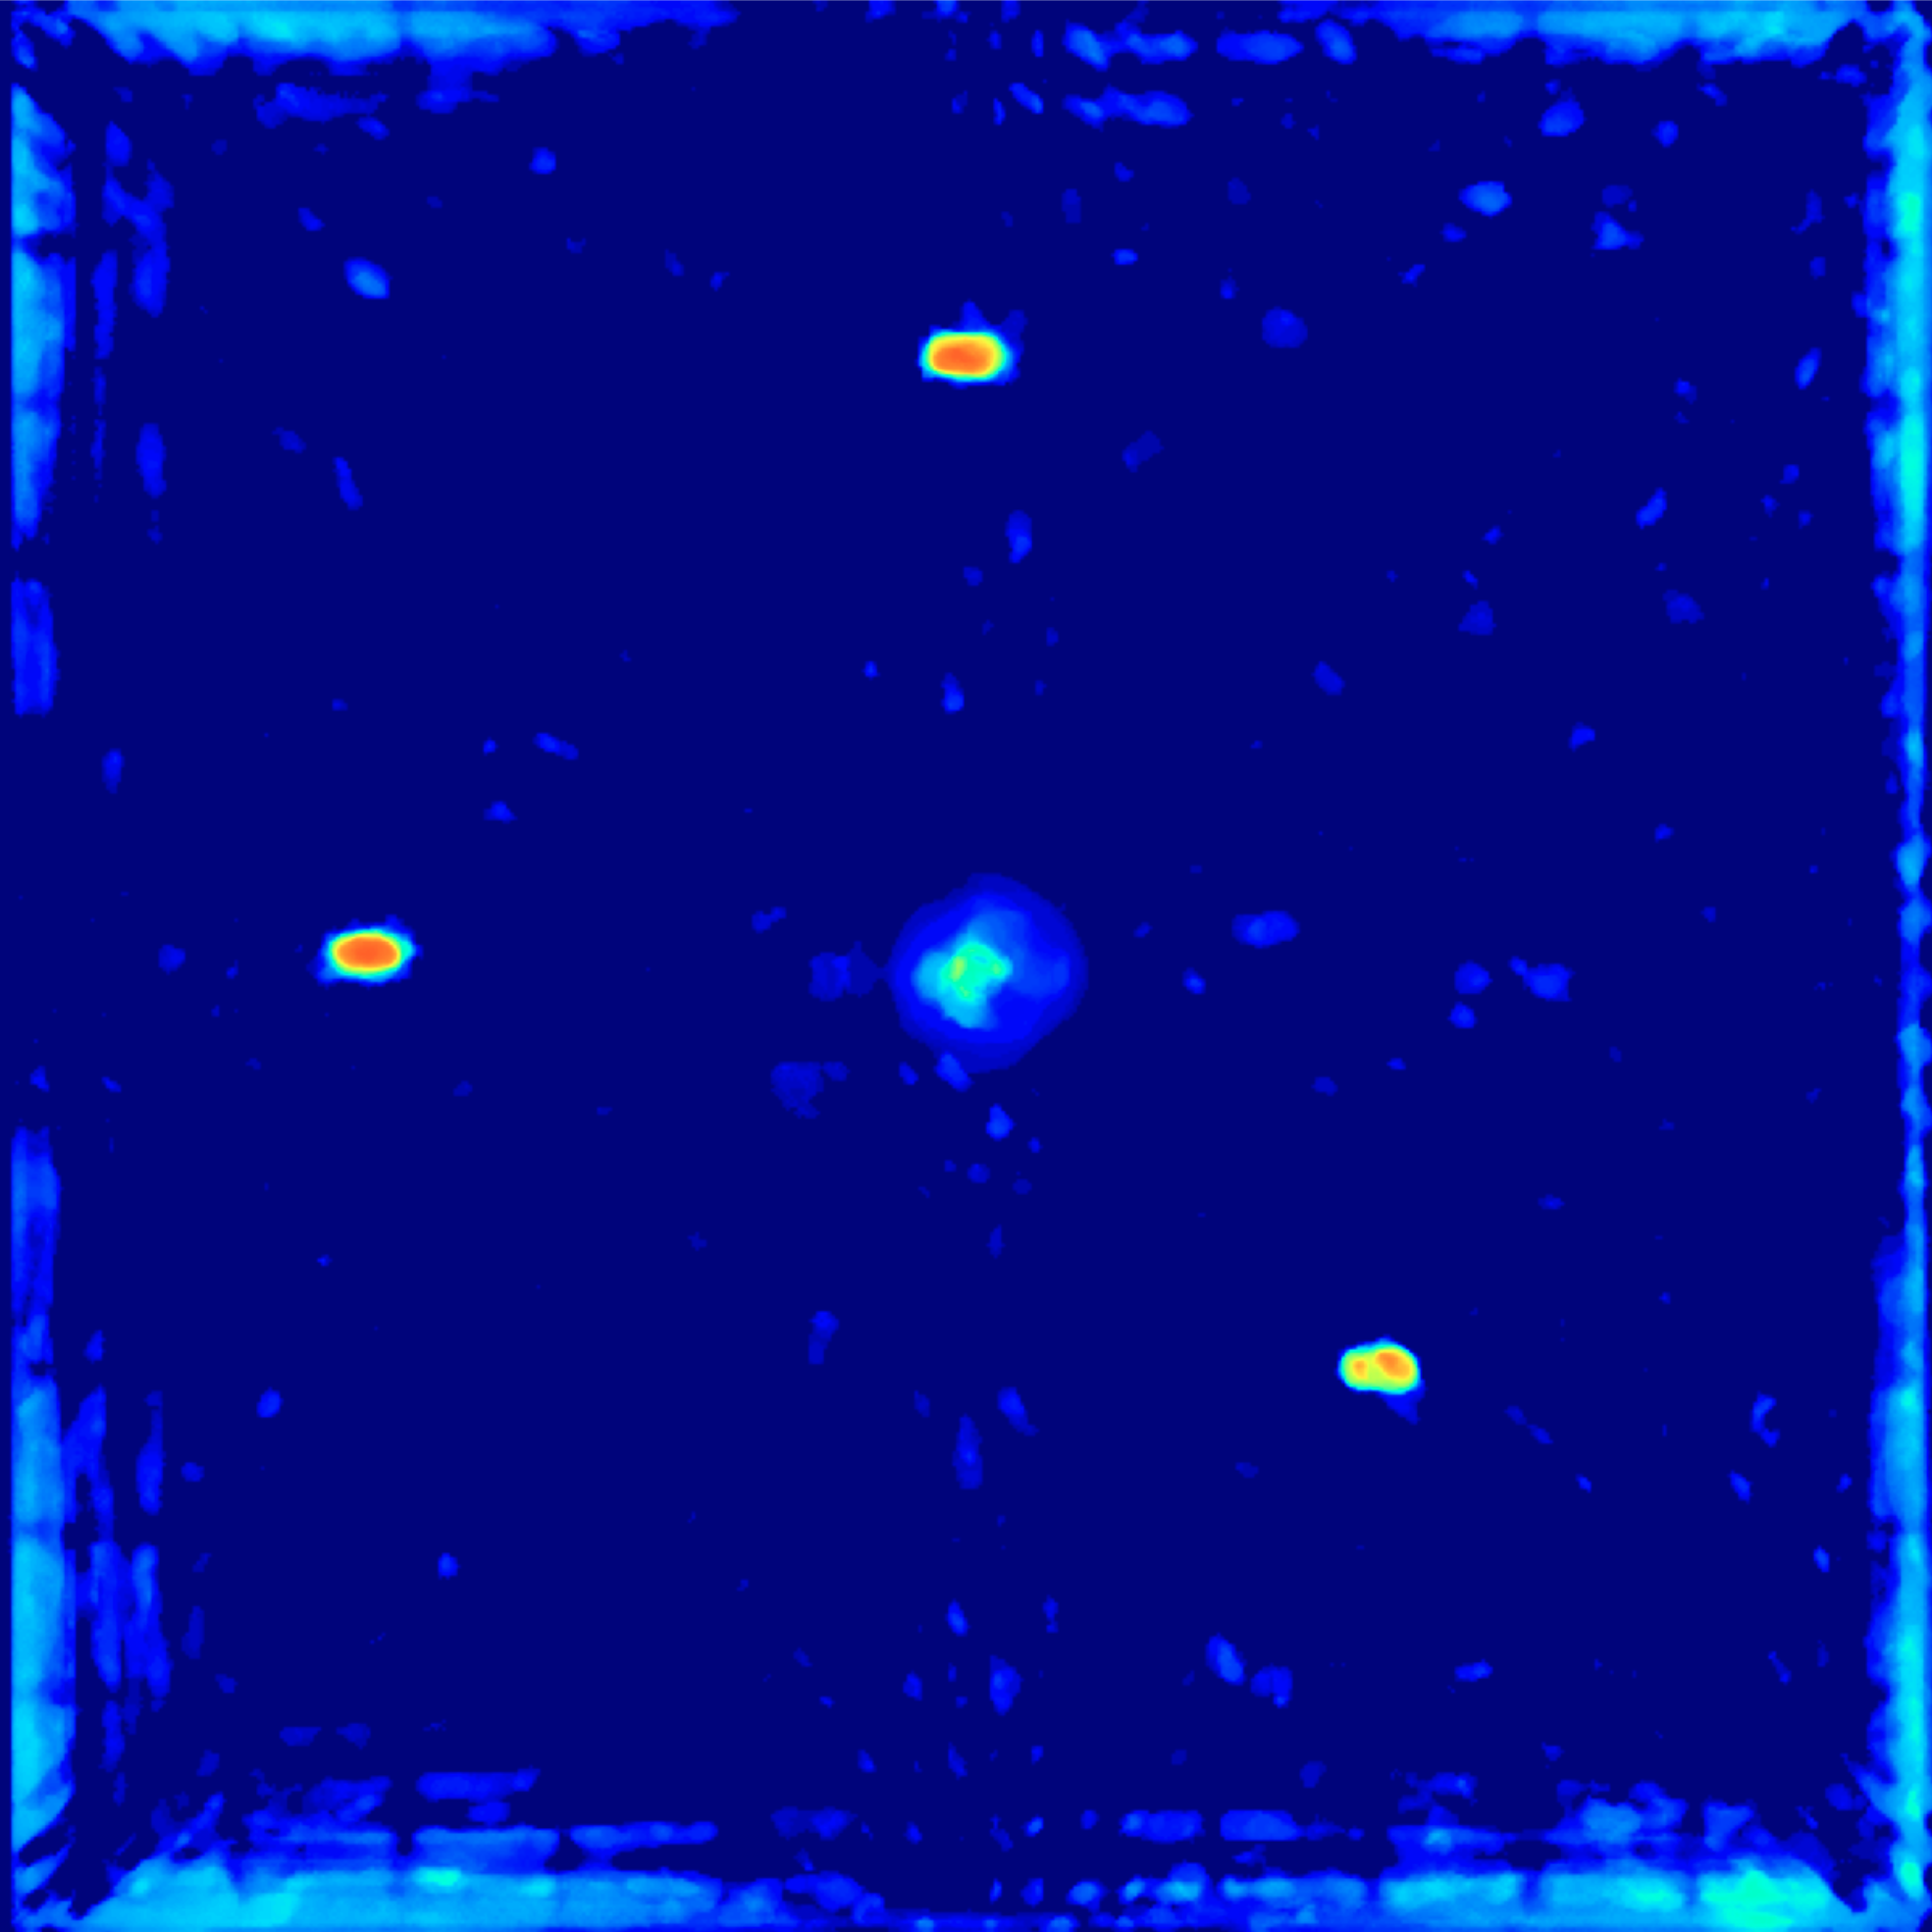
\includegraphics[height=0.32\textheight]{figures/RMS_L3_S3_B_333x333p_50kHz_5HC_18Vpp_x10_pzt_Ijjeh_updated_results_.png}}
					\quad
					\subfloat{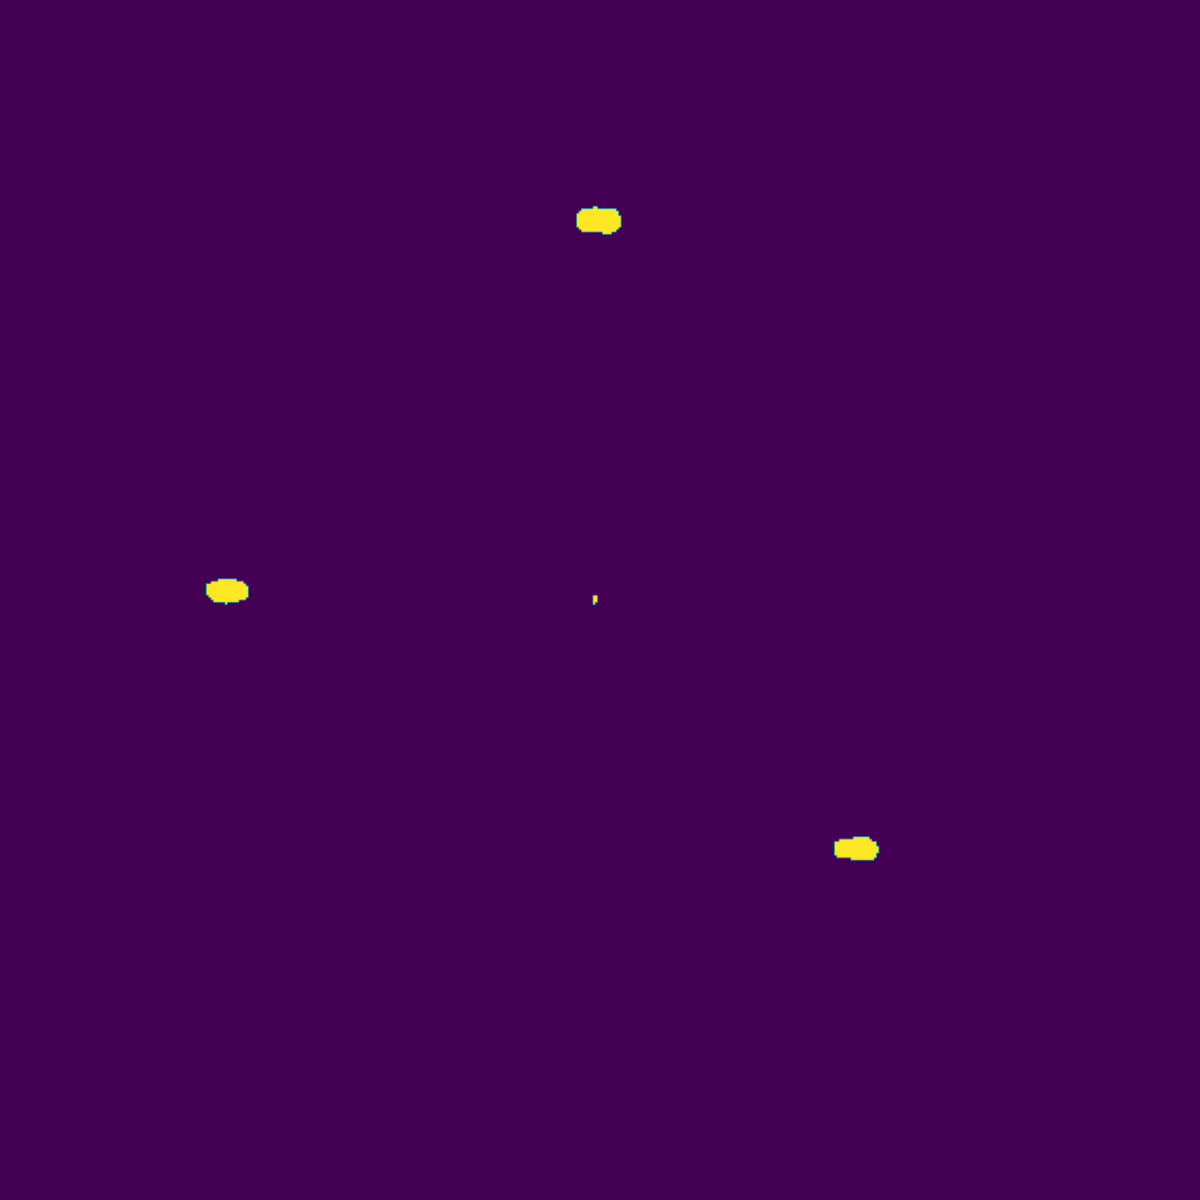
\includegraphics[height=0.32\textheight]{figures/Binary_RMS_L3_S3_B__333x333p_50kHz_5HC_18Vpp_x10_pzt_Ijjeh_.png}}						
				\end{figure}				
			\end{alertblock}				
		\end{column}				
	\end{columns}	
\end{frame}
%%%%%%%%%%%%%%%%%%%%%%%%%%%%%%%%%%%%%%%%%%%%%%%%%%%%%%%%%%%%%%%%%%%%
\note{
	Here, I present the predicted results using the autoencoder ConvLSTM model compared to adaptive wavenumber filtering for the multiple delamination case.
	The animation on the left shows the full wavefield measured by the SLDV of 512 frames.
	The figure shows the damage map resulting from applying adaptive wavenumber filtering, and this figure shows its binary output with IoU = 0.04
	Figure shows the RMS of all intermediate predictions, and figure shows the binary RMS with IoU = 0.64
	It can be concluded that utilising animations of Lamb waves propagation has better outcomes for delamination identification than the processing of a single image representing signal energy or RMS.		
}
%%%%%%%%%%%%%%%%%%%%%%%%%%%%%%%%%%%%%%%%%%%%%%%%%%%%%%%%%%%%%%%%%%%%
\setcounter{subfigure}{0}
%%%%%%%%%%%%%%%%%%%%%%%%%%%%%%%%%%%%%%%%%%%%%%%%%%%%%%%%%%%%%%%%%%%%
\subsection{Part II: Super-resolution image reconstruction}
\begin{frame}{Super-resolution image reconstruction}
	\begin{columns}[T]
		\begin{column}[t]{0.6\textwidth}
			\begin{alertblock}{Deep learning super-resolution model (DLSR)}					
				\begin{footnotesize}
					\justifying
					\settowidth{\leftmargini}{\usebeamertemplate{itemize item}}
					\addtolength{\leftmargini}{\labelsep}
					\begin{itemize}
						\item Registering HR full wavefield with an SLDV is a~time-consuming process.
						\item DLSR model aims to recover HR full wavefield scans from a~LR measurements (below the Nyquist-Shannon sampling rate).
					\end{itemize} 
				\end{footnotesize}					
			\end{alertblock}						
			\begin{exampleblock}{Compressive sensing (CS) theory}
				\footnotesize
				\justifying
				Any natural signal (\(x\)), e.g. (sounds, images) can be recovered using considerably fewer measurements (\(y\)) than standard methods.
				\vfill
				\begin{figure}[ht!]
					\centering
					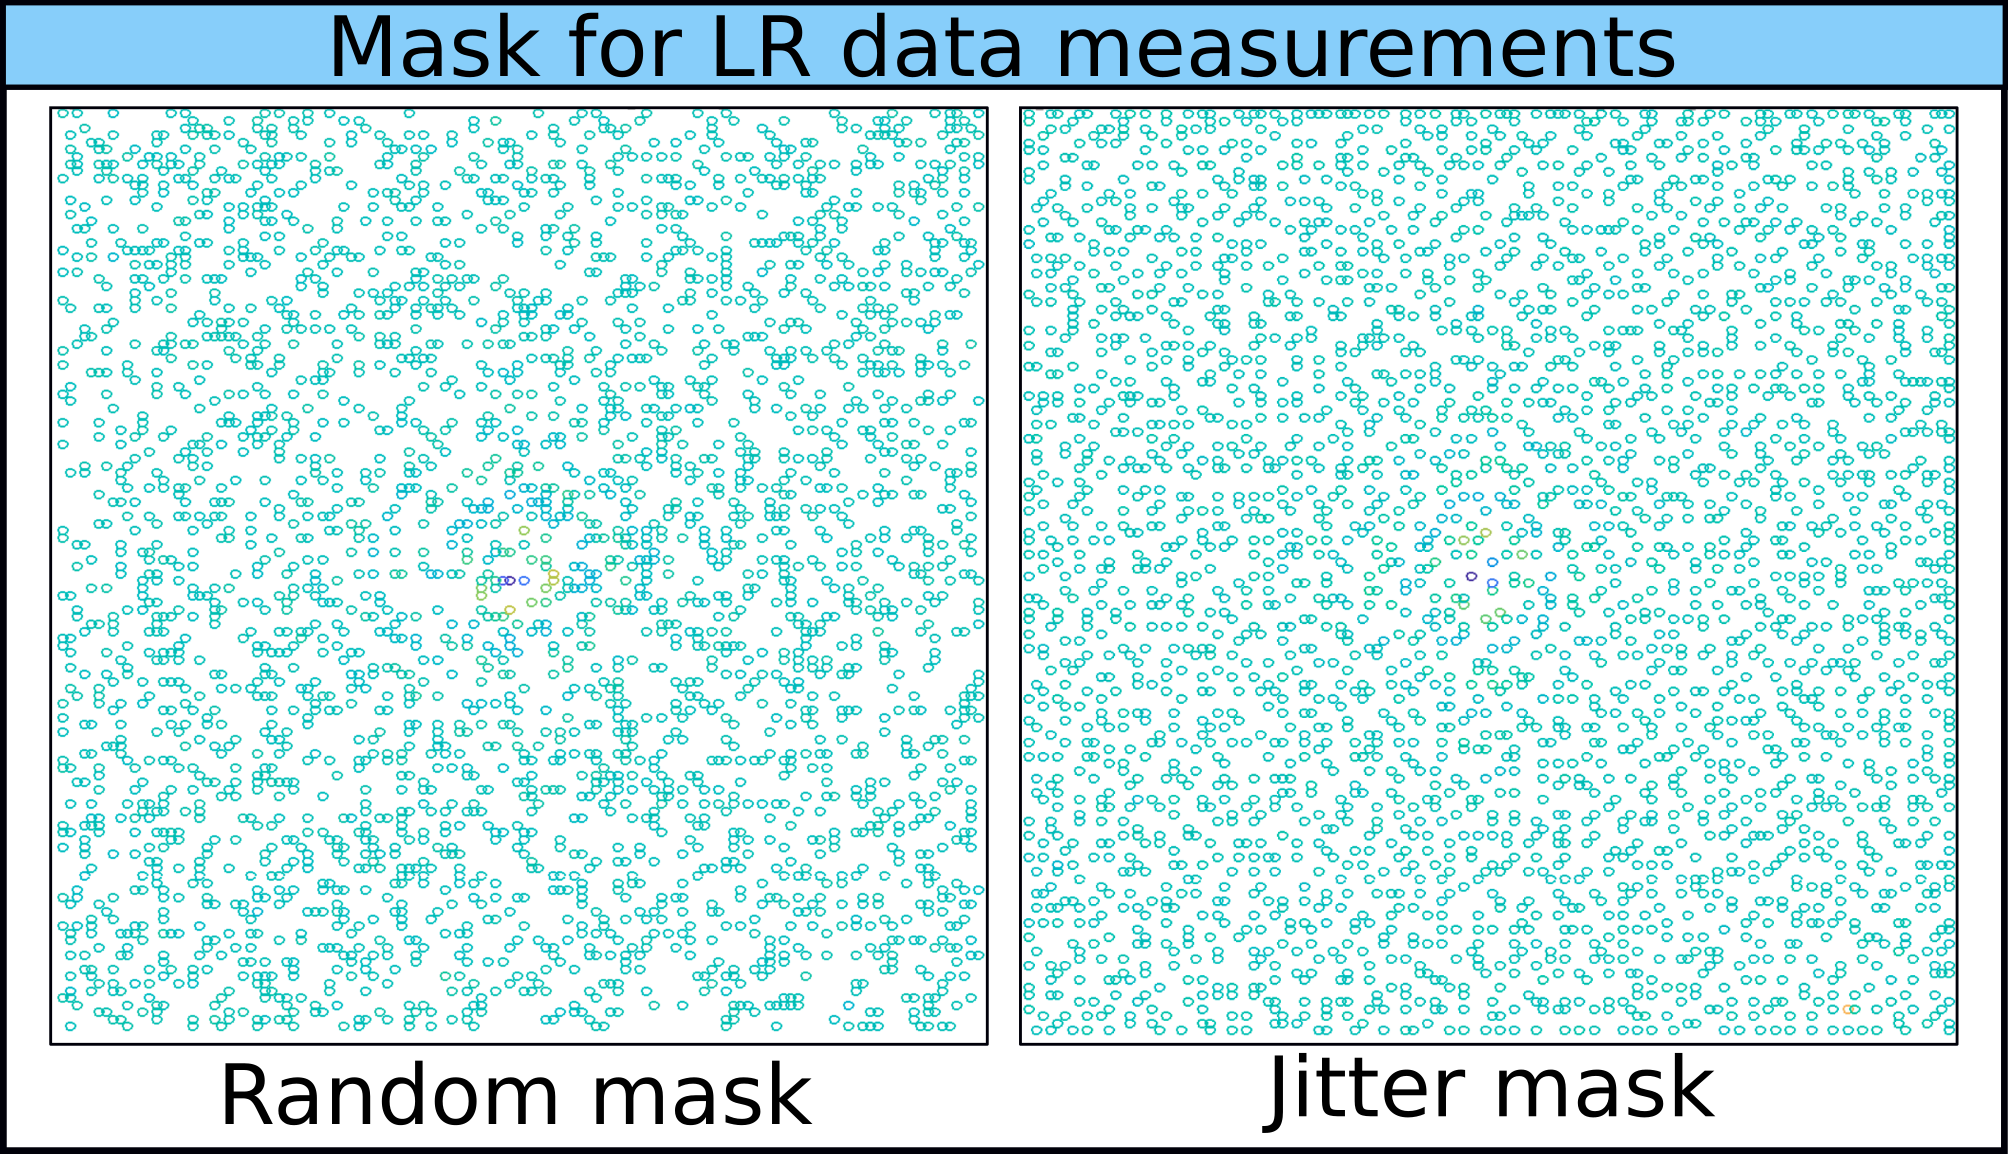
\includegraphics[width=.45\textwidth]{matrix_mask.png}
				\end{figure}
			\end{exampleblock}							
		\end{column}
		\begin{column}[t]{0.4\textwidth}
			\begin{figure}[ht!]
				\centering
				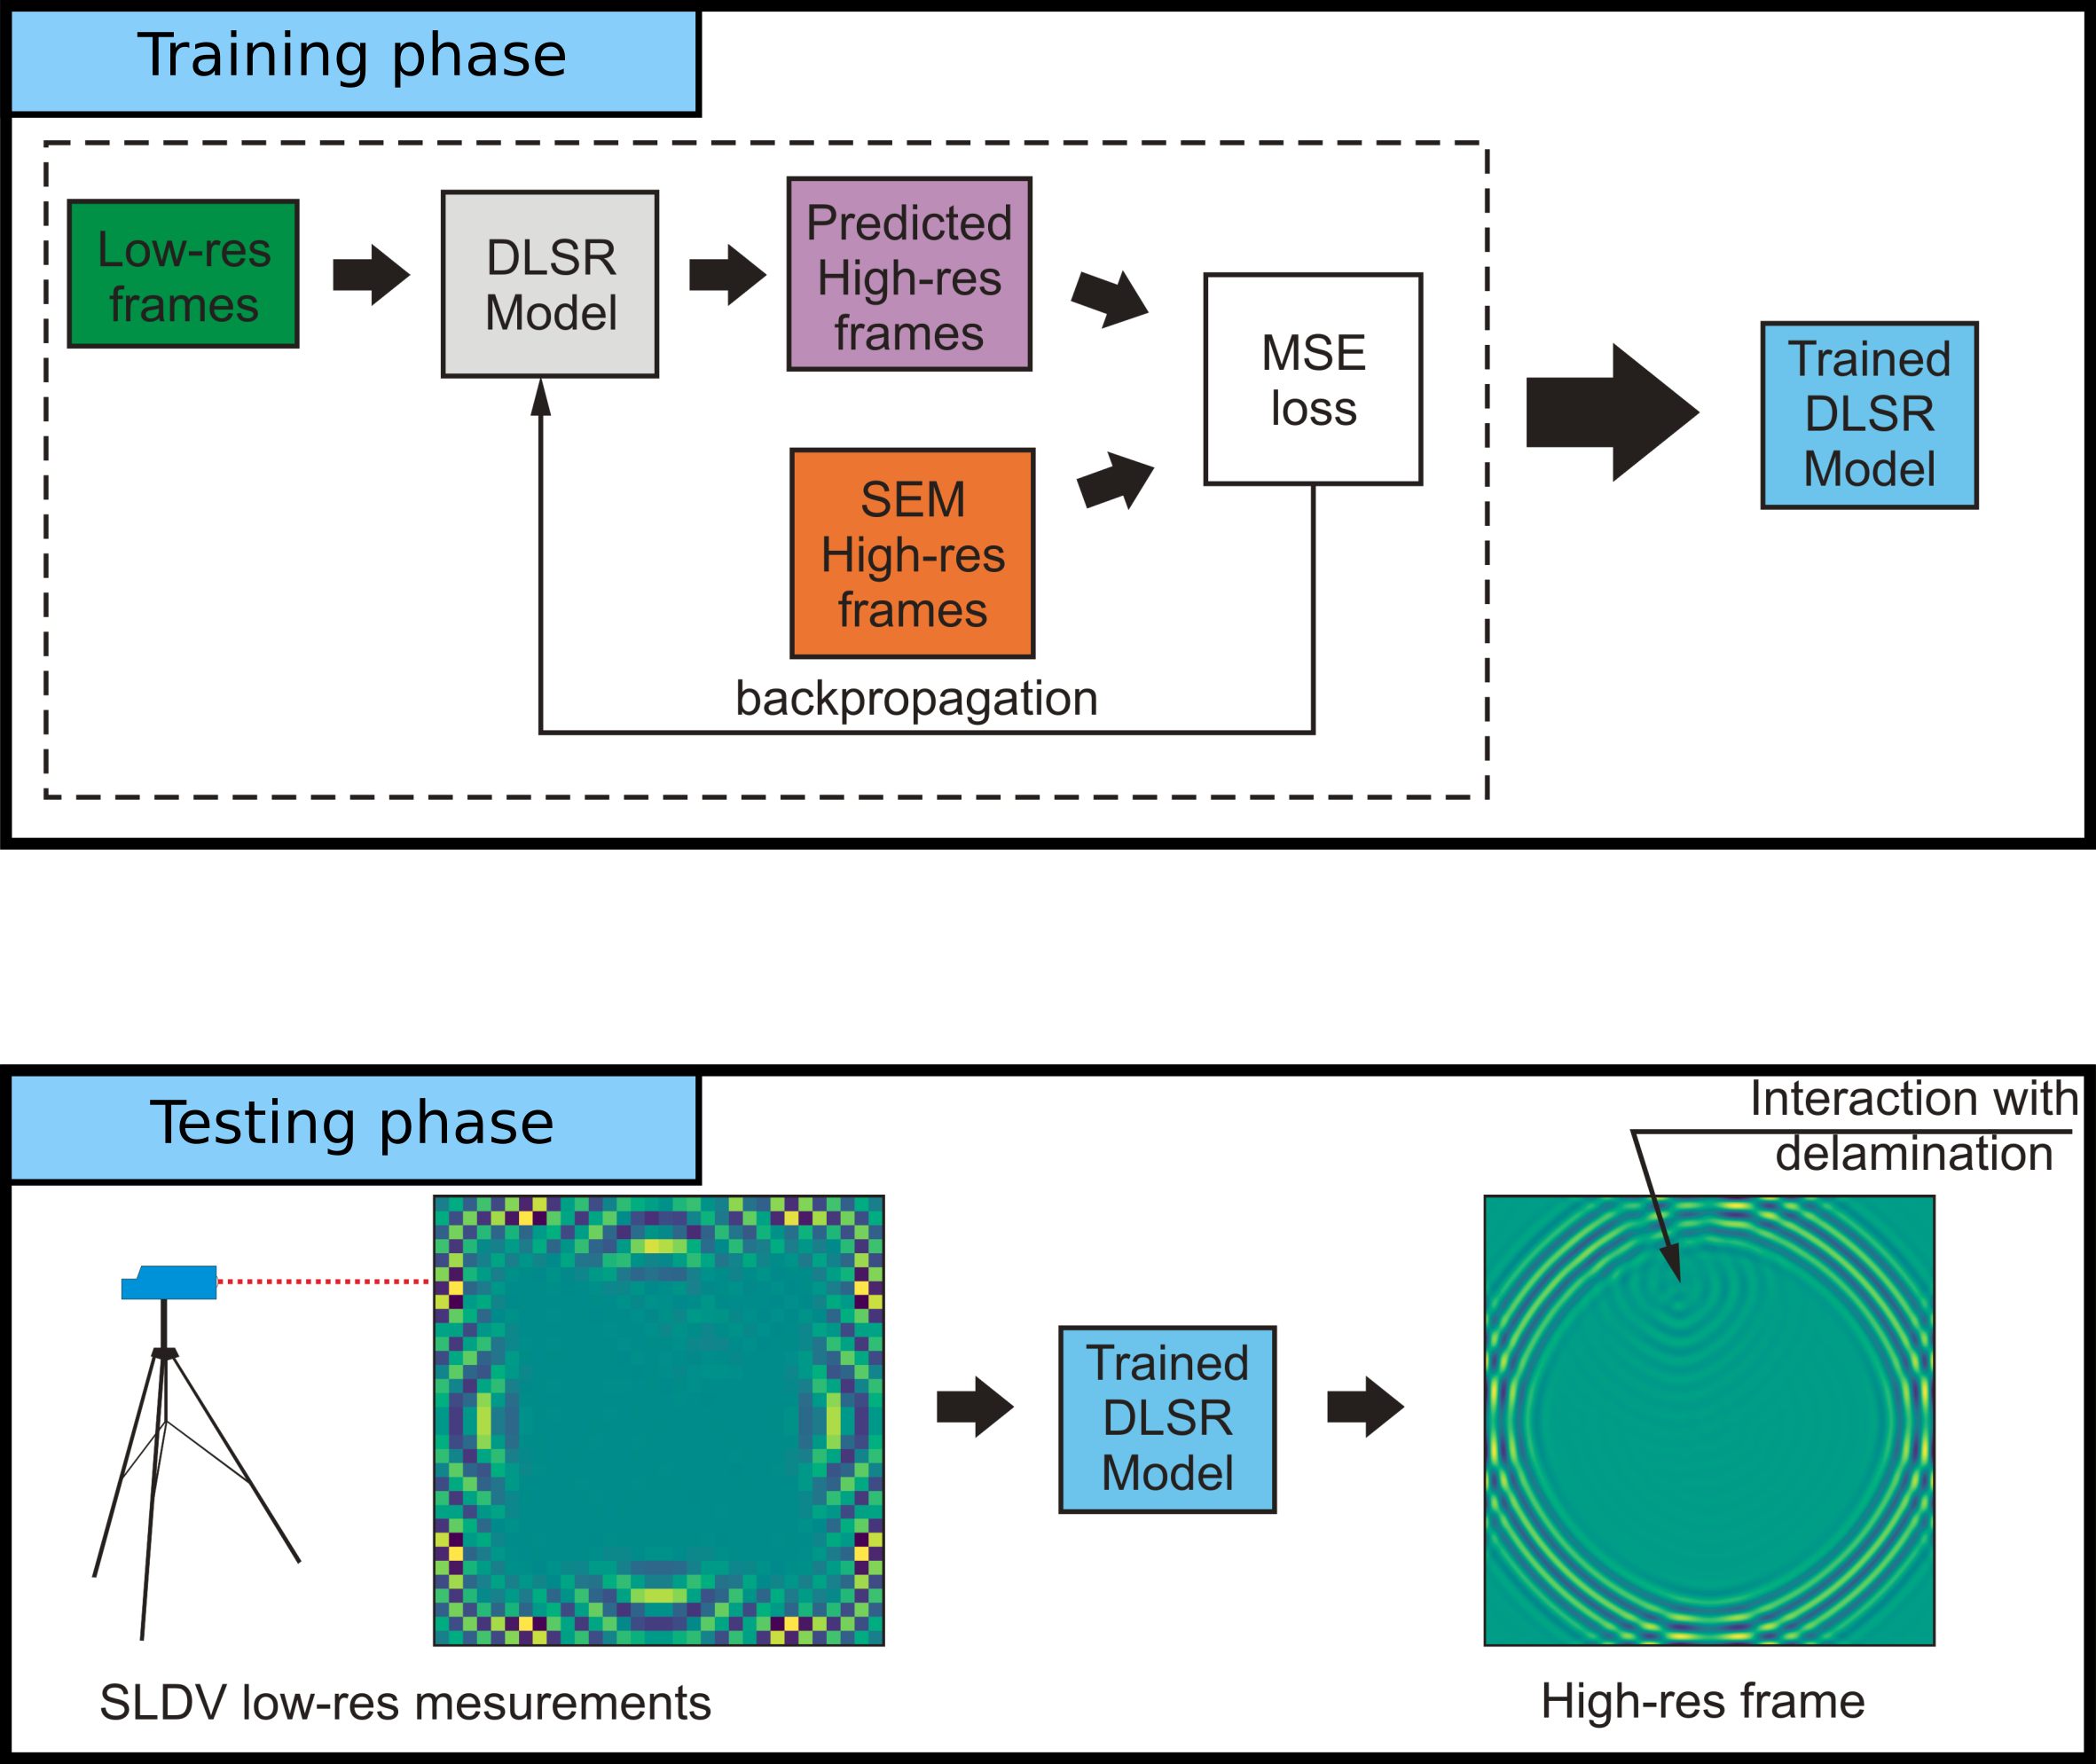
\includegraphics[width=1\textwidth]{superresolution_flowchart.png}
			\end{figure}
		\end{column}
	\end{columns}		
\end{frame}
%%%%%%%%%%%%%%%%%%%%%%%%%%%%%%%%%%%%%%%%%%%%%%%%%%%%%%%%%%%%%%%%%%%%
\note{
	As mentioned earlier, the scanning laser Doppler vibrometer is a well-known non-contact tool for the acquisition of the full wavefield of propagating guided waves.
	However, the process of acquiring the full wavefield of guided waves is time-consuming. 
	One possible solution to tackle this problem is to acquire the Lamb waves at low-resolution grid points, and then the full wavefield can be reconstructed at high resolution.
	Furthermore, I have compared my developed model of deep learning for super-resolution with the compressive sensing technique, which states that any signal can be reconstructed from a linear combination of random measurements.
	To acquire the low-resolution measurements, I have used two types of masks, as shown in the figure: random and jitter.
	The low-resolution measurements are far fewer than required by the Nyquist-Shannon sampling theory.
}

%%%%%%%%%%%%%%%%%%%%%%%%%%%%%%%%%%%%%%%%%%%%%%%%%%%%%%%%%%%%%%%%%%%%
\setcounter{subfigure}{0}
\begin{frame}{Evaluation metrics for DLSR model}
	For evaluating the reconstructed HR full wavefield:
	\begin{itemize}
		\item Peak signal-to-noise ratio (PSNR):
		\begin{equation*}
			PSNR=20\log_{10}\left(\frac{R}{\sqrt{MSE}}\right)
			\label{PSNR_}
		\end{equation*}			
		\item Pearson correlation coefficient (also known as Pearson's r):
		\begin{equation*}
			r_{xy} = \frac{\sum_{i=1}^{n}(x_i - \bar{x})(y_i-\bar{y})}{\sqrt{\sum_{i=1}^{n}(x_i - \bar{x})^2}\sqrt{\sum_{i=1}^{n}(y_i - \bar{y})^2}}
			\label{Pearson_}
		\end{equation*}
	\end{itemize}
\end{frame}
%%%%%%%%%%%%%%%%%%%%%%%%%%%%%%%%%%%%%%%%%%%%%%%%%%%%%%%%%%%%%%%%%%%%
\note
{
	To evaluate the developed model, I used two metrics to measure the quality of the reconstructed high-resolution full wavefield frames:
	\begin{itemize}
		\item The first one is the peak signal-to-noise ratio (PSNR), which refers to the maximum possible power of a signal and the power of the distorting noise that affects the quality of its representation.
		%			This equation depicts the mathematical representation of PSNR, where R is the maximum fluctuation value in the input image, and MSE is the mean squared error between the actual and predicted output.
		%			
		\item The second metric is the Pearson correlation coefficient (Pearson CC), which measures the linear relationship between two
		variable sets \(X\) (represents the ground truth values) and \(Y\) (represents the predicted values) as shown in the below equation.
		
		%			Where \(n\) is the number of sample points,\(x_i, y_i\) are the individual value points representing the ground truth and predicted values, respectively, and \(\bar{x}\) and \(\bar{y}\) are the mean values of the sample and the prediction.
	\end{itemize}
}
%%%%%%%%%%%%%%%%%%%%%%%%%%%%%%%%%%%%%%%%%%%%%%%%%%%%%%%%%%%%%%%%%%%%
\setcounter{subfigure}{0}
\begin{frame}{Numerical test cases}
	\begin{columns}[T]				
		\begin{column}[c]{0.5\textwidth}				
			\begin{figure}
				\centering
				%%%%%%%%%%%%%%%%%%%%%%%%%%%%%%%%%%%%%%%%%%%%%%%%%%%%
				%					\only<1>{
					%						\begin{alertblock}{First test case}
						%							\begin{figure}
							%								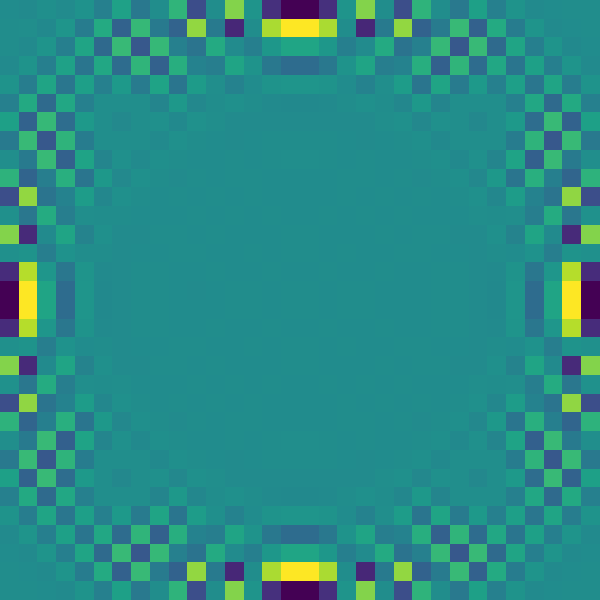
\includegraphics[height=.35\textheight]{LR_456_frame_159_input.png}
							%								\caption{LR input, $f_n=159$}
							%							\end{figure}							
						%							%%%%%%%%%%%%%%%%%%%%%%%%%%%%%%%%%%%%%%%%%%%%
						%							\begin{table}[!h]
							%								\centering 
							%								\footnotesize
							%								\begin{tabular}{cccc}
								%									\toprule
								%									\multicolumn{2}{c}{plate} & \multicolumn{2}{c}{delamination} \\
								%									\cmidrule(lr){1-2} \cmidrule(lr){3-4}
								%									PSNR & PEARSON CC & PSNR & PEARSON CC \\ 
								%									\midrule
								%									42.95 & 0.999 & 33.02 & 0.993 \\					
								%									\bottomrule
								%								\end{tabular}
							%							\end{table}
						%						\end{alertblock}}
				%%%%%%%%%%%%%%%%%%%%%%%%%%%%%%%%%%%%%%%%%%%%%%%%
				\only<1>{
					\begin{alertblock}{First test case}
						\begin{figure}
							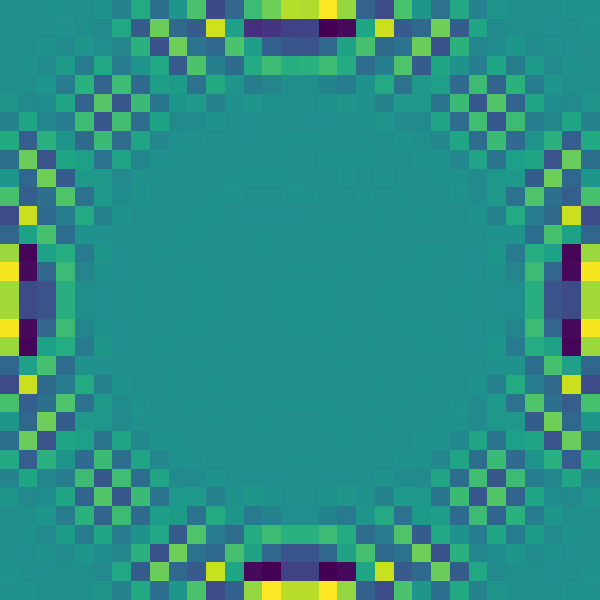
\includegraphics[height=.35\textheight]{LR_438_frame_154_input.png}
							\caption{LR input, $f_n=154$}
						\end{figure}							
						%%%%%%%%%%%%%%%%%%%%%%%%%%%%%%%%%%%%%%%%%%%%
						\begin{table}[!h]
							\centering 
							\footnotesize
							\begin{tabular}{cccc}
								\toprule
								\multicolumn{2}{c}{plate} & \multicolumn{2}{c}{delamination} \\
								\cmidrule(lr){1-2} \cmidrule(lr){3-4}
								PSNR & PEARSON CC & PSNR & PEARSON CC \\ 
								\midrule
								47.00 & 0.998 & 38.52 & 0.995 \\					
								\bottomrule
							\end{tabular}
							\label{tab:num_DLSR_results_2_}
						\end{table}	
						%%%%%%%%%%%%%%%%%%%%%%%%%%%%%%%%%%%%%%%%%%%%
				\end{alertblock}}
				%%%%%%%%%%%%%%%%%%%%%%%%%%%%%%%%%%%%%%%%%%%%%%%%%%%%
				\only<2>{
					\begin{alertblock}{Second test case}
						\begin{figure}
							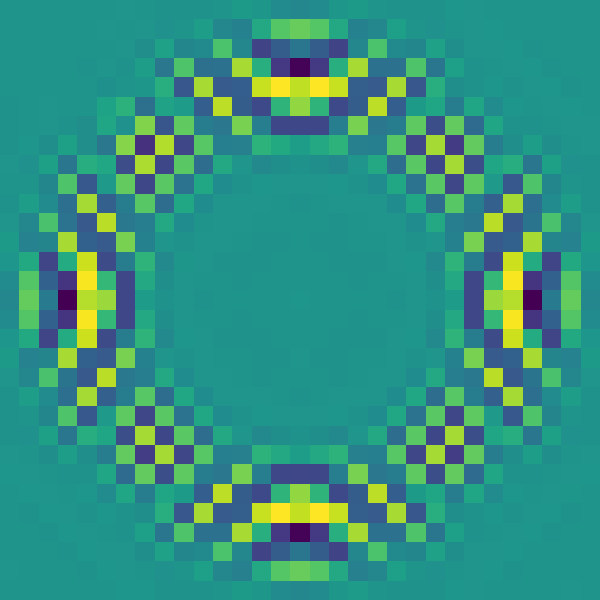
\includegraphics[height=.35\textheight]{LR_397_frame_127_input.png}
							\caption{LR input, $f_n=127$}
						\end{figure}						
						%%%%%%%%%%%%%%%%%%%%%%%%%%%%%%%%%%%%%%%%%%%%
						\begin{table}[!h]
							\centering 
							\footnotesize	
							\begin{tabular}{cccc}
								\toprule
								\multicolumn{2}{c}{plate} & \multicolumn{2}{c}{delamination} \\
								\cmidrule(lr){1-2} \cmidrule(lr){3-4}
								PSNR & PEARSON CC & PSNR & PEARSON CC \\ 
								\midrule
								48.60 & 0.998 & 46.67 & 0.998 \\					
								\bottomrule
							\end{tabular}
						\end{table}
						%%%%%%%%%%%%%%%%%%%%%%%%%%%%%%%%%%%%%%%%%%%%%%%%
				\end{alertblock}}
				%%%%%%%%%%%%%%%%%%%%%%%%%%%%%%%%%%%%%%%%%%%%%%%%%%%%
			\end{figure}
		\end{column}
		%%%%%%%%%%%%%%%%%%%%%%%%%%%%%%%%%%%%%%%%%%%%%%%%%%%%%%%%%%%%
		\begin{column}[c]{0.5\textwidth}
			%				\only<1>{	
				%					\setcounter{subfigure}{0}
				%					\begin{figure}
					%						\subfloat[listentry][HR ref]{
\includegraphics[height=.35\textheight]{output_456_frame_159_full_frame_GT.png}}\quad
					%						\subfloat[listentry][DLSR]{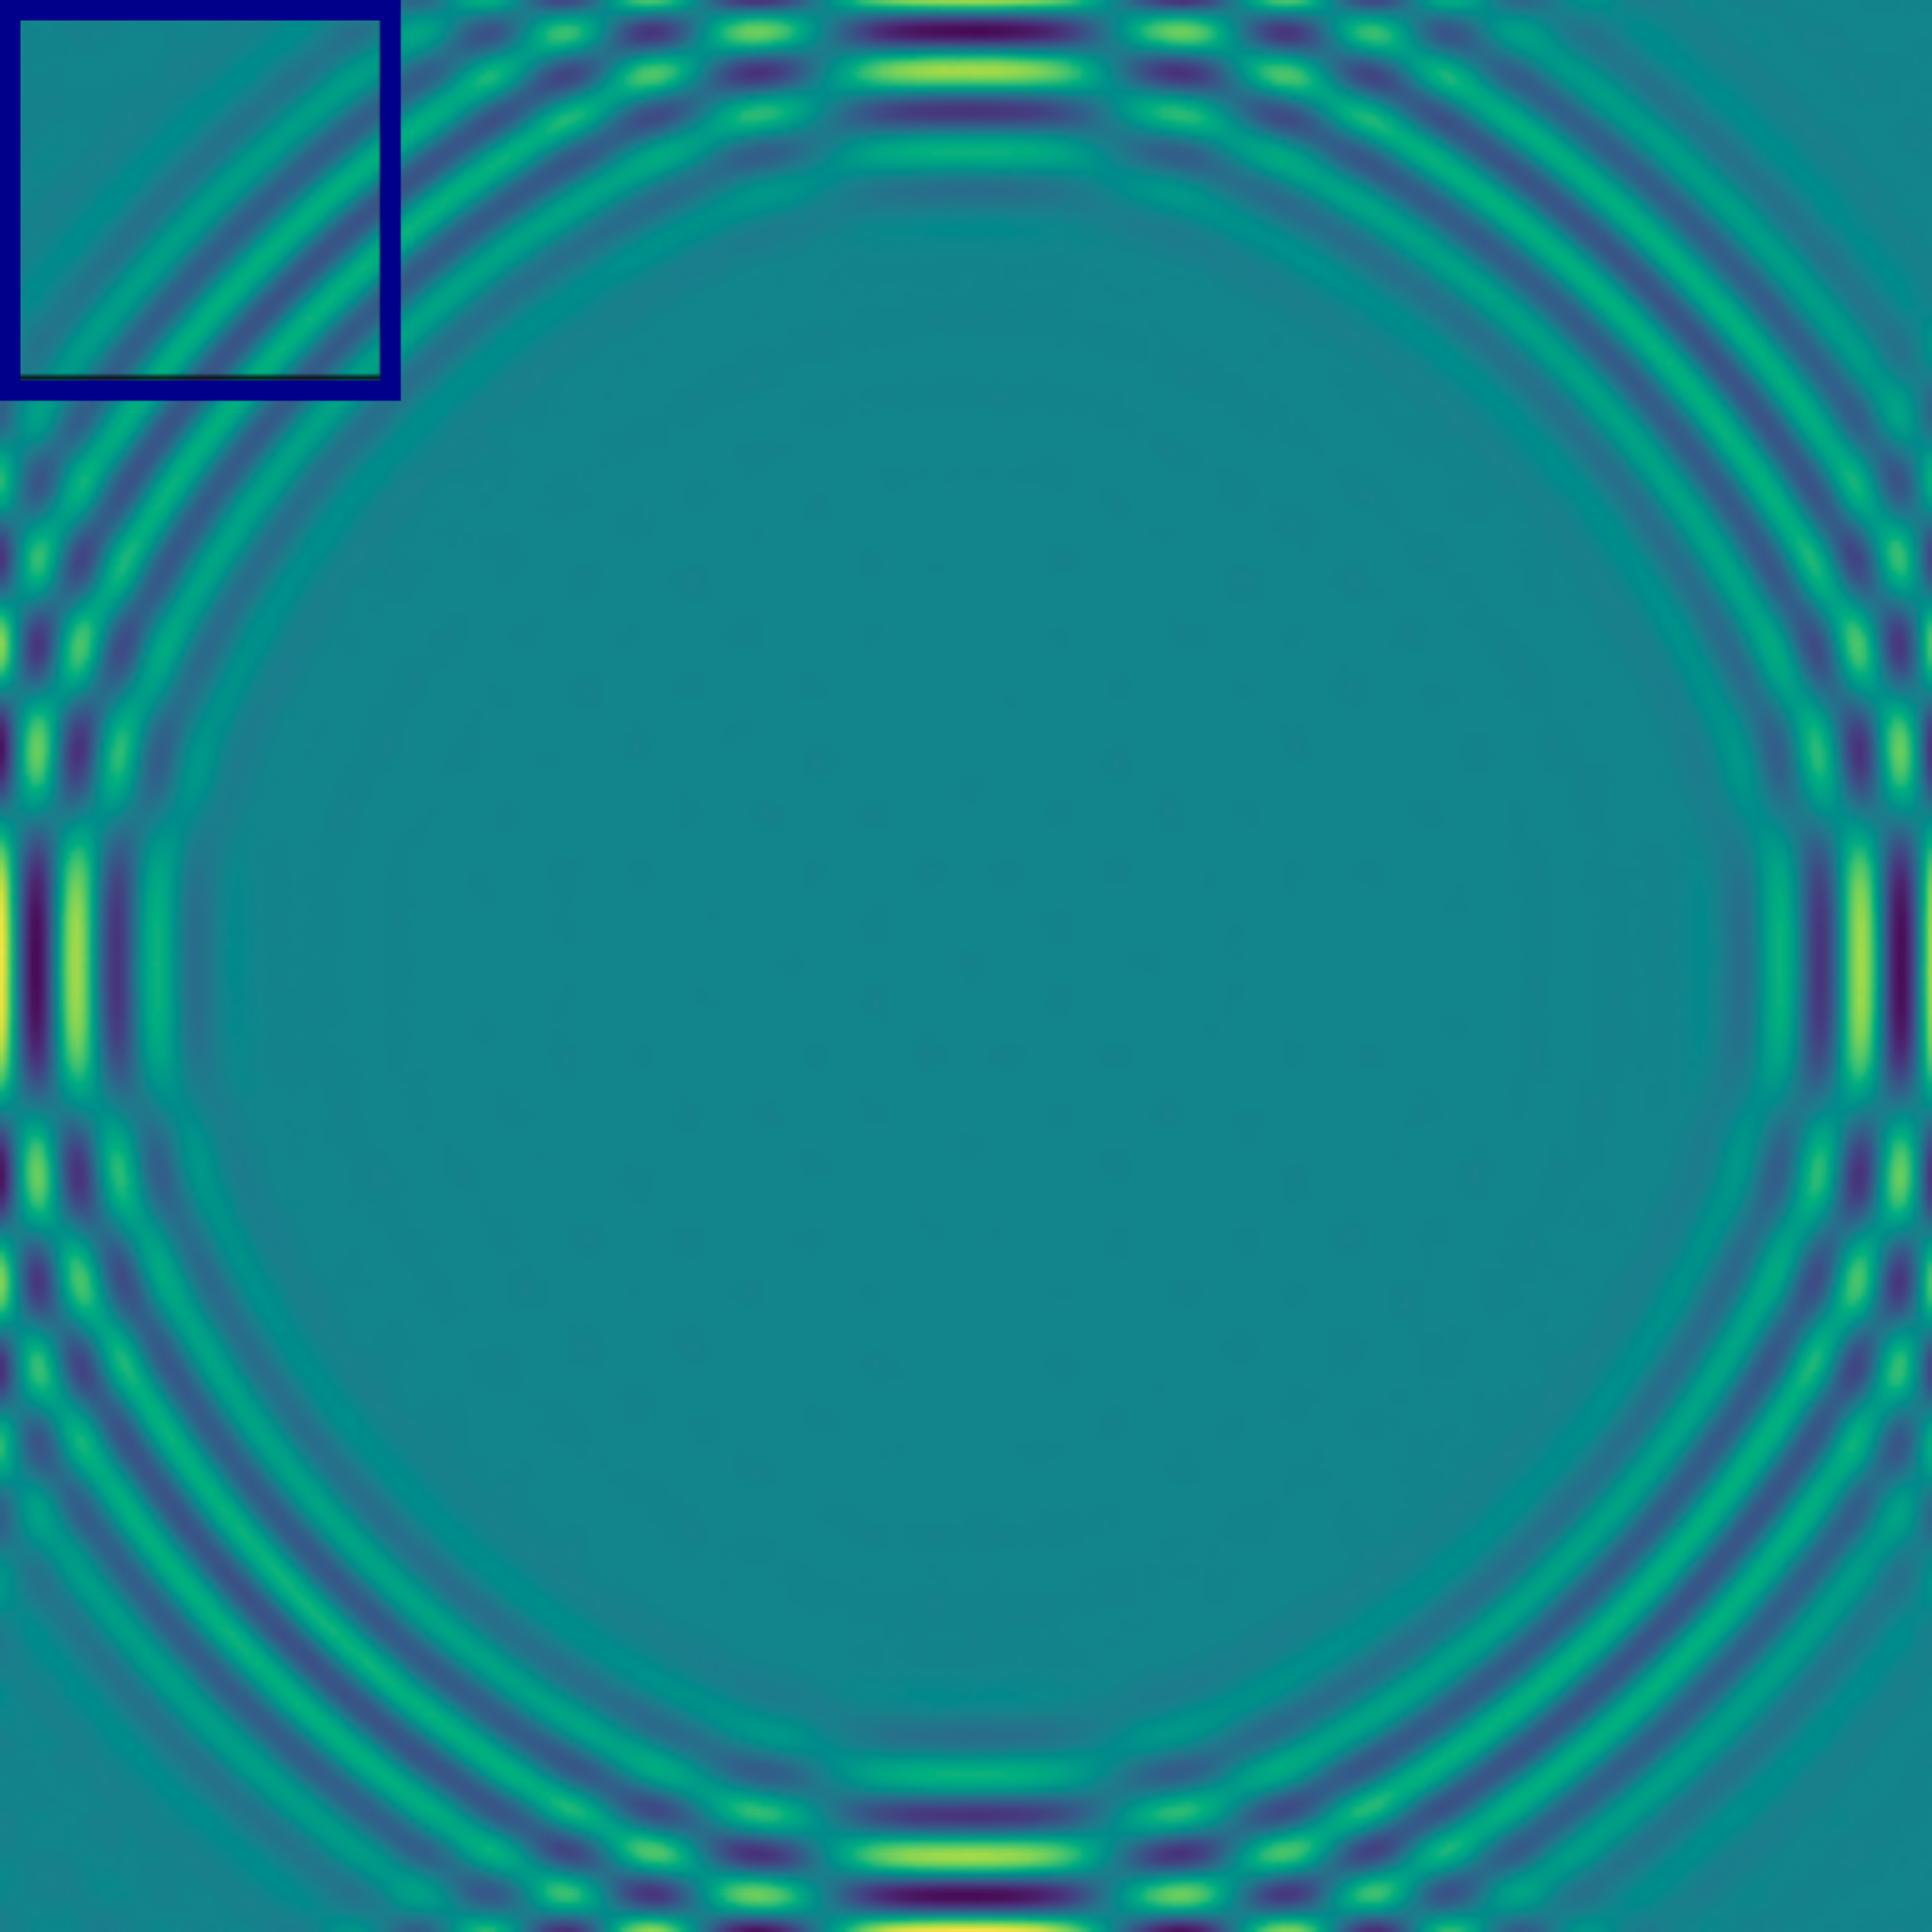
\includegraphics[height=.35\textheight]{output_456_frame_159_full_frame_pred.png}}
					%						\\
					%						\subfloat[listentry][Ref]{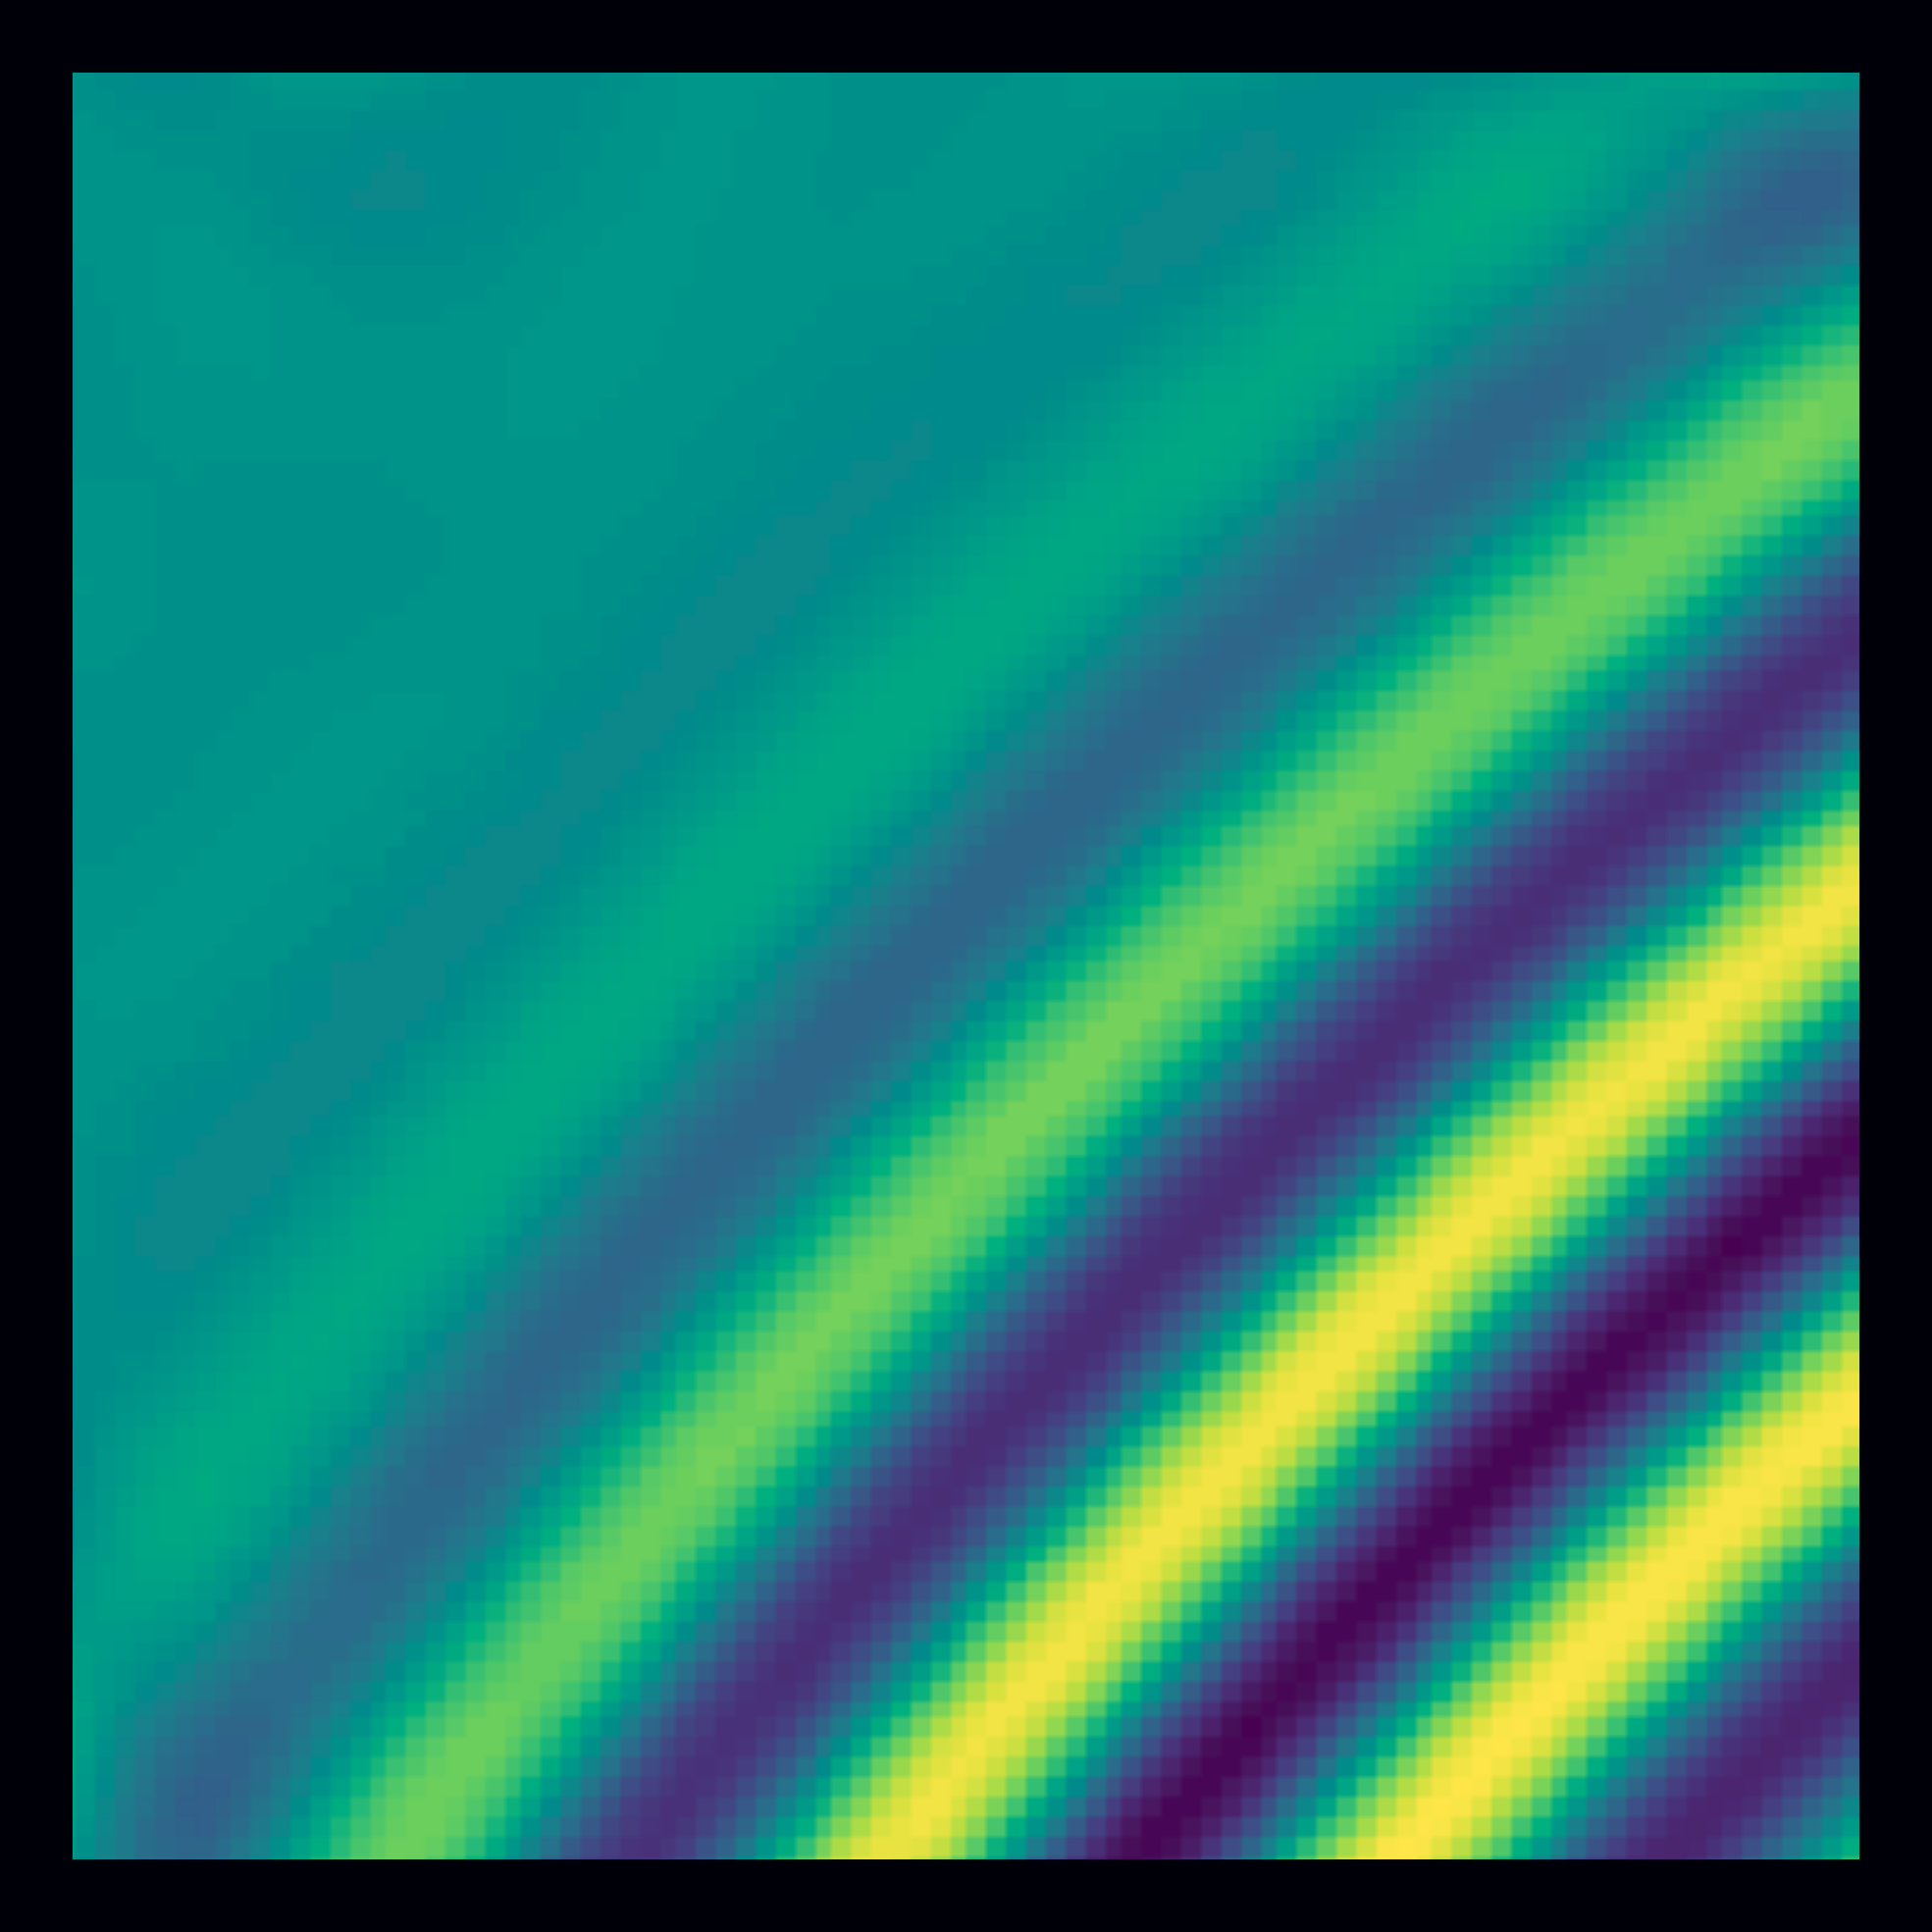
\includegraphics[height=.35\textheight]{output_456_frame_159_delamination_GT.png}}\quad
					%						\subfloat[listentry][DLSR]{\includegraphics[height=.35\textheight]{output_456_frame_159_delamination_pred.png}}
					%					\end{figure}}			
			\only<1>{
				\setcounter{subfigure}{0}					
				%%%%%%%%%%%%%%%%%%%%%%%%%%%%%%%%%%%%%%%%%%%%%%%%%%%%
				\begin{figure}
					\subfloat[listentry][HR ref]{\includegraphics[height=.35\textheight]{output_438_frame_154_full_frame_GT.png}}\quad
					\subfloat[listentry][DLSR]{\includegraphics[height=.35\textheight]{output_438_frame_154_full_frame_pred.png}}
					\\
					\subfloat[listentry][Ref]{\includegraphics[height=.35\textheight]{output_438_frame_154_delamination_GT.png}}\quad	
					\subfloat[listentry][DLSR]{\includegraphics[height=.35\textheight]{output_438_frame_154_delamination_pred.png}}
			\end{figure}}
			\only<2>{	
				\setcounter{subfigure}{0}
				\begin{figure}
					\centering
					\subfloat[listentry][HR ref]{\includegraphics[height=.35\textheight]{output_397_frame_127_full_frame_GT.png}}\quad
					\subfloat[listentry][DLSR]{\includegraphics[height=.35\textheight]{output_397_frame_127_full_frame_pred.png}}
					\\
					\subfloat[listentry][Ref]{\includegraphics[height=.35\textheight]{output_397_frame_127_delamination_GT.png}}\quad
					\subfloat[listentry][DLSR]{\includegraphics[height=.35\textheight]{output_397_frame_127_delamination_pred.png}}
			\end{figure}}
		\end{column}
	\end{columns}
\end{frame}
%%%%%%%%%%%%%%%%%%%%%%%%%%%%%%%%%%%%%%%%%%%%%%%%%%%%%%%%%%%%%%%%%%%%
\note
{
	\footnotesize
	In the following, the results of the reconstruction of HR frames for two numerical test cases will be presented.				
	
	In the first test case, the figure shows the low-resolution measurements at frame number 154.		
	Figure a shows the actual HR frame, and figure b shows the predicted SR frame. 
	The PSNR value is 47
	
	Figure c shows the HR sub-frame at the delamination region, figure d shows the SR prediction at the delamination region, and the PSNR is 38.52.
	
	In the second test case, the figure shows the low-resolution measurements at frame number 127.
	Figure a shows the actual HR frame, and figure b shows the predicted SR frame. 
	The PSNR value is 42.95
	
	Figure c shows the HR sub-frame at the delamination region, figure d shows the SR prediction at the delamination region, and the PSNR is 33.02.
	
	
}
%%%%%%%%%%%%%%%%%%%%%%%%%%%%%%%%%%%%%%%%%%%%%%%%%%%%%%%%%%%%%%%%%%%%
\setcounter{subfigure}{0}
\begin{frame}{Experimental test case}		
	\begin{columns}[T]
		%%%%%%%%%%%%%%%%%%%%%%%%%%%%%%%%%%%%%%%%%%%%%%%%%%%%%%%%%%%%
		\begin{column}[t]{0.25\textwidth}				
			\begin{figure}	
				\centering					
				\includegraphics[width=1\textwidth]{frame110_32x32.png}
				%					\caption{LR input \((N_f = 110)\)}
			\end{figure}
			\footnotesize
			LR measurements (Input): \(32\times32=1024\)p. \\
			HR (Output): \(512\times512=262144\)p.
		\end{column}
		%%%%%%%%%%%%%%%%%%%%%%%%%%%%%%%%%%%%%%%%%%%%%%%%%%%%%%%%%%%%
		\begin{column}[t]{.25\textwidth}
			\begin{block}{HR label}
				\begin{figure}
					\centering
					\subfloat{\includegraphics[width=0.75\textwidth]{figure10a.png}}
					\vfill
					\subfloat{\includegraphics[width=0.75\textwidth]{figure11a.png}}
				\end{figure}
			\end{block}
		\end{column}
		%%%%%%%%%%%%%%%%%%%%%%%%%%%%%%%%%%%%%%%%%%%%%%%%%%%%%%%%%%%%
		\begin{column}[t]{.25\textwidth}
			\begin{block}{CS: 1024p}
				\begin{figure}
					\centering
					\subfloat{\includegraphics[width=0.75\textwidth]{figure10b.png}}
					\vfill						
					\subfloat{\includegraphics[width=0.75\textwidth]{figure11b.png}}
				\end{figure}
			\end{block}				
		\end{column}
		%%%%%%%%%%%%%%%%%%%%%%%%%%%%%%%%%%%%%%%%%%%%%%%%%%%%%%%%%%%%
		\begin{column}[t]{.25\textwidth}
			\begin{alertblock}{DLSR}
				\begin{figure}
					\centering
					\subfloat{\includegraphics[width=0.75\textwidth]{figure10e.png}}
					\vfill			
					\subfloat{\includegraphics[width=0.75\textwidth]{figure11e.png}}\quad
				\end{figure}
			\end{alertblock}				
			%%%%%%%%%%%%%%%%%%%%%%%%%%%%%%%%%%%%%%%%%%%%%%%%%%%%%%%%%%%%
		\end{column}				
	\end{columns}
\end{frame}
%%%%%%%%%%%%%%%%%%%%%%%%%%%%%%%%%%%%%%%%%%%%%%%%%%%%%%%%%%%%%%%%%%%%
\note{
	\footnotesize
	In this slide, I present an experimental test case,
	
	The figure on the left represents an experimentally acquired full wavefield in it low resolution.	
	
	This Figure shows the actual HR reference frame for the whole plate and at the delamination area
	
	The figure in the middle represents the outputs of applying the compressive sensing technique in which it shows a poor quality of reconstruction. 
	
	
	The figure on the right presents the reconstructed HR frame with the DLSR model for the whole plate and at the delamination area as you can see the quality of reconstruction is very noticeable. 
}
%%%%%%%%%%%%%%%%%%%%%%%%%%%%%%%%%%%%%%%%%%%%%%%%%%%%%%%%%%%%%%%%%%%%
\begin{frame}{Analysis of experimental case}
	\begin{table}[!ht]
		\renewcommand{\arraystretch}{1.3}
		\centering \footnotesize
		\caption{Quality metrics for tested methods.}	
		\begin{tabular}{lrrrcrc} 
			\toprule[1.5pt]
			& & & \multicolumn{2}{c}{plate} & \multicolumn{2}{c}{delamination} \\
			\cmidrule(lr){4-5} \cmidrule(lr){6-7}
			Method & $N_p$ & CR [\%] & PSNR & PEARSON CC& PSNR & PEARSON CC \\
			\midrule
			\csvreader
			[table head=\toprule,
			late after line=\\ 
			]{table_metrics.csv}{
				1=\one, 2=\two, 3=\three, 4=\four, 5=\five, 6=\six, 7=\seven
			}%
			{\one & \two & \three & \four & \five & \six & \seven }%	
			\bottomrule[1.5pt]
		\end{tabular}	
		\label{tab:csv_results_}
	\end{table}
\end{frame}
%%%%%%%%%%%%%%%%%%%%%%%%%%%%%%%%%%%%%%%%%%%%%%%%%%%%%%%%%%%%%%%%%%%%
\note{
	The following table presents a detailed comparison of the quality metrics for CS methods with applied jitter and random masks and the DLSR model.
	As shown in the table the DLSR model achieved the highest PSNR and Pearson CC values.		
}
%%%%%%%%%%%%%%%%%%%%%%%%%%%%%%%%%%%%%%%%%%%%%%%%%%%%%%%%%%%%%%%%
\section{Conclusions}
%%%%%%%%%%%%%%%%%%%%%%%%%%%%%%%%%%%%%%%%%%%%%%%%%%%%%%%%%%%%%%%%
\begin{frame}{Conclusions}		
	\begin{footnotesize}
		\begin{justify}
			\settowidth{\leftmargini}{\usebeamertemplate{itemize item}}
			\addtolength{\leftmargini}{\labelsep}
			\begin{itemize}
				\item{Deep learning models trained on synthetic dataset generalise well and can be applied directly to experimental wavefields.}			
				\item{Deep learning approaches surpass conventional approaches for delamination identification.}	
				\item{Animation-based deep learning models perform better than image-based models but are more complex and require longer time for training.}					
				\item{Deep learning models can be generalised to other types of defects and materials.}
				\item{The DLSR model can recover the HR measurements from LR measurements with good accuracy.}
			\end{itemize}
		\end{justify}									
	\end{footnotesize}			
\end{frame}			
\note{}	
%%%%%%%%%%%%%%%%%%%%%%%%%%%%%%%%%%%%%%%%%%%%%%%%%%%%%%%%%%%%%%%%%%%
\setcounter{subfigure}{0}
%%%%%%%%%%%%%%%%%%%%%%%%%%%%%%%%%%%%%%%%%%%%%%%%%%%%%%%%%%%%%%%%%%%%
{
	\setbeamercolor{palette primary}{fg=blue, bg=white}
	\begin{frame}[standout]
		\centering
		Thank you for your listening!\\ \vspace{12pt}
		Questions?\\ \vspace{12pt}
		\url{abdalraheem.ijjeh@gmail.com}
	\end{frame}
}
\note{}	
%	%%%%%%%%%%%%%%%%%%%%%%%%%%%%%%%%%%%%%%%%%%%%%%%%%
\end{document}